\documentclass[a4paper,12pt,oneside]{book}
\usepackage[cp1250]{inputenc}
\usepackage{czech}
\usepackage{graphicx}
\usepackage{amssymb}
\usepackage{amsmath}
\usepackage{amsthm}
\usepackage{algorithmicx}
\usepackage{subfig}
\usepackage[Algoritmus]{algorithm}
\usepackage{algpseudocode}
\usepackage{float}
\usepackage{listings}
\usepackage{multirow}
\usepackage{color}
\usepackage{booktabs}
\usepackage{rotating}

\newenvironment{CompactItemize}
{
  \begin{itemize}
  \setlength{\itemsep}{-3pt}
  \setlength{\parsep}{0pt}
  \setlength{\topsep}{0pt}
  \setlength{\partopsep}{0pt}
} 
{\end{itemize}}

\newenvironment{CompactList}
{\begin{list}{}{
  \setlength{\leftmargin}{0.5cm}
  \setlength{\itemsep}{0pt}
  \setlength{\parsep}{0pt}
  \setlength{\topsep}{0pt}
  \renewcommand{\makelabel}{}}}
{\end{list}}

\newenvironment{BulletList}
{\begin{itemize}
   \setlength{\itemsep}{0pt}
}
{\end{itemize}}

\newcommand{\code}[1] {\noindent \texttt{#1}\\}

\newcommand{\codeskip}[1] {\hskip 1cm \texttt{#1}\\}

\newcommand{\protocol}[1] {\noindent {\small \texttt{#1}}}

\newcommand{\abstrakt}[1] {\noindent {\textit{#1}}}

\newcommand{\keywords}[1] {\small {#1} \normalsize}




\let\oldmarginpar\marginpar
\renewcommand\marginpar[1]{\-\oldmarginpar[\raggedleft\footnotesize #1]%
{\raggedright\footnotesize \textcolor{red}{#1}}}


\newcommand{\FuncReturn}[1] {\State \textbf{return} {#1}}

\newtheorem{theorem}{V�ta}[section]
\newtheorem{lemma}[theorem]{Lemma}
\newtheorem{proposition}[theorem]{Tvrzen�}
\newtheorem{corollary}[theorem]{D�sledek}

%\newenvironment{proof}[1][D�kaz]{\begin{trivlist}
%\item[\hskip \labelsep {\bfseries #1}]}{\end{trivlist}}

\newenvironment{definition}[1][Definice]{\begin{trivlist}
\item[\hskip \labelsep {\bfseries #1.}]}{\end{trivlist}}

\newenvironment{example}[1][P��klad]{\begin{trivlist}
\item[\hskip \labelsep {\bfseries #1}]}{\end{trivlist}}

\newenvironment{remark}[1][Pozorov�n�]{\begin{trivlist}
\item[\hskip \labelsep {\bfseries #1}]}{\end{trivlist}}

\newcommand{\param}[1] {\emph{#1}}


\begin{document}
\lstset{language=C++}
\input epsf
\pagenumbering{gobble}

\pagestyle{plain}
%\pagestyle{empty}
\begin{center}
Univerzita Karlova v Praze\\Matematicko-fyzik�ln� fakulta\\
\addvspace{40pt}

\textbf{DIPLOMOV� PR�CE}\\

\addvspace{40pt}

\putpicscalenocaption{0.70}{img/logo.eps}

\addvspace{40pt}
 
Jakub Kotrla\\

\addvspace{10pt}

\textbf{Prostorov� mapy pro agenty imituj�c� lidsk� chov�n�}\\

\addvspace{20pt}
Kabinet software a v�uky informatiky\\
Vedouc� diplomov� pr�ce: Mgr. Cyril Brom, Ph.D.\\
Studijn� program: Informatika, softwarov� syst�my\\
\bigskip
2009
\end{center}

\begin{titlepage}

%\large
%\noindent
%\textbf{Pod�kov�n�}\\
%\normalsize
%\noindent
%R�d bych zde pod�koval m�mu vedouc�mu RNDr. Franti�ku Mr�zovi, CSc. za cenn� rady, konzultace a veden�. Tak� m� p��telkyni Hance a rodin� za trp�livost a podporu, kterou projevovali po celou dobu psan� t�to pr�ce. D�kuji.

\begin{figure}[b]
 Prohla�uji, �e jsem svou diplomovou pr�ci napsal samostatn� a v�hradn� s~pou�it�m citovan�ch pramen�. Souhlas�m se zap�j�ov�n�m pr�ce.\\[2em]
\begin{tabular*}{1.0\textwidth}[b]{@{\extracolsep{\fill}}lr}
V Praze, \today\\
\end{tabular*}
\end{figure}
\end{titlepage}

\pagebreak


\tableofcontents

%\pagestyle{empty}

\noindent \textbf{N�zev pr�ce:}  Prostorov� mapy pro agenty imituj�c� lidsk� chov�n�\\
\noindent \textbf{Autor:} Jakub Kotrla\\
\noindent \textbf{Katedra (�stav):} Kabinet software a v�uky informatiky\\
\noindent \textbf{Vedouc� diplomov� pr�ce:} Mgr. Cyril Brom, Ph.D.\\
\noindent \textbf{e-mail vedouc�ho:} brom@ksvi.mff.cuni.cz\\
\noindent \textbf{Abstrakt:} \abstrakt{C�lem t�to pr�ce je....}\\
\noindent \textbf{Kl��ov� slova:} prostorov� mapa, \\
\newline
\noindent \textbf{Title:} Spatial maps for virtual agents imitating human behaviour\\
\noindent \textbf{Author:} Jakub Kotrla\\
\noindent \textbf{Department:} Department of Software and Computer Science Education\\
\noindent \textbf{Supervisor:} Mgr. Cyril Brom, Ph.D.\\
\noindent \textbf{Supervisor's e-mail address:} brom@ksvi.mff.cuni.cz\\
\noindent \textbf{Abstract:} \abstrakt{The goal of this thesis is ....}\\
\noindent \textbf{Keywords:} spatial map\\
\pagenumbering{arabic}
\setcounter{page}{1}

\chapter{�vod}

Ka�d� �iv� tvor m� pam�, tedy schopnost ulo�it si informaci a pozd�ji si ji vybavit a pou��t.
Pam� je d�le�it�m p�edpokladem pro inteligentn� chov�n� jedince, bez n� nebude schopen se u�it nov� informace a dovednosti.
\\

Lidskou pam� je mo�n� d�lit dle mnoha krit�ri�.
Nap�. dle trvalosti uchov�van�ch z�znam� na kr�tkodobou a dlouhodobou.
Kr�tkodob� pam� um� uchovat jen velmi omezen� mno�stv� informac� na kr�tkou dobu, kter� p�edstavuje ��dov� sekundy a� minuty.
Naopak dlouhodob� pam� je schopn� uchovat informaci po n�kolik dn� a� po cel� �ivot jedince a jej� kapacita se zd� neomezen�.
D�le je pam� mo�n� d�lit dle povahy informac�, kter� ukl�d�. T�mto zp�sob�m se pam� obvykle d�l� na procedur�ln�, s�mantickou a episodickou.
Procedur�ln� pam� ukl�d� zp�soby pou�it� p�edm�t� a pohyby, kter� �lov�k prov�d� bez pln�ho soust�ed�n�, nap�. j�zda na kole.
S�mantick� pam� obsahuje objektivn� fakta o okoln�m sv�t�, nap�. kolik m� t�den dn� nebo jakou barvu m� zebra.
Episodick� pam� je pam�t� na osobn� ud�losti, z�itky, subjektivn� informace,
kter� se v�� k vlastn� osob�, nap�. co d�lal �lov�k v�era ve�er �i kdy naposledy jedl.
\\

%litTulving

Sou��st� pam�ti je i prostorov� mapa sv�ta, kter� b�v� ch�p�na jako ��st episodick� pam�ti.
Prostorov� mapa n�m umo��uje plnit jednoduch� ka�dodenn� �koly jako je navigace v prostoru, ur�en� polohy p�edm�t�,
ale i slo�it�j�� �lohy, nap�. popisov�n� cesty jin�mu �lov�ku, pl�nov�n� staveb �i st�hov�n� apod.
\\


V sedmdes�t�ch letech dvac�t�ho stolet� popsali psychologov� u potkan� tzv. \emph{place cells} \cite{litPlaceCells1,litPlaceCells2}.
Place cells jsou neurony hippocampu, kter� vykazuj� m�stn� specifickou aktivitu � jsou aktivn�, je-li potkan v ur�it�m m�st� v prostoru.
Reaguj� i na dal�� neprostorov� informace a objekty, tak� na zm�ny prost�ed�.
\\

V n�sleduj�c�ch letech byly u potkan� objeveny a pops�ny dal�� typy neuron�, jejich� aktivita souvis� s prostorem a orientac�.
Neurony, kter� jsou aktivn� dle sm�ru nato�en� hlavy potkana �i kter� jsou aktivn� v bl�zkosti hranic prostoru \cite{litHDcells1,litHDcells2,litBorderCells}.
V�zkum ukazuje, �e neurony s podobn�mi vlasnostmi jako jsou place cells, maj� i lid� \cite{litPlaceCellsHuman,litPlaceCellsHuman2}.
\\

%Vn�m�n�, pozornost, r�zn� reprezentace - alocentrick� a egocentrick�

C�lem pr�ce je vytvo�it model prostorov� mapy, kter� umo�n� imitovat lidsk� chov�n�.
Mezi to pat�� p�edev��m nep�esnost a postupn� u�en� se prostoru, rozlo�en� p�edm�t� a schopnost p�izp�sobit se zm�n�m.
Dal�� typickou vlasnost� lidsk� pam�ti, kter� se t�k� i prostorov� mapy, je zapom�n�n�.
Po ur�it� dob� si �lov�k nen� schopen vzpomenout, kde p�esn� na poli�ce m� v kuchyni s�l, pozd�ji si nebude jist�, ani na kter� poli�ce s�l je. 
V pr�b�hu �asu by model m�l zapom�nat, nejd��ve detaily a pozd�ji i obecn�j�� informace o prostoru a um�st�n� p�edm�t�.
�lov�k vn�m� p�edm�ty na jednom m�st� jako skupinu p�edm�t�, prostorov� informace si shlukuje a vytv��� hiearchii.
\\

Model prostorov� mapy bude vych�zet z v�sledk� v�zkumu place cells.
Navrhneme jej a budeme zkoumat jeho chov�n� v r�zn�ch p��padech, vliv parametr�  apod.
Model budeme posuzovat subjektivn�.
D�le zkus�me naj�t objektivn� metriky, kter� by n�m mohli pomoci v hodncen� modelu, nap�. podobnost mapy s virtu�ln�m sv�tem.
\\



Pr�ce je rozd�lena do osmi kapitol.
Po t�to �vodn� kapitole n�sleduje druh� kapitola, kter� podrobn� rozeb�r� �e�en� probl�m, vyjmenov�v� po�adavky a omezen�.
Ve t�et� kapitole jsou shrnuty n�kter� dosavadn� pr�ce, kter� by bylo mo�n� pou��t �i alespo� z nich vyj�t.
�tvrt� kapitola popisuje abstrakci sv�ta a architekturu agenta pou�it�ho pro tvorbu a zkoum�n� modelu,
p�t� kapitola p�edstavuje v�sledn� model v�etn� slep�ch v�tv� a rozhodnut� a z�kladn�ch test�.
\\

�e�t� kapitola je v�nov�na test�m modelu na r�zn�ch datech, s r�zn�m nastaven�m parametr� a men��ch �prav modelu.
Na v�sledc�ch ukazuje vliv zm�n r�zn�ch parametr� a vzorc�.
V sedm� kapitole jsou pops�na dal�� mo�n� roz���en� modelu a nazna�eny dal�� mo�n� sm�ry jeho v�voje a v�zkumu,
v osm� kapitole jsou shrnuty v�sledky pr�ce.
Na p�ilo�en�m CD je prototypov� aplikace pou�it� pro testov�n� modelu a v�sledky v�ech proveden�ch test�.
\\

\chapter{Rozbor probl�mu} \label{chapter-rozbor}

C�lem pr�ce je vytvo�it model prostorov� mapy, kter� bude agentovi umo��ovat imitovat lidsk� chov�n�.
V t�to kapitole pop�eme po�adavky na model, jeho vstupy a v�stupy.
\\

Agent m� na za��tku �plnou informaci o geometrii a topologii sv�ta. V pr�b�hu simulace se agent pohybuje sv�tem a vn�m� sv� okol�.
V ka�d�m okam�iku v�, kde p�esn� se nal�z�, kter�m sm�rem se d�v�, jak� p�edm�ty vid� a kde jsou tyto p�edm�ty ve virtu�ln�m sv�t� um�st�ny.
Agent si tedy nemus� vytv��et mapu, ani �e�it anal�zu obrazov�ch dat �i podobn� �lohy z robotiky. Dost�v� p�esn� geometrick� data - nap�:

\emph{Stoj�m na sou�adnic�ch XY, d�v�m se sm�rem na severoz�pad. Vid�m dva p�edm�ty: kv�tinu a tal��. Kv�tina je na sou�adnic�ch XZ, tal�� na YZ.}
\\

\begin{definition}[Uzel]
Prostorov� mapa bude obsahovat \emph{uzly}. Uzel je bod v prostoru, kter� reprezentuje resp. pokr�v� jeho ��st, sv� okol�. Imituje tak chov�n� place cells.
Model mus� um�t na za��tku simulace tyto uzly rozm�stit do virtu�ln�ho sv�ta.
V pr�b�hu simulace mus� jejich rozm�st�n� postupn� m�nit, tak aby jejich hustota byla v�t�� v m�stech, kde agent vid�l v�ce p�edm�t�, a men�� v m�stech,
kde agent vid�l m�n� p�edm�t�. Nejmen�� hustota by m�la b�t v m�stech, kde agent nevid�l ��dn� p�edm�ty �i kter� v�bec nenav�t�vil.
I v takov�chto m�stech ale mus� b�t uzly mapy.
\end{definition}

Model mus� umo�nit ukl�dat k uzl�m informace o poloze p�edm�t�. Tyto informace si m��e agent pozd�ji vy��dat.
P�esnost t�chto informac� by m�la v �ase r�st, pokud je agent opakovan� dost�v�. Naopak pokud agent informaci o poloze p�edm�t� del�� dobu nedostane,
informace by se m�la st�t nep�esnou a postupn� vymizet, a� do t� m�ry, �e agent bude schopen ��ci pouze to, �e p�edm�t vid�l, nebude v�ak schopen ur�it kde.
\\

Po�et uzl� prostorov� mapy by se m�l p�izp�sobit velikosti sv�ta a po�tu p�edm�t� v n�m.
Sou��st� modelu tedy mus� b�t mechanismus koriguj�c� po�et uzl� mapy v �ase, v z�vislosti na po�tu p�edm�t�, kter� agent vid�, resp. �etnosti vjem� p�edm�t�.
\\

Model by m�l b�t hiearchick� �i alespo� umo�nit vytvo�en� hiearchie.
V�echny uzly mapy by nem�ly b�t rovnocenn�, v pr�b�hu simulace by m�ly vznikat dal�� uzly vy��� �rovn�, kter� budou pokr�vat v�t�� oblast.
Tyto uzly by m�ly vznikat p�edev��m v m�stech, kde agent vid�l mnoho p�edm�t�. Takto by model m�l b�t schopen ur�it oblasti, kde je v�ce p�edm�t�.
\\

Model mus� b�t online v tom smyslu, �e v ka�d�m okam�iku mus� d�t pou�iteln� v�sledky.
Nem�l by b�t zavisl� na konkr�tn� abstrakci sv�ta �i architektu�e agenta.
\\

\begin{definition}[Vjem]
Vstupem modelu je pouze posloupnost vjem�. Modelu jsou postupn� p�edkl�d�ny vjemy, ze kter�ch se u��. Vjem ��k� informaci typu:
\\
\emph{Vid�m p�edm�t ABC na m�st� XY s intenzitou 0,4.}
\\
Vjem je tedy trojice: \emph{$<$p�edm�t, poloha, intenzita \footnote{Intenzitu budeme d�le ve vzorc�ch ozna�ovat znakem $\eta$}$>$}.
\end{definition}

V�stupem modelu je rozm�st�n� uzl� v prostoru a ur�en� polohy p�edm�t�, kter� agent d��ve vid�l.
Pokro�ilej��m v�stupem je ur�en� oblast� se zv�sen�m po�tem p�edm�t� �i kde se agent �asto vyskytuje a prov�d� n�jakou �innost.
\\
\chapter{P��buzn� pr�ce}

V t�to kapitole p�edstav�me pr�ce, kter� �e�� probl�m podobn� tomu, kter� jsme nast�nili v p�edchoz� kapitole.
Pokus�me se v nich naj�t my�lenky, ze kter�ch bychom mohli vyj�t p�i konstrukci modelu.
\\

\section{Shlukov� anal�za}

Dle p�edchoz� kapitoly je jedn�m z probl�m�, kter� mus� model �e�it, ur�en� m�st s vy���m po�tem p�edm�t� a shlukov�n� uzl� mapy v takov�ch m�stech.
Nab�z� se algoritmy shlukov� anal�zy, nap�. algoritmus K-Means \cite{litKMeans}.
\\

K-Means algoritmus d�l� data do K shluk� a minimalizuje jejich odchylku od st�ed� shluk�.
Algoritmus je online v tom smyslu, �e pracuje v kroc�ch. Na za��tku jsou shluky ur�eny n�hodn� a v ka�d�m dal��m kroku jsou p�epo��t�ny tak,
aby se jejich rozd�len� zlep�ilo. Algoritmus kon�� v okam�iku, kdy se rozd�len� dat oproti p�edchoz�mu kroku nezm�n�.
\\

K-Means algoritmus v�ak pracuje nad v�emi daty najednou, tedy agent by musel vid�t v�echny p�edm�ty sou�asn�.
Nedok�e zpracov�vat vjemy postupn� a nez�visle na ostatn�ch. P�i zm�n� rozlo�en� p�edm�t� je t�eba jej cel� prov�st znovu.
Algoritmus um� ur�it shluky, tedy um�stit bod tam, kde je hodn� dat. Ve skute�nosti pot�ebujeme opak, a to um�stit hodn� uzl� tam, kde je p�edm�t.
To sam� plat� obecn� pro geometrick� algoritmy shlukov� anal�zy, nelze je tedy pou��t na hlavn� model mapy. Mohou ale b�t vyu�ity p�i vytv��en� hierarchie uzl�.
\\

\section{Samoorganiza�n� mapy}

Mapov�n� prostoru a vytv��en� prostorov�ch map se ve velk� m��e v�nuje robotika. �e�� v�ak probl�my na jin� �rovni, typicky tzv. SLAM\footnote{Simultaneous Localization and Mapping} probl�m.
Robot um�st�n� do nezn�m�ho prost�ed�, vybaven� senzory, m� za �kol toto prost�ed� zmapovat.
Mus� z obrazov�ch dat vytvo�it mapu sv�ho okol�, pohybovat se v n�m bez nar�en� do st�n a neztratit informaci o sv� poloze v pr�v� vytv��en� map�.
To je cel� zt�eno nep�esnost� senzor� a nespolehlivost� pohybov�ho apar�tu.
Nav�c stav sv�ta v bezprost�edn�m okol� robota se m��e n�hle a nep�edv�dateln� m�nit.
\\

Tyto netrivi�ln� �lohy n� model �e�it nemus�, agent se pohybuje ve virtu�ln�m sv�t� a m� o n�m p�esn� informace.
P�esto se m��eme inspirovat �e�en�mi, proto�e �lohy jsou podobn�.
Velmi �asto jsou pou��v�ny tzv. Kohonenovy mapy \cite{litKohonen}, naz�van� t� samoorganiza�n� mapy.
Jedn� se o typ neuronov� s�t� u��c� se bez u�itele, kter� vyu��v� sout�n� strategii u�en�.
Samoorganiza�n� mapy vyu�ili nap�. auto�i v \cite{litShapeSOM} ke konstrukci robota, kter� um� vytvo�it 3D mapu sv�ho okol� pomoc� d�lkom�ru.
Kohonenovo u�en� je pou�ito v \cite{litPanImgs} ke konstrukci map a k ur�en� orienta�n�ch bod�.
\\

Samoorganiza�n� mapy jsou �asto pou��v�ny tak� ke klasifikaci dat a anal�ze shluk�.
Nap�. v \cite{litMelody} je pou�ita dvojice Kohonenov�ch map, navz�jem propojen�ch, ke klasifikaci melodi�.
Existuje n�kolik roz���en� Kohonenov�ch map, nap�. v \cite{litGNG} a \cite{litGNG2} je pops�n model rostouc�ch samoorganiza�n�ch map,
tzv. Growing Neural Gas Network. Model GNG v pr�b�hu u�en� vkl�d� nov� uzly na m�sta nejv�t�� chyby.
\\

V \cite{litGHSOM} je pops�n model rostouc� hiearchick� Kohonenovy mapy -- 
Growing Hierarchical Self-Organizing Map\footnote{V�ce informac� o GHSOM lze nal�zt na http://www.ifs.tuwien.ac.at/~andi/ghsom/.}.
GHSOM za��n� jako Kohonenova mapa tvo�en� jedn�m uzlem a v pr�b�hu u�en� je roz�i�ov�na:
\begin{CompactItemize}
\item jsou p�id�v�ny ��dky a sloupce uzl�
\item pod uzly jsou p�id�v�ny dal�� �rovn�, Kohonenovy mapy o jednom uzlu
\end{CompactItemize}

Samoorganiza�n� mapy jsou pou��v�ny pro vytv��en� prostorov�ch map a existuj� jejich roz���en� s hierarchi� a mechanismy pro jejich r�st.
Jsou tedy jedn�m z mo�n�ch �e�en� na�eho probl�mu.
\\

\section{Kognitivn� mapy}
V \cite{litVoicu2003} auto�i popisuj� model hierarchick� kognitivn� mapy, kter� obsahuje prostorovou mapu o dvou �rovn�ch (m�sta a regiony).
Je tvo�ena �ty�mi asociativn�mi s�t�mi, kter� ukl�daj� vazby mezi m�sty a regiony a sousednost m�st a region�.
M�sta i regiony jsou obd�ln�ky. Jejich hierarchie je v�ak p�edem d�na.
Regiony nevznikaj� seskupov�n�m m�st ani naopak m�sta nevznikaj� rozd�len�m region�. Asociativn� s�t� se pouze u�� p��slu�nost m�st do region�.
Model je pou�it pouze pro navigaci a aktualizaci mapy, neobsahuje pam� na p�edm�ty ani dal�� podobn� informace.
\\

V \cite{litFiltr} auto�i navrhuj� vytvo�it kognitivn� mapu jako filtr mezi agentem a reprezentac� sv�ta.
Virtu�ln� sv�t je reprezentov�n jako tzv. IHT\footnote{Informed Hierarchical Topological graph} graf obsahuj�c� topologickou a geometrickou informaci.
IHT m� dv� �rovn�: jednoduch� m�sta reprezentovan� jako konvexn� polygony a z nich slo�en� v�t�� oblasti. Topologie oblast� je ale ur�ena dop�edu.
Prostorov� mapa jednotliv�ch agent� je vytv��ena jako filtr, umo��uj�c� agent�m p�istupovat k t�to reprezentaci v z�vislosti na agentov� minulosti.
Model je pou�it pouze pro navigaci a neumo��uje pr�b�n� �t�pen� oblast� ani vytv��en� nov�ch.
\\

V \cite{litCAN} je pops�n model prostorov� mapy, kter� um� ukl�dat informace o poloze p�edm�t�.
Vyu��v� k tomu autoasociativn� s�t obsahuj�c� dva typy neuron�:
\begin{CompactItemize}
\item neurony k�duj�c� oblasti, jejich v�stup je spojit� v intervalu $<0,1>$
\item neurony k�duj�c� p�edm�ty, jejich v�stup je diskr�tn�: 0 �i 1
\end{CompactItemize}
V experimentu se s�t� slo�enou z 1500 neuron� se autor�m se poda�ilo nau�it s� vazby mezi oblastmi a p�edm�ty.
Pokud je nau�en� s�ti d�n vstup odpov�daj�c� oblasti, jsou aktivn� neurony k�duj�c� p�edm�t, kter� se v oblasti nach�z�.
A obr�cen� pokud je s�ti d�n vstup odpov�daj�c� p�edm�tu, jsou aktivn� neurony k�duj�c� oblast, kde se p�edm�t nach�z�.
\\

Tento model se bl�� simulov�n� proces�, o kter�ch se domn�v�me, �e se odehr�vaj� v lidsk�m mozku.
Centrum orientace a navigace v prostoru a prostorov� pam� je dle \cite{litPlaceCells1} v hipokampu. Existuj� v�po�etn� modely hipokampu, nap�. \cite{litHip,litHip2}.
Tyto modely v�ak ne�e�� rozlo�en� oblast�, tj. uzl� prostorov� mapy ani jejich hierarchii, zam��uj� se p�edev��m na navigaci v prostoru.
Jejich c�lem je simulovat procesy v hipokampu, zat�mco my chceme imitovat lidsk� chov�n�.
\\

\chapter{Model sv�ta a agenta}

Model prostorov� mapy by m�l b�t nez�visl� na konkr�tn� abstrakci sv�ta a architektu�e agenta.
Pouze pot�ebuje n�jak� prost�ed� pro v�voj a testov�n�.
Rozhodli jsme se vytvo�it vlastn� virtu�ln� sv�t a agenta, kter� v n�m �ije - pohybuje se v n�m, prov�d� �innosti a vn�m� sv� okol�.
Ve sv�t� m��e zat�m b�t pr�v� jeden agent.
\\


\section{Model sv�ta}

�as sv�ta je diskr�tn�, prob�h� v kroc�ch. Ka�d� krok m� ur�enou dobu trv�n�, kter� z�le�� na tom, co agent v dan�m kroku d�lal.
Nap�. popoj�t o p�r metr� trv� sekundy, zat�mco p�e��st si kapitolu v kn�ce m��e trvat i hodiny. Dobu trv�n� kroku m��e vz�t model prostorov� mapy v potaz.
\\

Virtu�ln� sv�t je 2D \footnote{z d�vodu jednodu��� implementace geometrie a men��ch n�rok� na v�kon}, obsahuje jednu m�stnost.
Ta je reprezentov�na jednoduch�m polygonem, ur�en�m mno�inou vrchol�.
Prostor je tedy spojit� (note: disktr�tn� kv�li reprezentaci). M�stnost m� dan� waypointy - m�sta, kter� jsou zaj�mav� z hlediska geometrie, tvaru m�stnosti, 
nap�. kouty, m�sta dobr�ho rozhledu apod.
Waypointy m� agent p��mo k dispozici. Vyu��v� je p�i hled�n� cesty v nekonvexn� m�stnosti �i p�i n�hodn�m hled�n� p�edm�t�.
\\

??? OBR typick�ho sv�ta - Lobby.
\\

V prostoru jsou um�st�ny p�edm�ty. Poloha p�edm�t� je ur�ena sou�adnicemi, velikost p�edm�t� je zanedb�na.
P�edm�ty mohou m�t ur�enou svoji statickou atraktivitu, jak moc jsou pro agenta zaj�mav� bez ohledu na �innost, kterou agent pr�v� prov�d�.
Nap�. kv�tina s velk�m �erven�m kv�tem bude m�t v�t�� atraktivitu ne� zelen� �asa. 
\\


\section{Architektura agenta}

Architektura agenta je p�evzata z [literatura-peskova] a lehce upravena. ��zen� chov�n� agenta je zjednodu�eno, proto�e pro v�voj modelu nen� tak podstatn�.
Na druhou stranu jeho vn�m�n� okol� je mnohem propracovan�j��.
\\

Stejn� jako v [literatura-peskova] je vn�m�n� sv�ta agentem postaveno na Gibsonov� teorii afordanc� [literatura].
Tato percep�n� teorie ��k�, �e �iv� tvorov� vn�maj� okoln� sv�t a p�edm�ty sp�e dle toho, k �emu se daj� pou��t, ne� dle jejich fyzick�ch vlastnost�
(tvar, velikost, barva). To, k �emu se d� p�edm�t pou��t, je vyj�d�eno prost�ednictv�m tzv. afordanc�, nap�. "lze m� nabrousit", "lze se mnou kr�jet".
N�� tedy nen� vn�m�na jako "kus kovu zasazen� do d�eva, asi 15 centimetr� dlouh�", ale jako p�edm�t, kter� lze nabrousit a kter�m lze kr�jet.
\\

Ka�d� p�edm�t m� ur�eno, jak� afordance agentovi nab�z�. �innosti, kter� agent prov�d�, pot�ebuj� ke sv�mu proveden� ur�it� zdroje, p�edm�ty s afordancemi.
�innosti maj� ur�eno, jak� afordance pot�ebuj�, aby mohli b�t �sp�n� spln�ny. Afordance lze ch�pat i jako jednoduch� propojen� mezi p�edm�ty a �innostmi,
bez nutnosti p�esn� specifikovat, jak� v�echny p�edm�ty jsou k �innosti t�eba a k �emu v�emu lze p�edm�t pou��t.
V�hodou tohoto modelu je roz�i�itelnost, do sv�ta je mo�n� snadno p�idat nov� objekty a �innosti.
\\

V pr�b�hu simulace agent ve sv�t� prov�d� �innosti, kter�mi spl�uje sv� z�m�ry. Z�m�r je n�jak� c�l agenta, nap�. odpo�inout si.
M� ur�eno, jak�mi �innostmi je mo�n� jej splnit, nap�. lehnout si, posadit se. Kdy� agent pln� z�m�r, n�hodn� vybere jednu z �innost�.
Pak se sna�� z�skat zdroje (p�edm�ty) nutn� k proveden� �innosti - vytvo�� podz�m�r Want(affordance). Ten znamen�, �e agent chce naj�t p�edm�t s danou afordanc�.
Z�m�r Want(affordance) agent m��e splnit �sp�n�m proveden�m jedn� z n�kolika �innost�: nalezen�m p�edm�tu v okol�;
vzpomenut�m si, kde se takov� p�edm�t nach�z�, p�esunut� k n�mu a jeho nalezen�; n�hodn� hled�n�.
\\

?? OBR stromu smart-actions
\\

Ka�d� tato �innost se skl�d� z n�kolika akc�, kter� mohou obsahovat dal�� subakce, a nen� mo�n� ji prov�st v jednom kroku simulace.
Pro jejich d�len� lze pou��t AND-OR strom popsan� v [literatura-peskova]. Pro na�e ��ely je v�ak zbyte�n� obecn� a komplikovan�.
V��e zm�n�n� �innosti jsou tedy implementov�ny jako tzv. chytr� akce, kter� si pamatuj� aktu�ln� stav a dle n�j dok�� ur�it, jakou akci m� agent vykonat.
Nap�. pro n�hodn� hled�n� p�edm�tu je pou�ita chytr� akce "SearchRandom". Ta je schopn� ur�it, kam se agent m� p�esunout pomoc� dal�� chytr� akce "MoveTo".
Teprve akce "MoveToPartial" je atomick� a lze ji prov�st v jednom kroku simulace.
\\

Chytr� akce jsou:
\begin{CompactItemize}
\item MoveTo(x,y) - p�esun agenta na pozici x,y. Nejd��ve je nalezena cesta, pokud je sv�t konvexn� m�stnost, jedn� se o �se�ku; pokud sv�t nen� konvexn�, jsou pou�ity waypointy a cesta je lomen� ��ra. Ka�d� �se�ka je pak rovnom�rn� rozd�lena na krat�� ��sti tak, aby d�lka jej� nejdel�� ��sti byla men�� ne� PARAM. D�ky tomu se agent ka�d� kolo simulace posune jen o mal� kus.
\item SearchRandom(afordance) - n�hodn� hled�n� p�edm�tu s danou afordanc�. Agent m� u ka�d�ho waypointu ulo�en �as, kdy jej naposledy vid�l. Tato akce zajist�, �e agent postupn� nav�t�v� v�echny waypointy. Za�ne t�m, kter� m� nejstar�� �as  a� k tomu waypointu, kter� nav�t�vil jako posledn�. Toto po�ad� je ur�eno na za��tku akce. K p�esunu mezi waypointy agent prov�d� chytrou akci MoveTo.
\item LookUpInMemory(afordance) - z�sk�n� p�edm�tu s danou afordanc� s vyu�it�m prostorov� mapy. Agent si nejd��ve vybav� p�edm�t s danou afordanc�, kter� si pamatuje nejl�pe (ur�� prostorov� mapa). K tomutu p�edm�tu se p�esune pomoc� chytr� akce MoveTo. Pak spust� atomickou akci LookForObject, kter� je jen speci�ln�m p��padem akce Explore.
\item Execute - proveden� �innosti. Tato akce je spu�t�na pouze pokud �innost, kterou chce agent vykonat, m� ji� v�echny zdroje, tedy �innost m� pro ka�dou po�adovanou afordanci p�ipojen� fantom p�edm�tu. Pak agent ove��, zda v�echny zdroje �innosti jsou dostupn�, tedy �e je v jejich bezprost�edn� bl�zkosti (PARAM). Pokud ne, p�esune se k nim pomoc� chytr� akce MoveTo.  - note o jedin� aff na �innost
\end{CompactItemize}

\begin{table}[h!]
\begin{center}
\begin{tabular}{|l|p{6cm}|}\hline
MoveToPartial(x,y) & p�esun na pozici x,y\\
\hline
ExecuteReal(�innost) & proveden� �innosti\\
\hline
Explore & rozhl�dnut� se po okol�\\
\hline
Remember(afordance) & vybaven� si p�edm�tu z prostorov� mapy, kter� ma danou afordanci\\
\hline
LookForObject(pam�ov� fantom) & vyhled�n� p�edm�tu odpov�daj�c�ho pam�ov�mu fantomu\\
\hline
\end{tabular}\\
\end{center}
\centering
\caption{Atomick� akce}
\label{tab:atomic-actions}
\end{table}


Sou��st� sv�ta je i mno�ina z�m�r� a �innost�, kter� agent m��e vykon�vat. Z�vis� toti� na p�edm�tech resp. jejich afordanc�ch, kter� jsou ve sv�t� dostupn�. 
Na za��tku simulace je vygenerov�n agent�v sc�n��, posloupnost z�m�r�, kterou agent st�le dokola prov�d�.
Sc�n�� z�le�� pouze na z�m�rech definovan�ch v r�mci sv�ta, aby bylo mo�n� prov�d�t testy modelu se stejn�m sc�n��em.
\\

Pam� agenta je rozd�lena na kr�tkodobou a dlouhodobou. Dlouhodob� pam� v na�em p��pad� obsahuje pouze prostorovou mapu - vyv�jen� model.
Kr�tkodob� pam�t se skl�d� ze t�� ��st�: procesn� ��sti, percep�n�ho pole a pam�ov� ��sti.
Procesn� ��st obsahuje pr�v� spl�ovan� z�m�r, prov�d�n� �innosti, chytr� akce a subakce, v�e uspo��dan� do stromu.
Percep�n� pole obsahuje odrazy zpozorovan�ch p�edm�t� z vn�j��ho sv�ta, tzv. fantomy.
Pam�ov� ��st obsahuje pam�ov� fantomy, odrazy p�edm�t� vybaven� z dlouhodob� pam�ti.
\\

V ka�d�m kroku simulace agent dostane mno�inu p�edm�t�, kter� vid�.
Ta je ur�ena z agentovy pozice a sm�ru, kter�m se d�v� a z�vis� i na pr�v� prov�d�n� atomick� akci.
Proto�e zp�sob vn�m�n� okol� je pro model podstatn�, rozhodli jsme se implementovat pokro�il� model z po��ta�ov� hry Thief [literatura-thief], s lehkou �pravou.
V�sledn� model bere v potaz vzd�lenost p�edm�t� od agenta i jak moc by se agent musel oto�it, aby se d�val p��mo na n�.
Agent m� definovan� tzv. visibility cones, defakto kruhov� v�se�e, ur�en� polom�rem a �hlem, jsou orientov�ny sm�rem, kam se agent d�v�.
V�se�e maj� definovano, jak moc je agent vn�mav� na p�edm�ty v nich - v�ha v�se�e.
\\

Viditelnost p�edm�tu je ur�en� vzorcem:
viditelnost(p�edm�t) = suma p�es v�se�, �e p�edm�t ve v�se�i, v�ha v�se�e
\\

P�edm�ty, kter� maj� kladnou viditelnost, agent vid� a jsou p�ed�ny k dal��mu zpracov�n�.
\\

\begin{figure}
  \centering
  \subfloat[P�i atomick� akci Explore]{\label{fig:vcones-explore}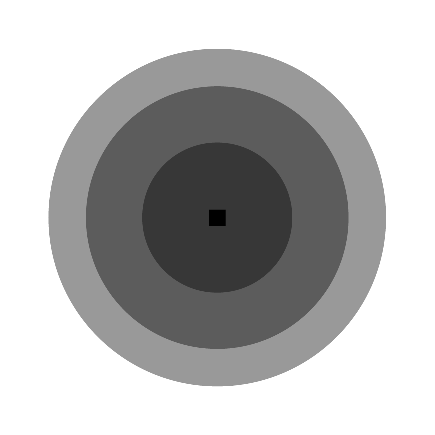
\includegraphics{kapitoly/img/vcones-explore.ps}}                
  \subfloat[P�i ostatn�ch akc�ch]{\label{fig:vcones-ostatni}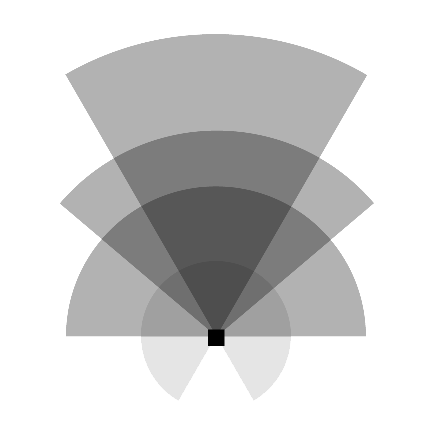
\includegraphics{kapitoly/img/vcones-normal.ps}}
  \caption{Kruhov� v�se�e ur�uj�c� agentovo vn�m�n�}
  \label{fig:vcones}
\end{figure}

Mno�ina v�se�� ur�uje agent�v zp�sob vn�m�n�. Toho jsme vyu�ili a definovali dv� r�zn� mno�iny kruhov�ch v�se��.
Jednu pro chv�le kdy se agent rozhl�� (atomick� akce Explore \ref{fig:vcones-explore}) a jednu pro zbyl� p��pady \ref{fig:vcones-ostatni}.
�hel 360� v prvn�m p��pad� simuluje to, �e p�i rozhl�en� se agent postupn� pod�v� do v�ech stran.
\\

Viditeln� p�edm�ty projdou filtrem pozornosti, kde je upravena jejich aktu�ln� atraktivita. Atraktivita p�edm�tu m� dv� slo�ky, statickou a dynamickou.
Dynamick� atraktivita z�le�� na atomick� akc� a �innosti, kterou agent pr�v� prov�d�, nab�v� hodnot 0..1, viz tabulka.
Aktu�ln� atraktivita p�edm�tu je sou�in statick� a dynamick� atraktivity a jejich viditelnosti.
\\

Pokud je fantom p�edm�tu ji� v percep�n�m poli, intenzita fantomu stoupne o aktu�ln� atraktivitu p�edm�tu.
Pokud nen�, je vytvo�en nov� fantom a p�id�n do percep�n�ho pole s intenzitou odpov�daj�c� aktu�ln� atraktivi� p�edm�tu.
P�id�n� fantomu v�ak nen� propagov�no hned d�le (nap�. do prostorov� mapy).
Kdy� jsou zpracov�ny v�echny p�edm�ty, kter� agent tento krok vid�l, jsou fantomy v percep�n�m poli se�azeny dle intenzity.
Pokud je fantom� v�ce ne� velikost percep�n�ho pole (PARAM), jsou fantomy s nejni��� intenzitou z pole odstran�ny.
Teprve nyn� jsou nov� p�idan� fantomy p�ed�ny prostorov� map� a procesn� ��sti (pouze ty, kter� se ve�ly do percep�n�ho pole).
\\

\chapter{Model prostorov� mapy} \label{chapter-model}

Agent popsan� v p�edchoz� kapitole m� dlouhodobou pam�, kter� obsahuje pouze prostorovou mapu.
Tu je mo�n� rozd�lit na dv� logick�ch ��st�: \emph{pam�t na p�edm�ty} a \emph{vrstva uzl�}.
\\

Vrstva uzl� �e�� rozlo�en� uzl� v prostoru, tedy pokryt� sv�ta uzly, kter� imituj� place cells.
M� za �kol m�nit hustotu uzl� dle zm�n sv�ta a vytv��et jejich hiearchii.
Pam� na p�edm�ty vyu��v� t�chto uzl� k ukl�d�n� informac� o poloze p�edm�t�\footnote{Vrstvu uzl� lze tak ch�pat jako pod��zenou pam�ti na p�edm�ty.}.
\\

Zat�mco pam� na p�edm�ty je nez�visl� na velikosti sv�ta, vrstva uzl� je navr�ena pro jeden uzav�en� prostor.
Z�rove� je pam� na p�edm�ty nez�visl� na  konkr�tn�ch mechanismech vrstvy uzl� a obr�cen�.
V�sledkem je, �e architekturu jedn� ��sti lze zm�nit bez z�sahu do architektury druh� ��sti.
Druh�m v�sledkem je, �e model lze snadno roz���it pro sv�ty v�t�� ne� jeden uzav�en� prostor, pokud agent bude zn�t topologii sv�ta.
Toto roz���en� je podrobn�ji pops�no v kapitole \ref{chapter-complex-space}.
\\

N�sleduj�c� dv� podkapitoly podrobn�ji popisuj� \emph{pam� na p�edm�ty} a \emph{vrstvu uzl�}.
V dal��ch dvou podkapitol�ch jsou p�edstaveny dva modely vrstvy uzl�, kter� jsme postupn� navrhli.
\\
\section{Pam�t na p�edm�ty}

Pam� na p�edm�ty �e�� ukl�d�n� objekt� (a potencion�ln� dal��ch informac�) k uzl�m.
Tedy ukl�d� informace typu "objekt XY je v uzlu n42 s intenzitou 5,2". Pam� na p�edm�ty vych�z� z pr�ce Tom�e Korenka [literatura-korenko].
\\

Pam� nepracuje p��mo s re�ln�mi p�edm�ty, ale vytv��� si jejich kopie, pam�ov� stopy p�edm�t�.
Pro ka�d� re�ln� p�edm�t m� pam� nejv��e jednu pam�ovou stopu.
Ta m� odkaz na re�ln� p�edm�t, kter� uchov�v� a intenzitu ur�uj�c�, jak moc si agent dan� p�edm�t pamatuje.
\\

Mezi pam�ov�mi stopami p�edm�t� a uzly mapy je asociativn� s�, kter� se vytv��� v pr�b�hu simulace, dle toho, jak agent vn�m� p�edm�ty kolem sebe.
Pam�ti je v ka�d�m kroku p�edlo�ena mno�ina vjem� (m��e b�t pr�zdn�).
Vjem je trojice (p�edm�t, poloha, intenzita).
Vjem m� sv�j typ, dan� ud�lost�, kterou byl vyvol�n, jejich p�ehled je v tabulce \ref{tab:typy-vjemu}.
Ka�d� typ m� ur�en� koeficient, kter�m je vyn�sobena intenzita vjemu p�ed jeho zpracov�n�m prostorovou mapou, tyto koeficienty jsou parametry modelu.
\\


\begin{table}[h!]
\begin{center}
\begin{tabular}{|l|p{6cm}|}\hline
ObjectNoticed & agent vid� p�edm�t, kter� minul� krok simulace nevid�l \\
\hline
ObjectNoticedAgain & agent vid� p�edm�t, kter� vid�l ji� p�edchoz� krok simulace \\
\hline
ObjectFound & agent nalezl p�edm�t jako v�sledek chytr� akce LookUpInMemory \\
\hline
ObjectNotFound & agent nenalezl p�edm�t tam, kde ho hledal p�i chytr� akce LookUpInMemory \\
\hline
ObjectUsed & agent pou�il p�edm�t k proveden� �innosti \\
\hline
\end{tabular}\\
\end{center}
\centering
\caption{Atomick� akce}
\label{tab:typy-vjemu}
\end{table}


Proces zpracov�n� vjemu prostorovou mapou je shrnut v \ref{alg:zpracovani-vjemu} zpracov�n� vjemu.
V prvn�m kroku je ur�ena pam�ov� stopa uchov�vaj�c� informaci o p�edm�tu. Pokud nen� nalezena, je vytvo�ena.
V kroku 4 je ur�ena intenzita o kterou bude zv��ena vazba mezi pam�ovou stopou a uzlem dle vzorce vvv.
\\


\begin{algorithm}[h!]
\caption{Zpracov�n� vjemu}
\label{alg:zpracovani-vjemu}
\begin{algorithmic}[1]
\State ur�en� pam�ov� stopy p�edm�tu
\State zv��en� intenzity pam�ov� stopy o intenzitu vjemu
\State $nodes\gets$ v�echny uzly, do jejich� okol� vjem padl
\ForAll{$n \in nodes$}
	\State intenzita($n$) $\gets$ dle vzorce vvv
	\State zv��en� intenzity vazby mezi pam�ovou stopou a uzlem n
\EndFor
\State vjem je p�ed�n vrstv� uzl� k dal��mu zpracov�n�
\end{algorithmic}
\end{algorithm}


��st tohoto procesu m��e b�t prov�d�na v r�mci vrstvy uzl�, nap�. v modelu Energy Layer.
\\

Prostorov� mapa je schopna ��ci, kde se nach�zej� p�edm�ty, kter� agent p�ed t�m vid�l. Tato informace je ulo�ena v d��ve zm�n�n� asociativn� s�ti.
��m bl�e je p�edm�t n�jak�mu uzlu mapy, t�m vy��� je intenzita vazby mezi nimi.
Kdy� agent hled� p�edm�t maj�c� n�jakou affordanci, provede se proces popsan� v \ref{alg:vzpomenuti}. V kroku 2 je spo��t�na poloha p�edm�tu z informac� ulo�en�ch v asociativn� s�ti.
Poloha p�edm�tu je v�en� centroid v�ech uzl�, kter� maj� vazbu na pam�ovou stopu, v�hou je intenzita vazeb.
\\

\begin{algorithm}[h!]
\caption{Vzpomenut� si na p�edm�t}
\label{alg:vzpomenuti}
\begin{algorithmic}[1]
\State Vybr�n� pam�ov� stopy s nejvy��� intenzitou, kter� m� po�adovanou affordanci
\State Aktualizace informace o poloze p�edm�tu v pam�ov� stop�
\State Pam�ov� stopa je p�ed�na pam�ov� ��sti kr�tkodob� pam�ti, kter� z n� vytvo�� pam�ov�ho fantoma
\end{algorithmic}
\end{algorithm}


\begin{enumerate}
\item item
\end{enumerate}

\section{Vrstva uzl�}

Vrstva uzl� je ��st prostorov� mapy zodpov�dn� za rozlo�en� uzl� v prostoru, zm�nu jejich rozlo�en�.
D�le obsahuje mechanismy pro zm�nu po�tu uzl� a vytv��en� hiearchie.
\\

\begin{definition}[Okam�it� napln�nost uzlu]
Uzel prostorov� mapy m� vazby na pam�ov� stopy. Tyto vazby maj� intenzitu.
Okam�it� napln�nost uzlu je sou�et intenzit v�ech vazeb uzlu na pam�ov� stopy.
P�edstavuje m�ru nau�enosti uzlu, resp. m�ru jeho d�le�itosti pro pam� na p�edm�ty.
��m v�ce pam�ov�ch stop vyu��v� uzel a ��m intenzivn�j�� jsou, t�m m�n� by se m�la m�nit jeho poloha.
\end{definition}

Okam�it� napln�nost uzlu z�vis� p��mo na vazb�ch na pam�ov� stopy.
Kdy� kles� jejich intenzita, kles� stejn� i okam�it� napln�nost.
Nen� tedy mo�n� model dostate�n� parametrizovat, tak aby okam�it� napln�nost uzlu klesala rychleji �i pomaleji, ne� intenzita vazeb.
\\

\begin{definition}[Rychlost kles�n� napln�nosti]
Parametr modelu \param{rychlost kles�n� napln�nosti} uzlu ur�uje, jak rychle bude napln�nost uzlu klesat.
\end{definition}

\begin{definition}[Napln�nost uzlu]
Napln�nost je vlastnost uzlu, kter� z�le�� p��mo na \emph{okam�it� napln�nosti uzlu}, nem�n� se v�ak tak rychle, m� ur�itou pam�.
Napln�nost uzlu $node$ budeme d�le ve vzorc�ch ozna�ovat znakem $\mu(node)$.
\end{definition}

P�i vytvo�en� nov�ho uzlu je jeho napln�nost rovna nule. V pr�b�hu simulace se m�n�, kdykoli je zv��ena intenzita vazby
mezi uzlem a pam�ovou stopou, je stejn� zv��ena i napln�nost uzlu.
V ka�d�m kroku simulace je napln�nost uzlu sn�ena o parametr \param{rychlost kles�n� napln�nosti}, nem��e ale klesnout pod nulu.
\\
\section{Model zalo�en� na Kohonenov� map�}

V�t�ina model� pam�ti, zm�n�n�ch v t�et� kapitole, vyu��v� samoorganiza�n� Kohonenovy mapy \cite{litKohonen}.
Kohonenova mapa je model neuronov� s�t� u��c� se bez u�itele, vyu��v� sout�n� strategii u�en�.
Neurony jsou v Kohonenov� map� uspo��d�ny do topologick� struktury, nej�ast�ji do dvourozm�rn� m��ky.
T�m je ur�eno, jak� neurony spolu soused�.
Okol�m neuronu $N_s(c)$ velikosti $s$ neuronu $c$ pak rozum�me jeho sousedy a dal�� neurony, jejich� vzd�lenost v topologii je men�� ne� $s$:

\begin{equation} 
N_s(c) = \{j:d(j,c)\leq s\},
\label{formula:km-okoli}
\end{equation}

kde $d(j,c)$ je vzd�lenost v topologick� struktu�e.
Neurony Kohonenovy mapy p�i u�en� sout�� o to, kter� z nich bude aktivn� p�i dan�m vstupu.
V�t�zn�m neuronem se stane ten, kter� se nejv�ce podob� vstupu. Jeho v�ha a v�hy neuron� v jeho okol� jsou upraveny.
Ostatn� neurony jsou neaktivn� a neu�� se. Kohonenova mapa a dal�� modely samoorganiza�n�ch map jsou pops�ny nap�. v \cite{litSimaNeruda}.
\\

\begin{figure}[h!]
  \centering
  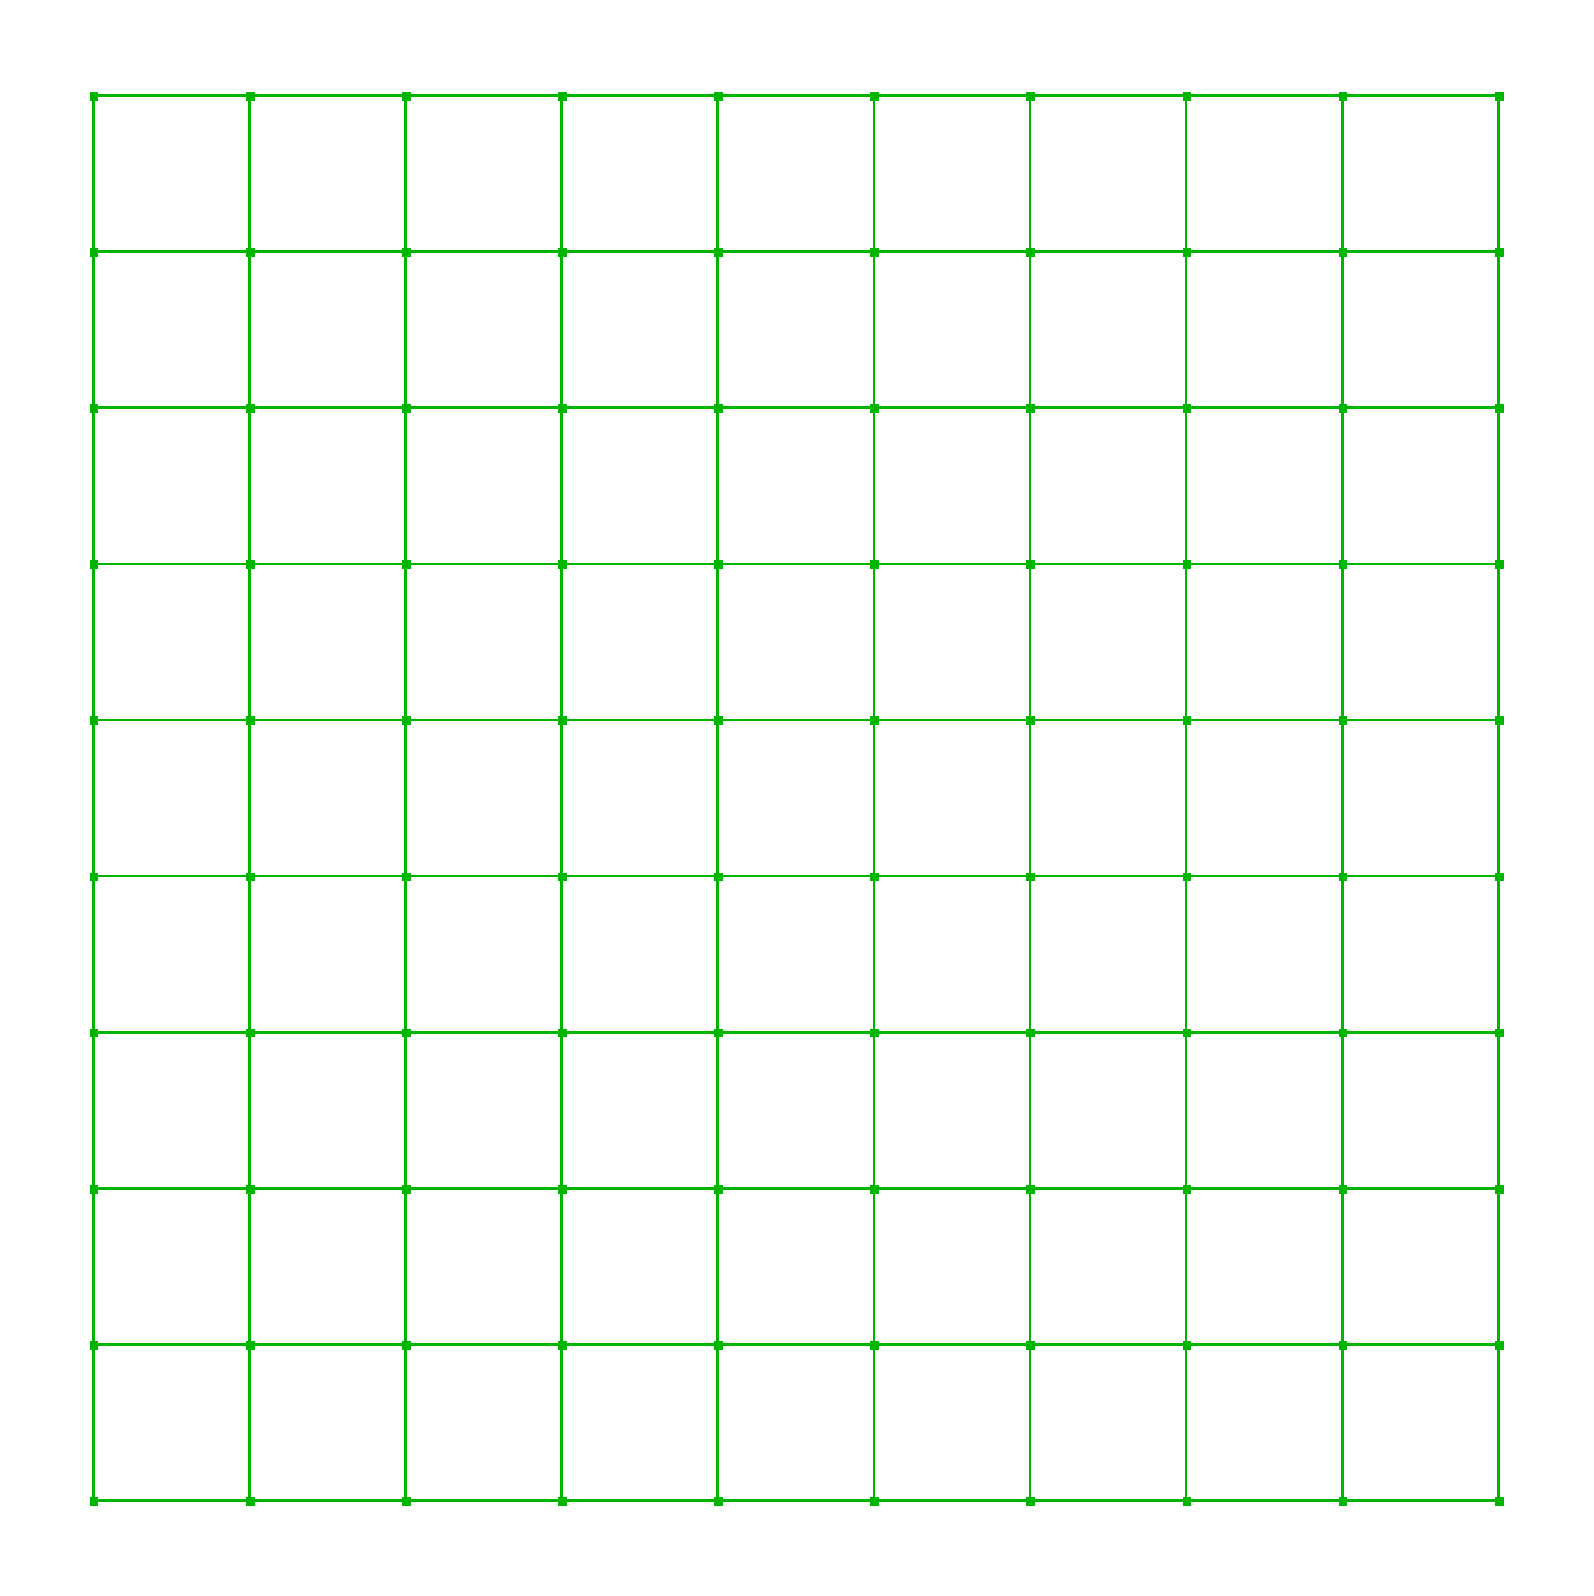
\includegraphics[width=0.5\textwidth]{img/kml/kml-start-grid.eps}
  \caption{Po��te�n� pokryt� sv�ta uzly uspo��dan�mi do �tvercov� m��ky.}
  \label{fig:kml-start}
\end{figure}

Kohonenova mapa by m�la spl�ovat na�e po�adavky. Um� rozm�stit uzly do hustoty odpov�daj�c� rozm�st�n� p�edm�t� v prostoru.
Um� se u�it online, ka�d� vjem agenta je mo�n� ch�pat jako prvek tr�novac� mno�iny dat.
Navrhli jsme tedy model vrstvy uzl� zalo�en� na Kohonenov� map�.
\\

\begin{definition}[Koeficient u�en�]
Rychlost u�en� Kohonenovy mapy je parametrizovateln�. Navr�en� model toho vyu��v�, koeficient u�en� ur�uje tuto rychlost.
\end{definition}


Na za��tku je prostor pokryt Kohonenovou mapou, uzly jsou uspo��d�ny do �tvercov� m��ky, viz obr�zek \ref{fig:kml-start}.
Poka�d�, kdy� je vjem p�ed�n ke zpracov�n�, provede se tr�nov�n� Kohonenovy mapy dle algoritmu \ref{alg:km-uceni}.
\\


\begin{algorithm}[h!]
\caption{Zpracov�n� vjemu}
\label{alg:km-uceni}
\begin{algorithmic}[1]
\State $node_{win} \gets$ vyhr�vaj�c� uzel (nejbli��� k poloze vjemu)
%\State $queue \gets \emptyset$
\State $queue \gets \{node_{win}\}$
\While{$queue\not= \emptyset$}
	\State $n \gets first(queue)$
	\State $queue \gets queue  \setminus \{n\}$
	\State zm�na polohy $n$ dle vzorce \ref{formula:km-uceni} \label{alg:km-uceni-vzorec}
	\State $queue \gets$ sousedi $n$ (pokud nebyli je�t� tr�nov�ni)
\EndWhile
\State vjem je p�ed�n vrstv� uzl� k dal��mu zpracov�n�
\end{algorithmic}
\end{algorithm}

Vyhr�vaj�c� uzel $node_{win}$ je ur�en dle vzd�lenosti mezi uzlem a vjemem:
\begin{equation}
node_{win} =\argmin_{node \in nodes} dist(node,vjem).
\end{equation}

V algoritmu je na ��dce \ref{alg:km-uceni-vzorec} zm�n�na poloha uzlu mapy. Uzel je posunut sm�rem k poloze vjemu o \(\Delta xy(n, vjem)\) dle vzorce:

\begin{equation} 
\Delta xy(n, vjem) = coef_{neighbour}(n, node) \times coef_{learn} \times dist(n, vjem),
\label{formula:km-uceni}
\end{equation}

kde \(coef_{neighbour}\) je vzd�lenost mezi vyhr�vaj�c�m uzlem a pr�v� tr�novan�m uzlem v Kohonenov� map�
 a \(coef_{learn}\) je koeficient u�en� Kohonenovy mapy.
Vzorec \eqref{formula:km-uceni} je analogi� u�en� Kohonenovy mapy.
\\

T�mto algoritmem by se m�la prostorov� mapa v pr�b�hu simulace nau�it rozm�st�n� p�edm�t� ve sv�t� a p�izp�sobit se mu.
Uzly mapy se postupn� p�esunou do m�st s velkou �etnost� vjem� a rozm�st�n� uzl� by se tak m�lo v �ase postupn� bl�it rozm�st�n� p�edm�t�.
\\

\begin{figure}[h!]
  \centering
  \subfloat[Po 1000 kroc�ch]{\label{fig:kml-preuceni-1}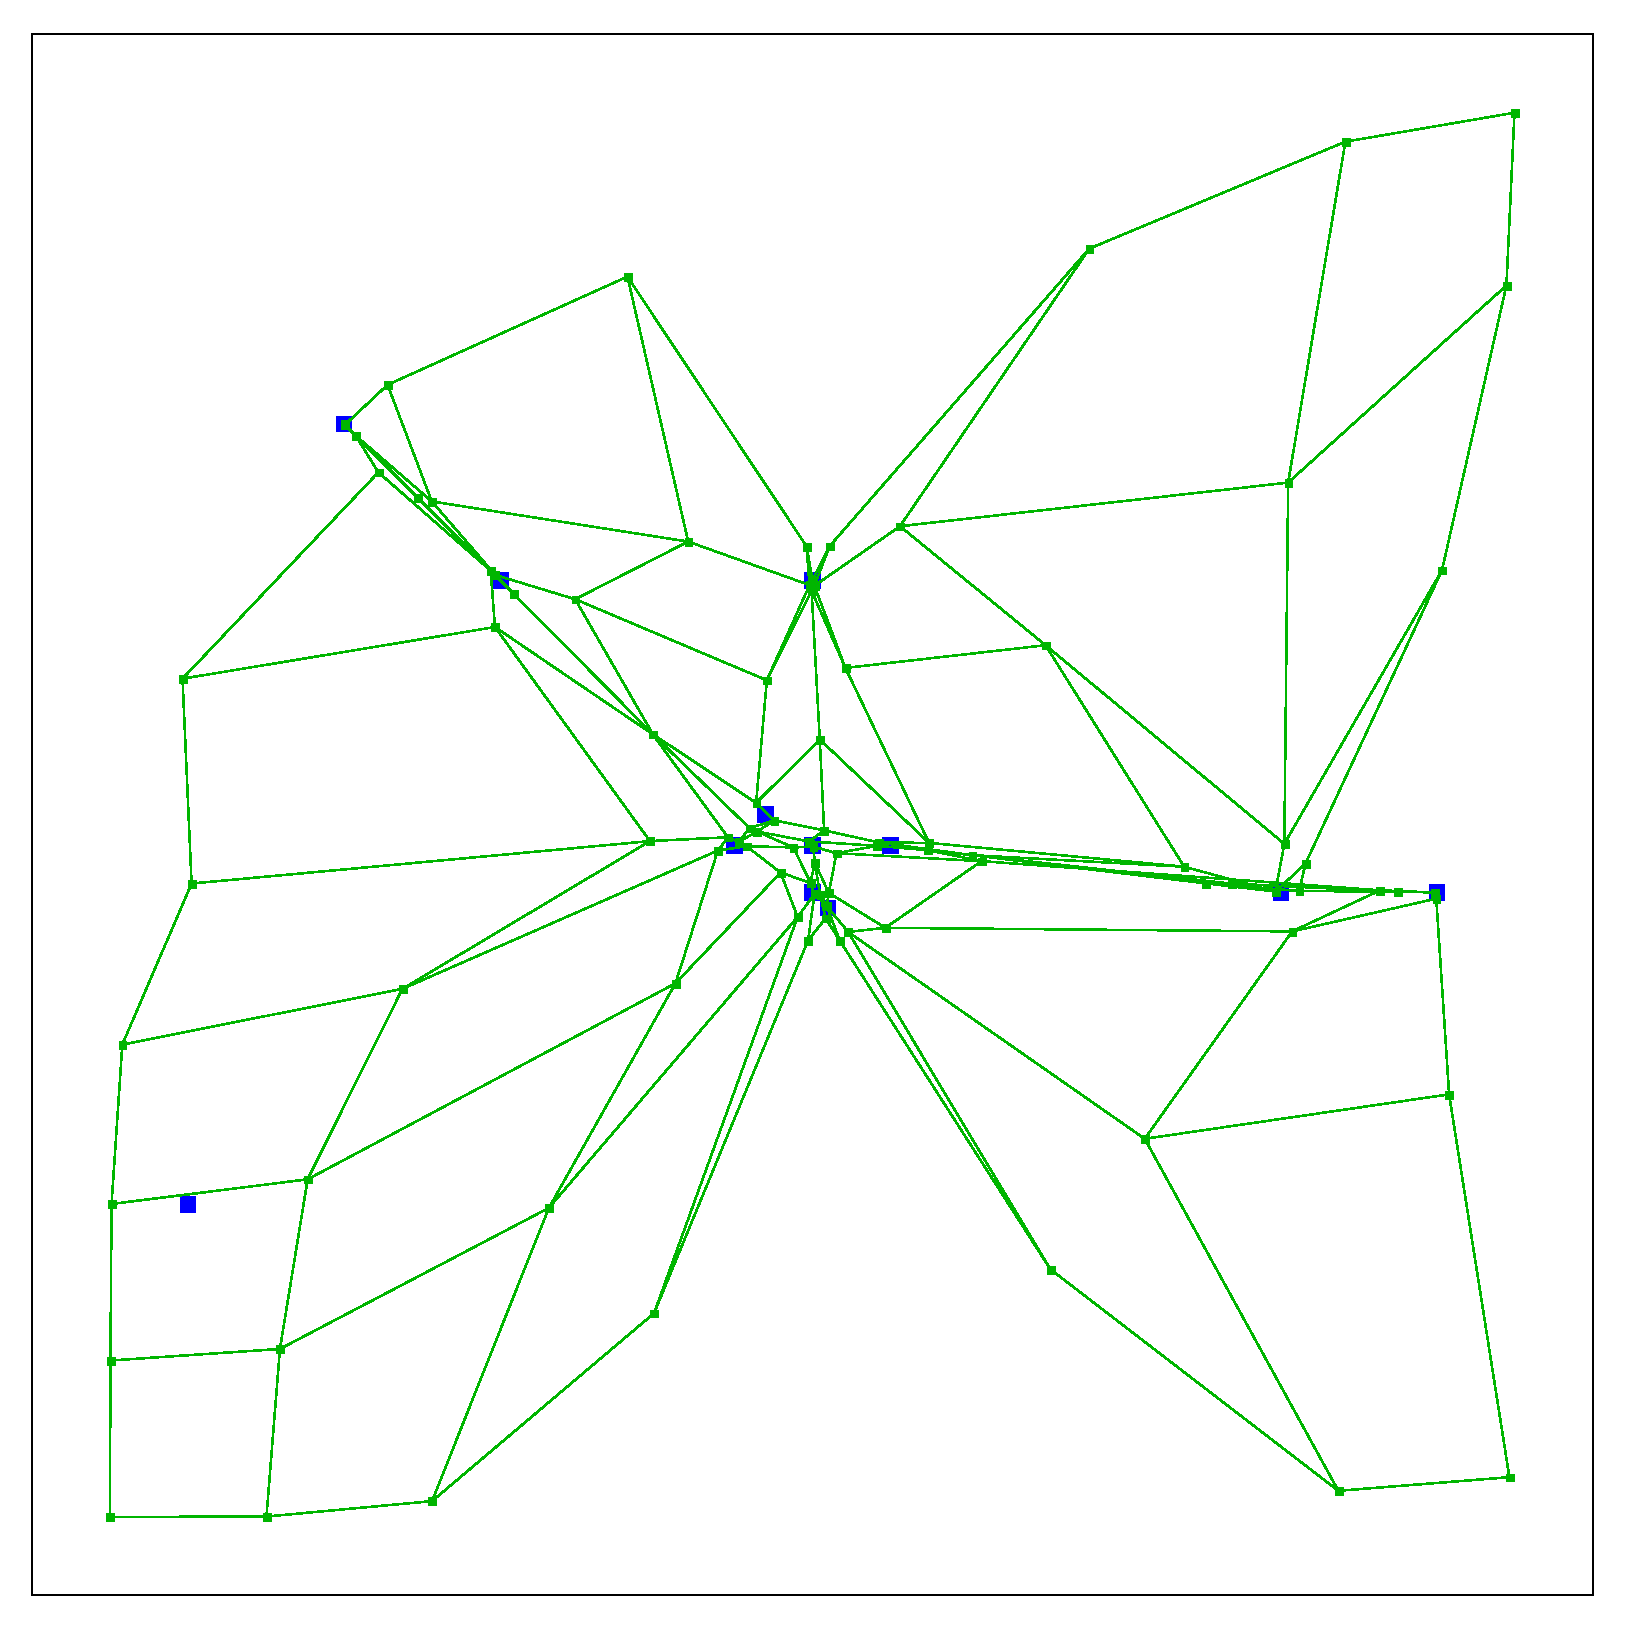
\includegraphics[width=0.5\textwidth]{img/kml/kml-preuceni-1.eps}}
  \subfloat[Po 4000 kroc�ch]{\label{fig:kml-preuceni-2}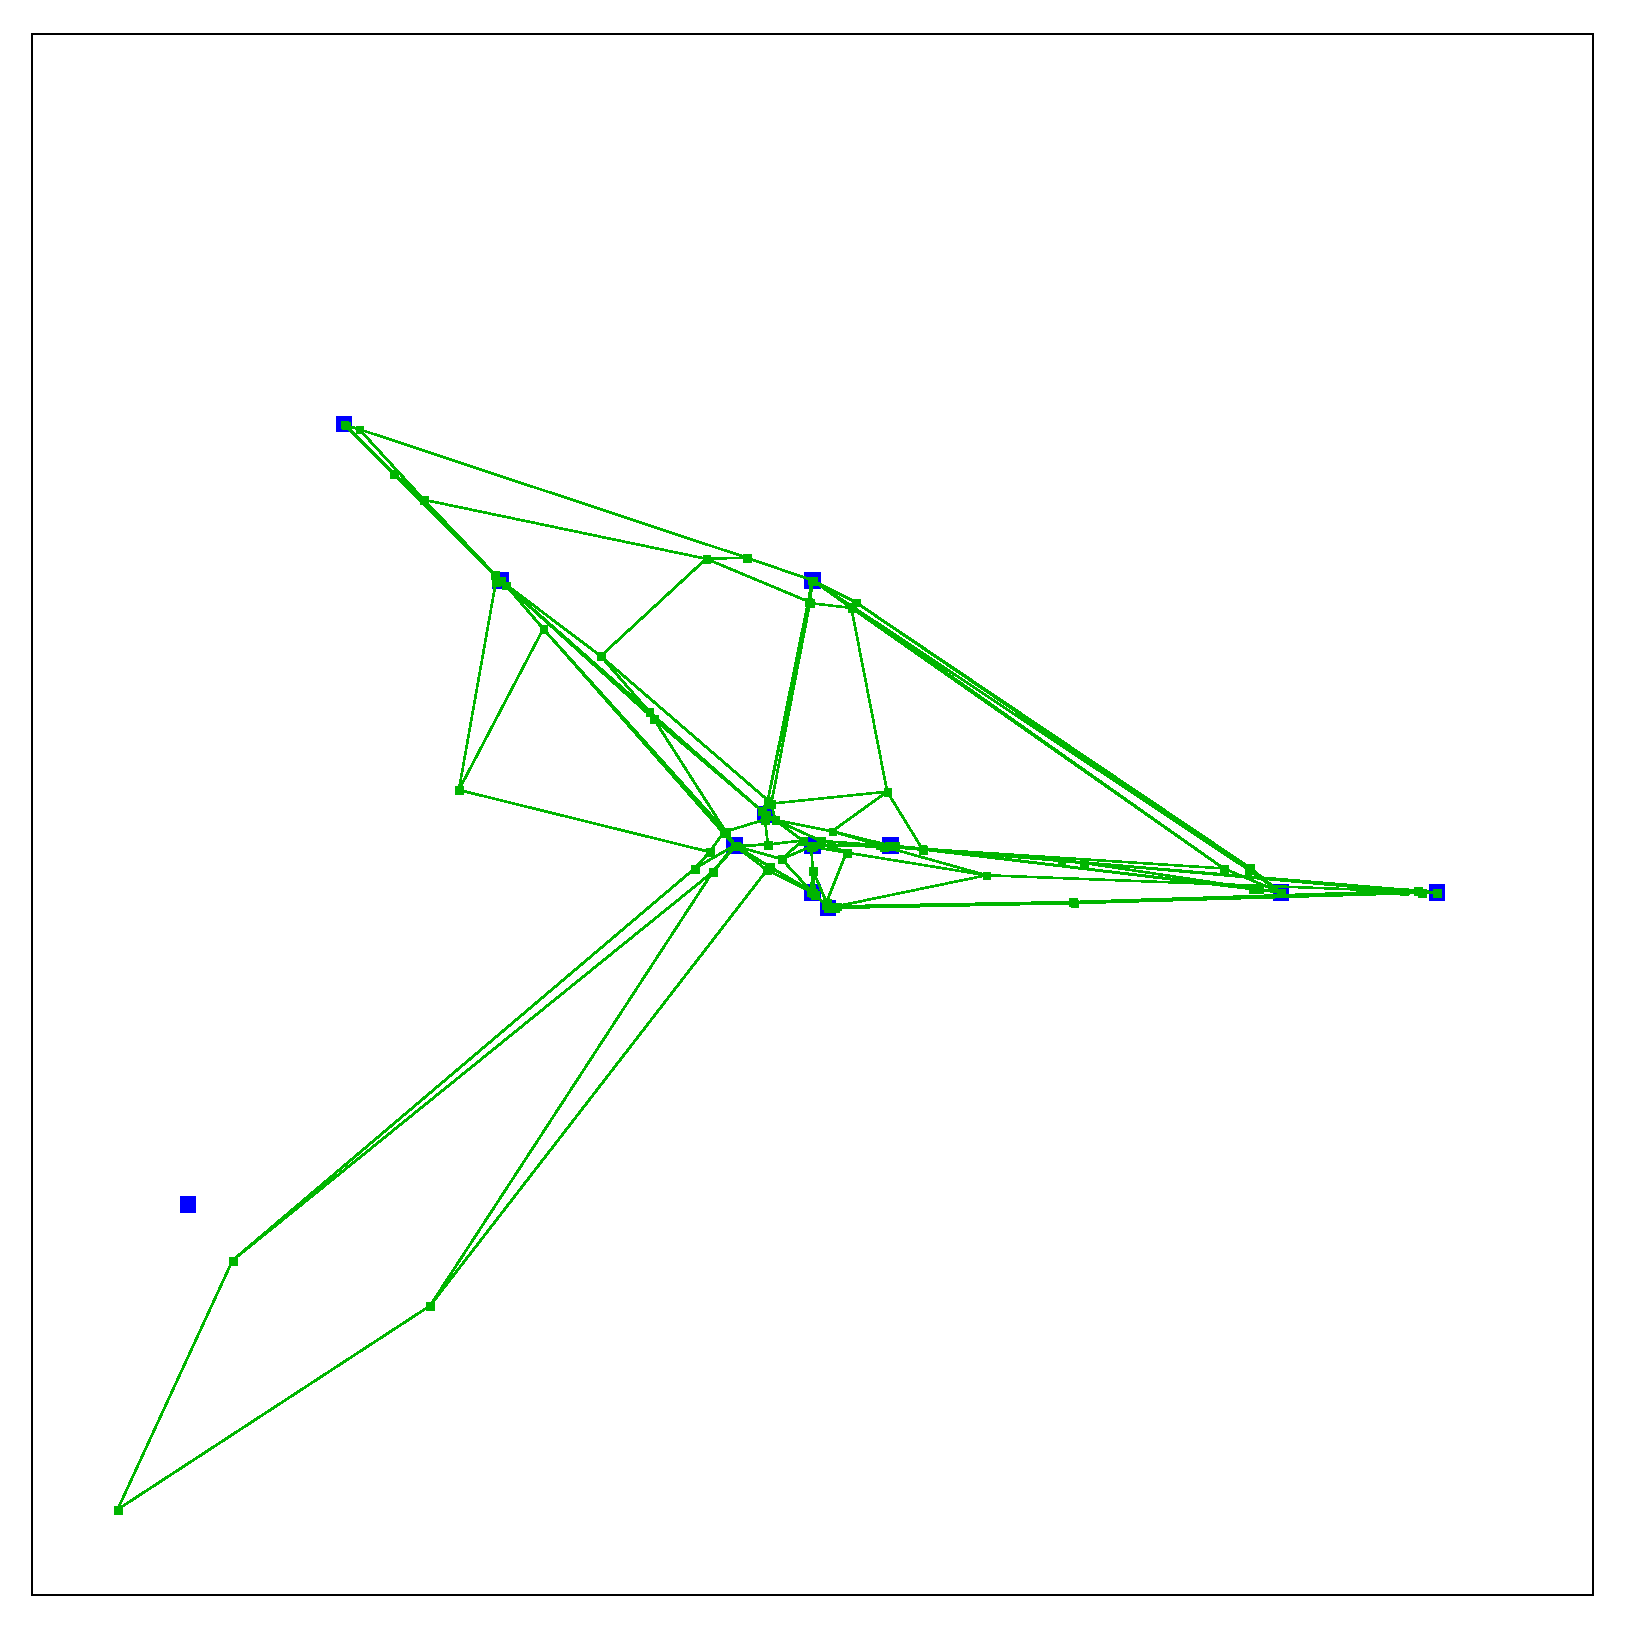
\includegraphics[width=0.5\textwidth]{img/kml/kml-preuceni-2.eps}}
  \caption{Test modelu a uk�zka jeho p�eu�en�}
  \label{fig:kml-preuceni}
\end{figure}

Test modelu (obr�zek \ref{fig:kml-preuceni}) uk�zal, �e k tomu skute�n� dojde, ale v�ce, ne� bychom cht�li.
Probl�m, kter� nastal je, �e se s� pro na�e pot�eby \uv{p�eu�ila}
 -- uzly se �asem v�echny p�esunuly k p�edm�t�m a prostor bez p�edm�t� z�stal pr�zdn�, bez uzl�.
Navrhli jsme dv� �e�en�:
\begin{CompactItemize}
\item Um�l� p�edm�ty - p�id�n� um�l�ch p�edm�t�, kter� se budou sna�it dr�et p�vodn� rozlo�en� uzl� Kohonenovy mapy
\item Odpudivost uzl� - uzly mapy se budou vz�jemn� odpuzovat, aby se nenahromadily v�echny v jednom m�st�
\end{CompactItemize}

V��e zm�n�n� �e�en� jsme vyzkou�eli v jednoduch� �tvercov� m�stnosti.
\\

\subsection{Um�l� p�edm�ty}
Toto �e�en� p�id�v� do sv�ta dal�� p�edm�ty, agent je nevyu��v� k pln�n� sv�ch z�m�r�, pouze je vn�m� a m�n� dle nich svou prostorovou mapu.
Um�l� p�edm�ty mus� m�t ni��� atraktivitu ne� re�ln� p�edm�ty, aby nem�ly na prostorovou mapu v�t�� vliv ne� opravdov� p�edm�ty.
\\

Um�l� p�edm�ty jsou do sv�ta p�id�ny na za��tku, p�i vytv��en� �tvercov� s�t�. V ka�d�m m�st�, kde je uzel s�t�, je vytvo�en jeden um�l� p�edm�t.
Agent je bude vn�mat stejn� jako ostatn� p�edm�ty, v pr�b�hu simulace budou k sob� p�itahovat uzly s�t� stejn� jako re�ln� p�edm�ty.
T�m by m�ly udr�et Kohonenovu mapu rozta�enou i v m�stech, kde re�ln� p�edm�ty nejsou.
\\

\begin{figure}[h!]
  \centering
  \subfloat[Po 500 kroc�ch]{\label{fig:kml-bo-1}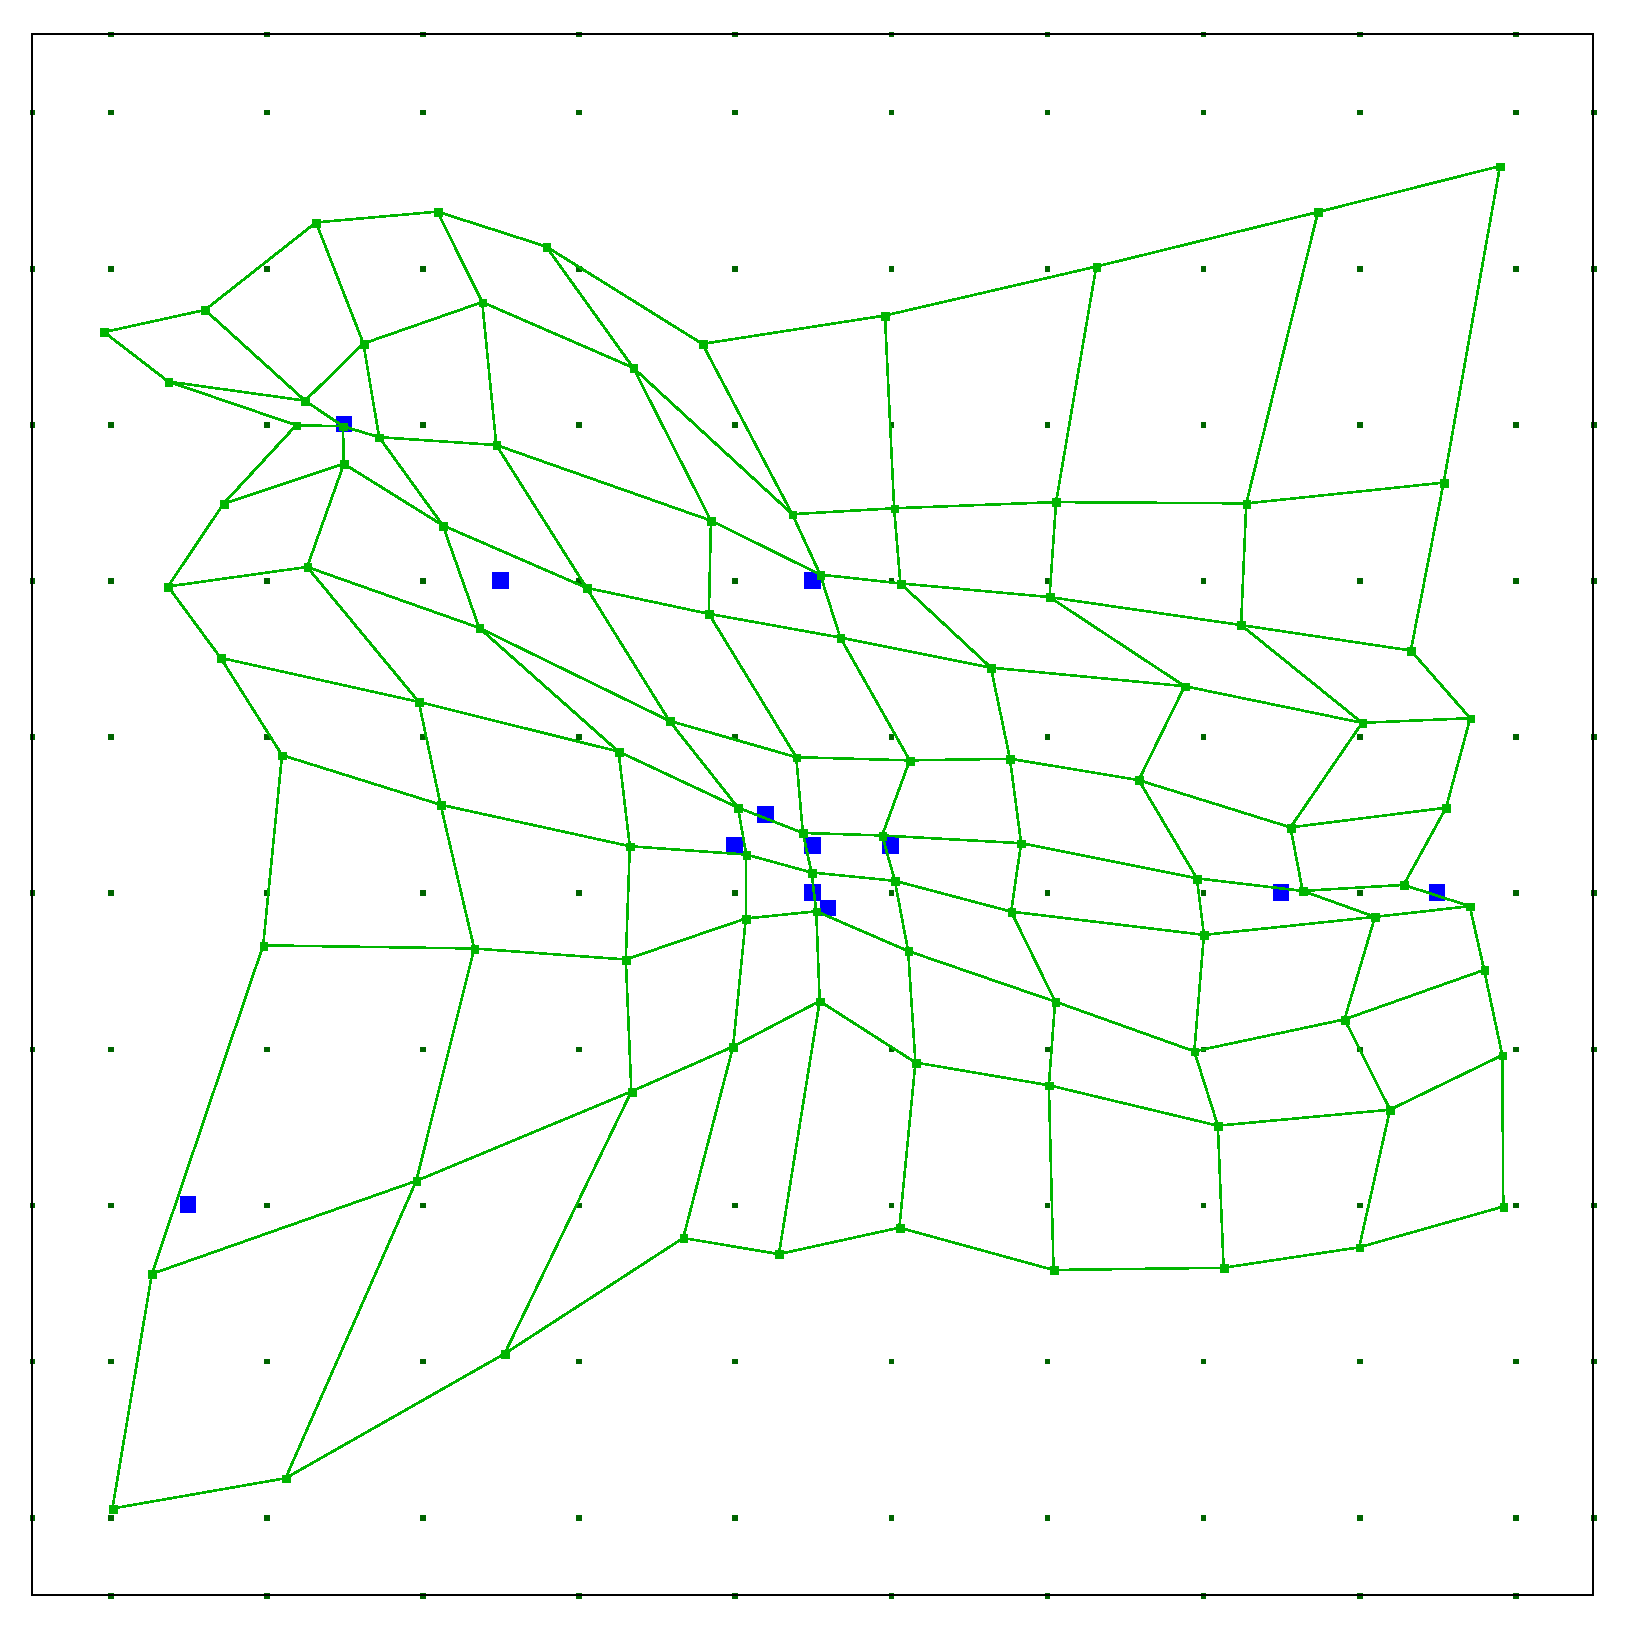
\includegraphics[width=0.5\textwidth]{img/kml/bo-0.5-0500.eps}}
  \subfloat[Po 1000 kroc�ch]{\label{fig:kml-bo-2}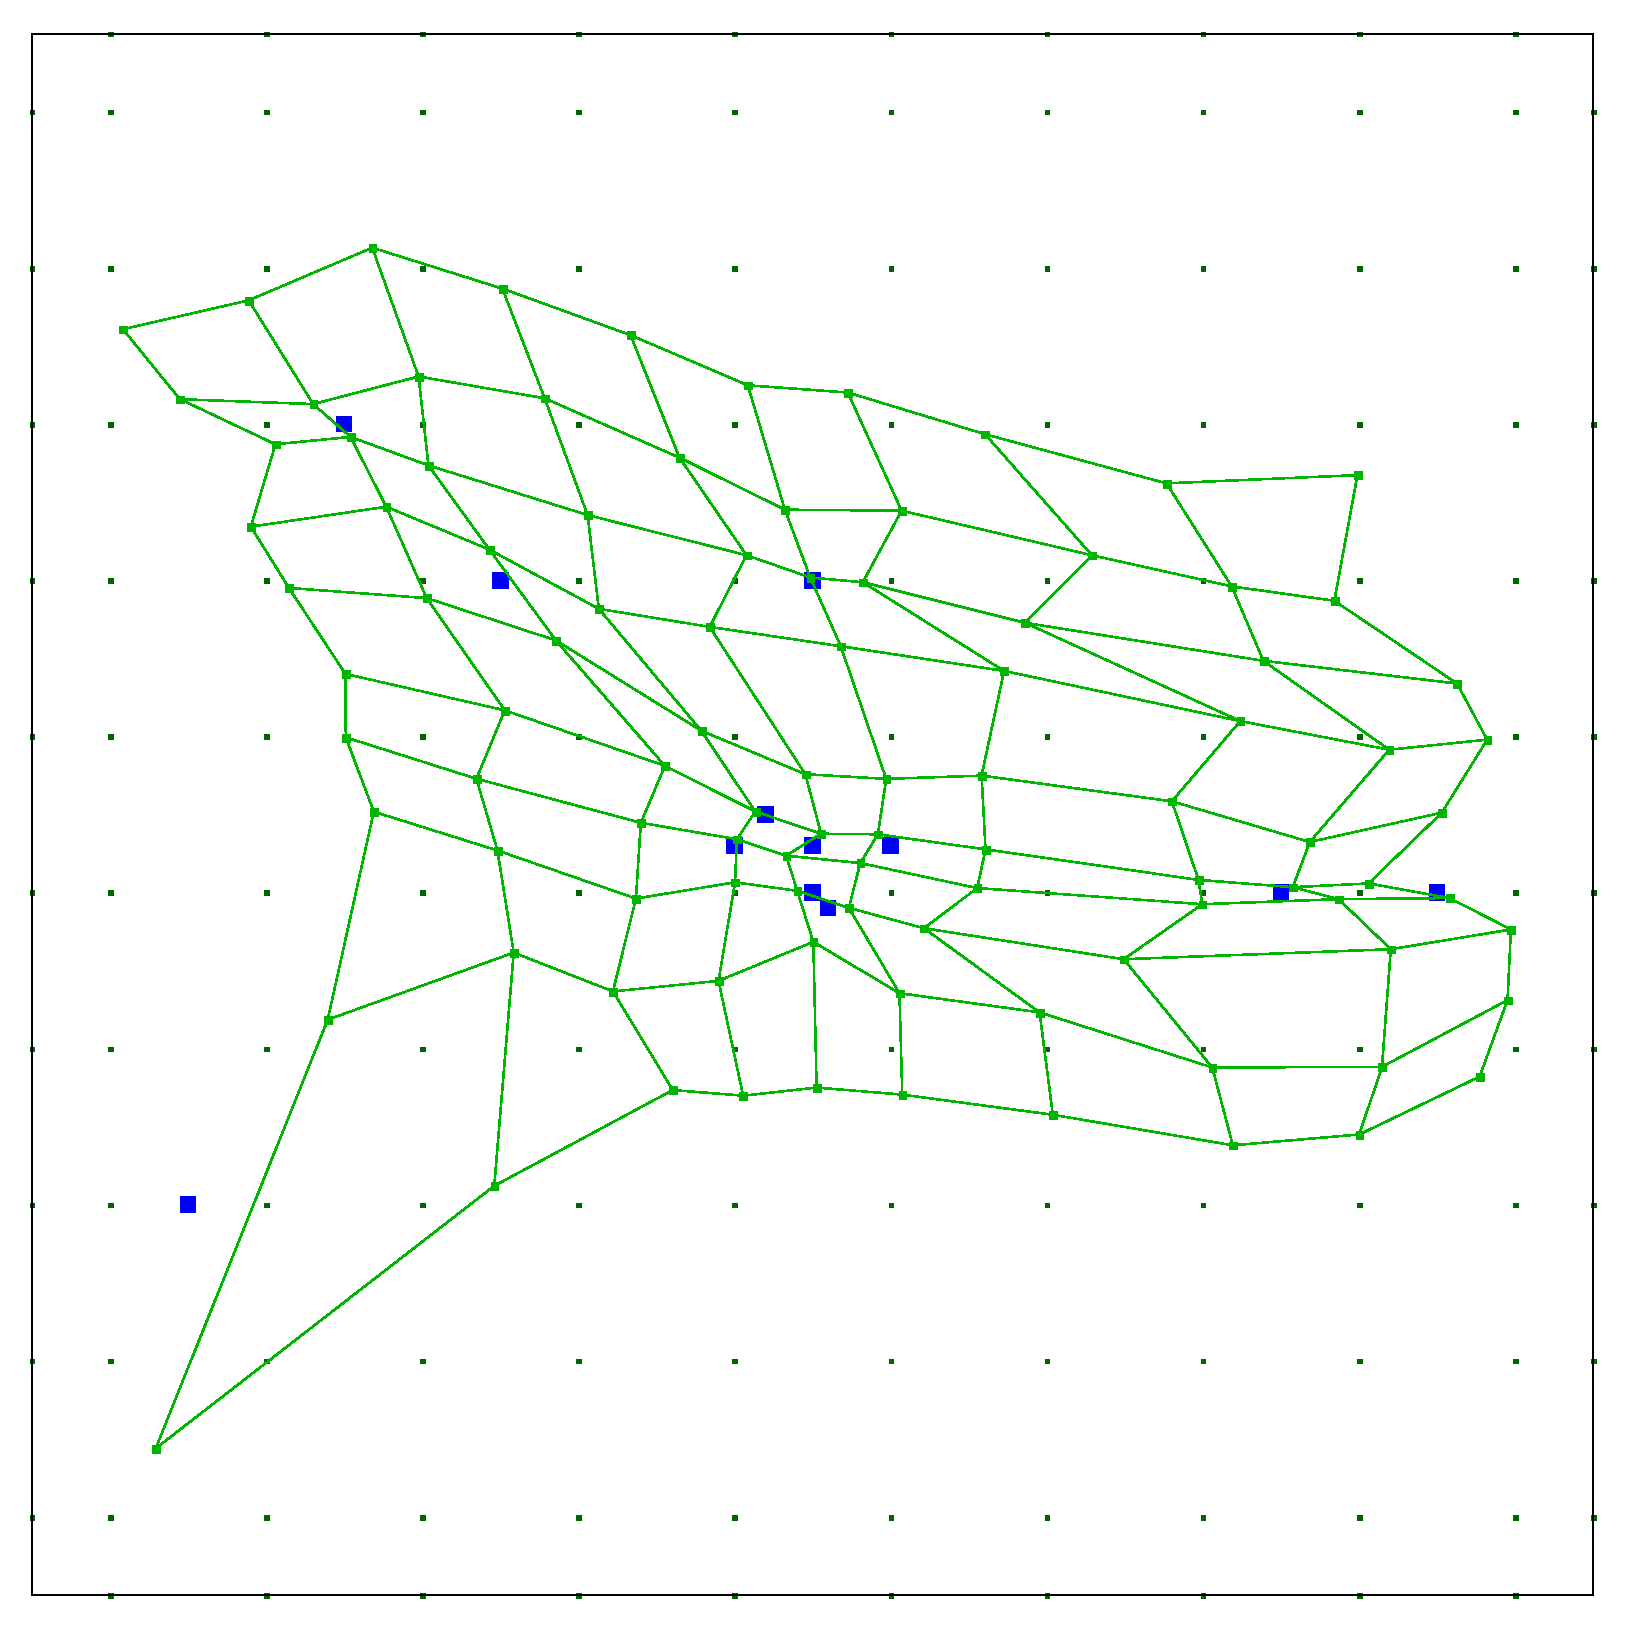
\includegraphics[width=0.5\textwidth]{img/kml/bo-0.5-1000.eps}}
  \caption{Test modelu s um�l�mi p�edm�ty}
  \label{fig:kml-baseobjs}
\end{figure}

V�sledek testu je na obr�zku \ref{fig:kml-baseobjs}\footnote{Dal�� v�sledky test� s r�znou hodnotou atraktivity um�l�ch p�edm�t� jsou na p�ilo�en�m DVD.}.
Uzly mapy se v pr�b�hu simulace stahuj� do st�edu m�stnosti.
Mapa se stahuje do st�edu m�stnosti bez ohledu na vliv um�l�ch p�edm�t�.
D�vodem je to, �e t�i�t� v�ech um�l�ch p�edm�t� je ve st�edu m�stnosti.
Tomu bychom mohli zabr�nit zv��en�m atraktivity um�l�ch p�edm�t�, kter� jsou na kraji m�stnosti.
Jednoduch�m protip��kladem takov�ho �e�en� je m�stnost, kter� bude m�t objekty pouze na kraji (na zdech, v roz�ch).
Pak bychom pot�ebovali zv��it atraktivitu um�l�ch p�edm�t� uprost�ed m�stnosti resp. obecn� bychom museli zv��it atraktivitu um�l�ch p�edm�t� v m�stech,
kde nejsou re�ln� p�edm�ty.
T�m jsme p�evedli p�vodn� probl�m hled�n� oblast� s vy���m po�tem p�edm�t� na probl�m opa�n�, tj. na hled�n� oblast� bez p�edm�t�.
�e�en� s pou�it�m um�l�ch p�edm�t� tedy nevyhovuje.
\\

\subsection{Odpudivost uzl�} \label{s:km-odpudivost}
Do modelu jsme p�idali vz�jemnou odpudivost uzl� s�t�. V ka�d�m kroku simulace se uzly, kter� jsou p��li� bl�zko u sebe, odpuzuj�.

\begin{definition}[S�la odpudivosti]
Parametr modelu \param{s�la odpudivosti} ur�uje m�ru s jakou se budou uzly odpuzovat.
\end{definition}


Vz�jemn� odpudivost dvou uzl� z�vis� na \param{s�le odpudivosti}, na vzd�lenosti uzl� a jejich napln�nosti.
Uzel s vysokou napln�nost� se bude nach�zet v m�st�, kde je hodn� p�edm�t�.
V takov�ch m�stech by hustota uzl� m�la b�t v�t��, a proto je nutn�, aby v takov�ch m�stech byla vz�jemn� odpudivost uzl� men��.
\\

\begin{equation} 
odpudivost(n_i, n_j) = \frac{ sila_{odpudivost} }{ dist(n_i, n_j)^2 \times \mu(n_i) \times \mu(n_j) } 
\label{formula:km-odpudivost}
\end{equation}
\\

Napln�nost uzlu lze p�i ur�ov�n� vz�jemn� odpudivosti ch�pat jako analogii k hmotnosti t�les, s t�m rozd�lem,
�e odpudivost dvou uzl� je nep��mo �m�rn� sou�inu jejich napln�nost�. Odpudivost je d�na vzorcem \eqref{formula:km-odpudivost},
kde $sila_{odpudivost}$ je parametr \param{s�la odpudivosti}.
V ka�d�m kroku simulace je spo�tena vz�jemn� odpudivost uzl�. T�m jsou ur�eny v�echny odpudiv� s�ly, kter� na uzly p�sob�.
Poloha uzl� je pak upravena dle t�chto sil:
\\

\begin{equation} 
\Delta_{xy}(node) = \frac{
\sum_{\substack{
   n \in nodes
  }}
  odpudivost(n, node)
}{ max(1, \mu(node)) }
\label{formula:el-odpudivost}.
\end{equation}
\\


\begin{figure}[h!]
  \centering
  \subfloat[Cel� m�stnost s nazna�en�m v��ezem]{\label{fig:kml-ag-cele}\includegraphics[height=0.36\textwidth]{img/kml/ag-cele.eps}}
  \quad
  \subfloat[V��ez]{\label{fig:kml-ag-vyrez}\includegraphics[height=0.36\textwidth]{img/kml/ag-vyrez.eps}}
  \caption{Test modelu s odpudivost� uzl�}
  \label{fig:kml-ag}
\end{figure}

V�sledek testu je na obr�zku \ref{fig:kml-ag}\footnote{Dal�� v�sledky test� s r�znou hodnotou s�ly odpudivosti jsou na p�ilo�en�m DVD.}.
Ukazuje, �e odpudivost skute�n� rozprost�e uzly po cel� m�stnosti.
Objevil se v�ak jin� probl�m -- odpudiv� s�ly deformuj� Kohonenovu mapu do stavu, kdy jej� n�sleduj�c� u�en� ned�v� smysl.
S� se p�ekrout� tak, �e uzly (na obr�zku \ref{fig:kml-ag} �erven� vyzna�en�), kter� jsou ve virtu�ln�m sv�t� vedle sebe, jsou v s�ti daleko od sebe a obr�cen�.
\\

D��ve zm�n�n� probl�m p�eu�en� skute�n� nastal a dv� rozd�ln� �e�en� jej nedok�zala uspokojiv� vy�e�it. Model zalo�en� na Kohonenov� map� jsme tedy zam�tli.
\\
\section{Gravita�n� model}

Inspirov�ni pou�it�m odpudivosti v p�edchoz�m modelu, rozhodli jsme se vytvo�it model zalo�en� pouze na p�ita�livosti a odpudivosti.
Tedy uzly mapy jsou p�itahov�ny k p�em�t�m a z�rove� se vz�jemn� odpuzuj�. Ob� s�ly berou v potaz napln�nost uzlu.
\\

Model d�le obsahuje my�lenku, �e i kdy� �lov�k vn�m� p�edm�ty v jeden okam�ik, ukl�d�n� do pam�ti prob�h� postupn�. 
Tato my�lenka je do modelu zapracov�na tak, �e vjem je sice dod�n prostorov� map� v jeden konkr�tn� krok simulace,
ale mapa si jej ulo�� a u�� se dle n�j n�kolik n�sleduj�c�ch krok�.
\\



\subsection{Vytvo�en� vrstvy uzl�} \label{chapter-createmap}

Na za��tku simulace si agent vytvo�� prvotn� prostorovou mapu, kter� neobsahuje ��dn� informace o p�edm�tech ani jejich rozlo�en� ve sv�t�.
Obsahuje uzly, rozm�st�n� pouze dle geometrie m�stnosti. Jejich po�et a zp�sob rozlo�en� je parametrizov�n.
\\

\begin{definition}[Hustota mapy]
Parametr modelu \param{hustota mapy} ur�uje po�et uzl�, kter� jsou do m�stnosti um�st�ny p�i vytv��en� mapy.
Pokud je po��te�n� rozlo�en� mapy pravideln� m��ka, hustota mapy ur�uje, jak daleko od sebe maj� dva uzly b�t.
Jeden uzel pak pokr�v� oblast velikosti �tverce hustoty.
\end{definition}

\begin{definition}[Po��te�n� odchylka mapy]
Parametr modelu \param{po��te�n� odchylka mapy} ur�uje zp�sob rozlo�en� po��te�n�ho uzl� v prostoru.
Uk�zalo se, �e tento parametr nem� vliv na rozlo�en� uzl� po del�� dob� simulace\footnote{To je zp�sobeno odpudivost� uzl�}.
\end{definition}

Uzly mohou b�t um�st�ny zcela n�hodn� �i pravideln� ve �tvercov� m��ce s n�hodnou odchylkou.
N�hodn� odchylka m��e b�t i nulov�, ��m� je dosa�eno pravideln�ho rozlo�en� uzl�.
Uk�zky po��te�n�ho rozlo�en� uzl� jsou na obr�zku \ref{fig:createmap}.

Pokud je rozlo�en� uzl� zcela n�hodn�, je z hustoty mapy odvozen po�et uzl� dle vzorce \eqref{formula:el-start-pocet-uzlu},
kde $obsah(mistnost)$ je obsah polygonu reprezentuj�c� m�stnost a $hustota$ je hustota mapy.

\begin{equation} 
pocet = \frac{obsah(mistnost)}{hustota^2}
\label{formula:el-start-pocet-uzlu}
\end{equation}
\\


\begin{figure}[h!]
  \centering
  \subfloat[Pravideln� m��ka]{\label{fig:createmap-grid}\includegraphics[width=0.33\textwidth]{img/createmap/nodes-start-grid.eps}}
  \subfloat[Pravideln� m��ka s odchylkou 3]{\label{fig:createmap-noise3}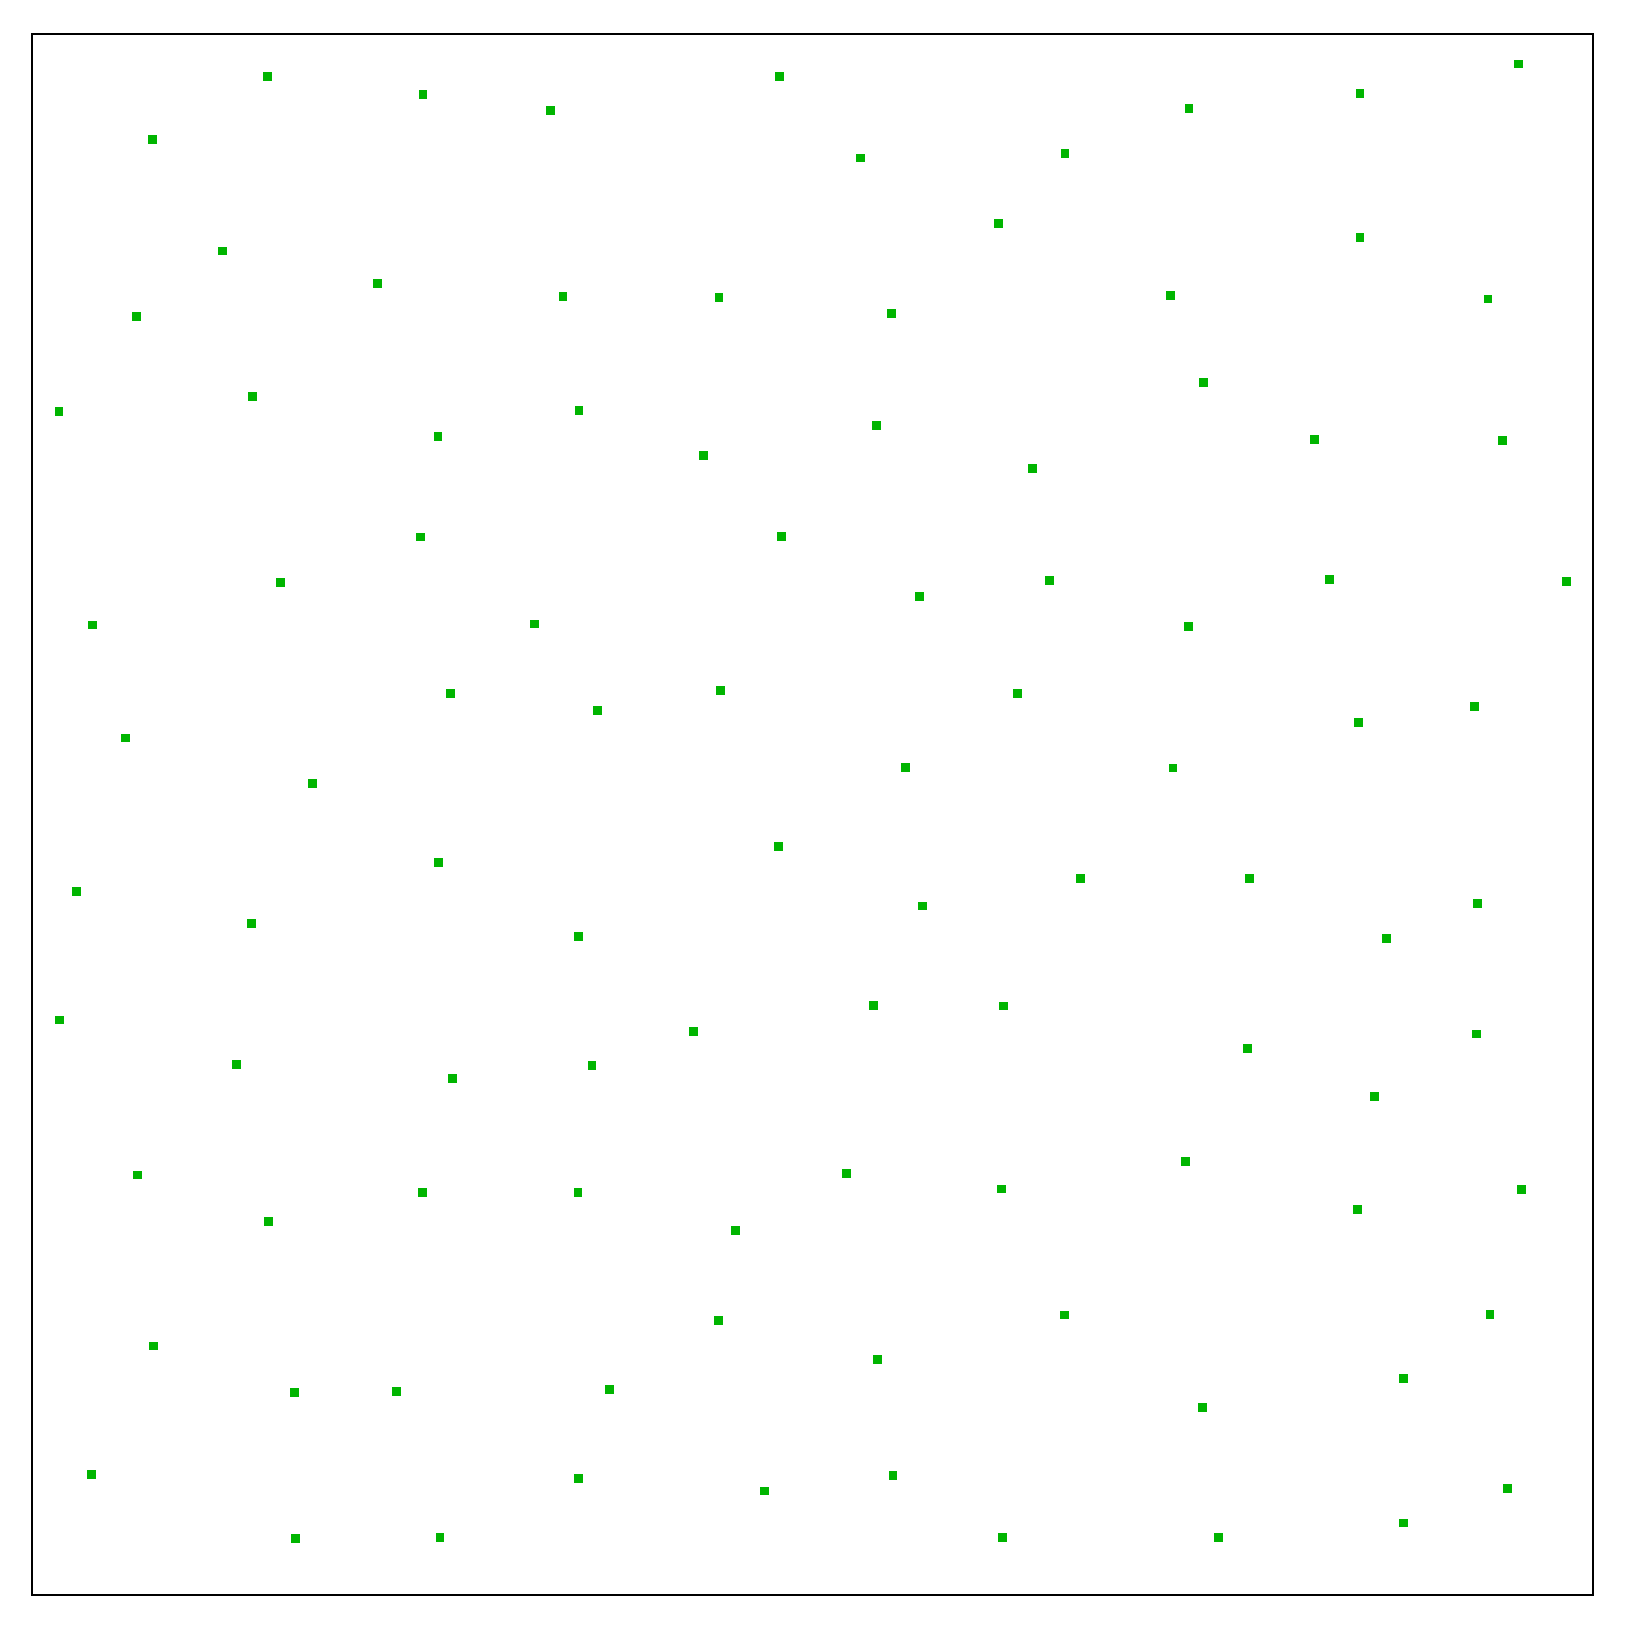
\includegraphics[width=0.33\textwidth]{img/createmap/nodes-start-grid-noise-3.eps}}
  \subfloat[Zcela n�hodn�]{\label{fig:createmap-random}\includegraphics[width=0.33\textwidth]{img/createmap/nodes-start-random.eps}}
  \caption{Po��te�n� rozlo�en� uzl�. Dal�� uk�zky jsou na p�ilo�en�m CD.}
  \label{fig:createmap}
\end{figure}




% STOPA VJEMU %%%%%%%%%%%%%%%%%%%%%%%%%%%%%%%%%%%%%%%%%%%%%%%%%%%%%%%%%%%%%%%%%%%%%%%%%%%%%%%%%%%%%%%%%%%%%%%%%%%%%%%%%%%%%%%%%%%%%%%%%%%


\subsection{Stopa vjemu}

Gravita�n� model se u�� z vjem� postupn�.
K tomu vyu��v� tzv. \emph{stopy vjemu}.
P�edstavuj� ur�itou m�ru pozornosti, kterou agent v�nuje jednomu p�edm�tu, kr�tkodob� ulo�en� vjem, kter� chv�li trv� a prostorovou mapu postupn� m�n�.
\\

\begin{definition}[Stopa vjemu]
Kdy� je v ur�it�m kroku simulace prostorov� map� p�ed�n vjem ke zpracov�n�, mapa si jej ulo�� a u�� se dle n�j nekolik dal��ch krok� simulace.
Takto ulo�en� vjem budeme naz�vat stopou vjemu.
Stopa vjemu je dvojice \emph{$<$pam�ov� stopa, intenzita$>$}, kde \emph{pam�ov� stopa}, je pam�ov� stopa p�edm�tu, kter� vjem vyvolal.
Intenzita stopy vjemu je p�i jej�m vytvo�en� odvozena z intenzity vjemu a v pr�b�hu �asu kles�.
Intenzita ur�uje m�ru, s jakou bude stopa vjemu ovliv�ovat prostorovou mapu.
\end{definition}

\begin{definition}[Vliv vjemu]
P�i vytvo�en� stopy vjemu je ur�ena jej� intenzita. Ta z�vis� na intenzit� p�vodn�ho vjemu a tzv. vlivu vjemu.
To je parametr modelu, kter� ovliv�uje rychlost u�en� prostorov� mapy. Budeme jej d�le zna�it $\eta_0$.
(EPCreateEnergy)
\end{definition}

Stopa vjemu postupn� sl�bne. Typicky b�hem n�kolika krok� simulace klesne jej� intenzita z po��te�n� hodnoty bl�zko k nule.
Jak dlouho stopa v map� z�stane, z�vis� na dvou parametrech: \emph{m��e sl�bnut�} a \emph{limitu zmizen�}.

\begin{definition}[M�ra slabnut�]
Parametr modelu \param{m�ra sl�bnut�} ur�uje rychlost kles�n� intenzity. Ovliv�uje, jak dlouho stopa vjemu existuje.
(EPFadeCoef)
\end{definition}

\begin{definition}[Limit zmizen�]
Parametr modelu \param{limit zmizen� } ur�uje, kdy stopa vjemu zmiz� z prostorov� mapy.
(EPFadeLimit)
\end{definition}

Zpracov�n� p��choz�ho vjemu je tedy pouze vytvo�en� stopy vjemu s odkazem na pam�ovou stopu.
Pokud v dan�m m�st� ji� stopa vjemu je, jej� intenzita je zv��ena. Po��te�n� intenzita stopy resp. zv��en� intenzity je d�no vzorcem:

\begin{equation} 
\eta(stopa) = \eta_0 \times \eta(vjem)
\label{formula:el-stopa-start-int}
\end{equation}


\begin{definition}[Dosah p�ita�livosti]
Parametr modelu \param{dosah p�ita�livosti} ur�uje, na jakou vzd�lenost jsou p�itahov�ny uzly mapy k stop�m vjemu. Vzd�len�j�� uzly nejsou p�itahov�ny.
(ELGravityRange)
\end{definition}

\begin{definition}[S�la p�ita�livosti]
Parametr modelu \param{s�la p�ita�livosti} ur�uje, jak velkou m�rou budou uzly prostorov� mapy p�itahov�ny ke stop� vjemu.
(ELGravityCoef)
\end{definition}

Jeden krok simulace stopy vjemu je pops�n v algoritmu \ref{alg:stopa-step}. V jeho prvn�m kroku je zkonstruov�na mno�ina okoln�ch uzl�:

\begin{equation} 
nodes_{around} = \{ n \in nodes ; dist(n, stopa) < dosah_{pritazlivost} \}
\label{formula:el-okolni-uzly-g}
\end{equation}


\begin{algorithm}[h!]
\caption{Jeden krok simulace pro stopu vjemu}
\label{alg:stopa-step}
\begin{algorithmic}[1]
\State $nodes_{around} \gets$ v�echny uzly v okol� stopy dle $dosah_{pritazlivost}$
\ForAll{$node \in nodes_{around}$}
	\State $node_{xy} \gets node_{xy} + \Delta_{xy}$ dle vzorce \eqref{formula:el-ep-gravitace} \label{alg:step-step-gravitace}
\EndFor
\ForAll{$node \in nodes_{around}$}
	\State $\Delta \eta \gets \eta(node, bod)$ dle vzorce \eqref{formula:el-intenzita} \label{alg:step-step-intenzita}
	\State zv��en� intenzity vazby $node$ - pam�ov� stopa p�edm�tu\footnote{Nejedn� se o stopu vjemu ale o pam�ovou stopu p�edm�tu definovanou v kapiotle \ref{chapter-pamet-predmety}} o $\Delta \eta$
\EndFor
\State $\eta(stopa) \gets \eta(stopa) \times fade_{\eta}$
\If{$\eta(stopa) < \eta_{forget}$}
	\State zmizen� stopy vjemu
\EndIf
\end{algorithmic}
\end{algorithm}

Na ��dku \ref{alg:step-step-gravitace} je pou�ita zm�na polohy uzlu $\Delta_{xy}$, je d�na vzorcem:

\begin{equation} 
\Delta_{xy}(node, stopa) = \frac{\eta(stopa)}{\eta_0} \times \frac{ sila_{pritazlivost} }{ dist(node, stopa)^2 \times \mu(node) }
\label{formula:el-ep-gravitace}
\end{equation}
\\

Na ��dku \ref{alg:step-step-intenzita} je zv��ena intenzita vazby mezi uzlem a pam�ovou stopu.
Zv��en� je d�no podobn�m vzorcem jako \eqref{formula:intenzita-vazby} s jedin�m rozd�lem, �e m�sto vjemu se pracuje s jeho stopou:

\begin{equation} 
\Delta \eta(node, stopa) = \eta(stopa) \times \frac{ norm( dist(node, stopa) ) }
{\sum_{n \in nodes_{around}}
  norm( dist(n, stopa) )
}
\label{formula:el-intenzita}
\end{equation}
\\

kde $nodes_{around}$ je mno�ina v�ech uzl� v okol� stopy vjemu.
Funkce $norm$ je libovoln� klesaj�c� funkce maj�c� obor hodnot $<0,1>$, nap�. nep��m� �m�ra $norm(x) = 1/max(1,x)$ �i Gaussova funkce.
\\


Na konci algoritmu jsou pou�ity dva parametry modelu: \param{limit zmizen�} $\eta_{forget}$ a \param{m�ra slabnut�} $fade_{\eta}$.
\\


% ODPUDIVOST UZLU %%%%%%%%%%%%%%%%%%%%%%%%%%%%%%%%%%%%%%%%%%%%%%%%%%%%%%%%%%%%%%%%%%%%%%%%%%%%%%%%%%%%%%%%%%%%%%%%%%%%%%%%%%%%%%%%%%%%%%%%%%%

\subsection{Odpudivost uzl�}

V ka�d�m kroku simulace se uzly, kter� jsou p��li� bl�zko u sebe, odpuzuj�.

\begin{definition}[Dosah odpudivosti]
Parametr modelu dosah odpudivosti ur�uje, na jakou vzd�lenost se uzly mapy je�t� odpuzuj�. Vzd�len�j�� uzly se neodpuzuj�.
(ELAntigravityRange)
\end{definition}

\begin{definition}[S�la odpudivosti]
Parametr modelu \param{s�la odudivosti} ur�uje, jak moc se uzly mapy odpuzuj�. P�sob� jako opak s�ly p�ita�livosti.
(ELAntigravityRange)
\end{definition}

\begin{definition}[Vliv napln�nosti]
Parametr modelu \param{vliv napln�nosti} ur�uje, jak velk� vliv m� napln�nost uzlu na jeho odpudivost s ostatn�mi uzly.
(ELAGUsageCoef)
\end{definition}

\begin{definition}[Limit pohybu uzlu]
Parametr modelu \param{limit pohybu} ur�uje maxim�ln� mo�nou zm�nu polohy uzlu v jednom kroku simulace.
(MaxELNodeMove)
\end{definition}

Zm�na polohy uzlu kv�li odpudivosti je sou�et odpudiv�ch sil okoln�ch uzl� a je nep��mo �m�rn� napln�nosti uzlu.
Nejd��ve jsou ur�eny okoln� uzly jako mno�ina:

\begin{equation} 
nodes_{around} = \{ n \in nodes ; dist(n, stopa) < dosah_{odpudivost} \}
\label{formula:el-okolni-uzly-ag}
\end{equation}


Pro v�echny okoln� uzly je spo�tena vz�jemn� odpudivost dle vzorce:

\begin{equation} 
odpudivost(n_i, n_j) = \frac{ sila_{odpudivost} }{ dist'(n_i, n_j)^2 \times \mu'(n_i) \times \mu'(n_j) } 
\label{formula:el-odpudivost}
\end{equation}

kde

\begin{equation} 
dist'(a,b) = max(1,dist(a,b))
\end{equation}

a

\begin{equation} 
\mu'(node) = max(\mu_{vliv},\mu'(node))
\end{equation}
 
Funkce $max$ jsou pou�ity, aby zabr�nili d�len� nulou a sn�ili vliv velmi mal� vzd�lenosti mezi dv�ma uzly a velmi mal� napln�nosti na odpudivost uzl�.
V�sledky s r�zn�mi hodnotami \param{vlivu napln�nosti} jsou v kapitole \ref{chapter-test-ag}.
\\

Po ur�en� v�ech odpudiv�ch sil, kter� na uzly p�sob�, jsou polohy uzl� upraveny dle t�chto sil a jejich aktu�ln� napln�nosti:

\begin{equation} 
\Delta_{xy}(node) = \frac{
\sum_{\substack{
   n \in nodes
  }}
  odpudivost(n, node)
}{ max(1, \mu(node)) } 
\label{formula:el-odpudivost}
\end{equation}
\\

Funkce $max$ je ve vzorci op�t pou�ita, aby zabr�nila d�len� nulou a p��li� velk�m zm�n�m polohy uzl� pro $\mu(node) \to 0$.
P�esto je mo�n�, �e se v jednom kroku simulace nas��taj� takov� odpudiv� a p�ita�liv� s�ly, �e by zm�na polohy uzlu mohla p�es�hnout rozumnou mez.
Nechceme, aby kv�li kr�tkodob�m stav�m s�t� \footnote{nap�. p�i vytvo�en� nov�ho uzlu prostorov� mapy} uzly p��li� m�nily svou polohu.
\\

P�idali jsme tedy omezen� na maxim�ln� mo�n� pohyb uzlu - parametr modelu \param{limit pohybu}.
Pokud by se poloha uzlu m�la zm�nit v jednom kroku simulace o v�ce ne� tento limit, zm�n� se pouze o tento limit.
Alternativn� �e�en� by bylo zmen�it parametr \param{s�la odpudivosti} a \param{s�la p�ita�livosti} a prov�st v�ce krok� simulace.
To je v�ak velmi n�ro�n� na v�kon a v��e uveden� �e�en� toto vlastn� imituje.
\\



\subsection{Omezen� pohybu uzl�}
N�sledkem odpudivosti uzl� je mo�n�, �e se model bude sna�it p�esunout uzel mimo sv�t, resp. vn� polygonu sv�t reprezentuj�c�.
V tom p��pad� je uzel na okraj sv�ta, tj. na hranu polygonu v m�st� jej�ho pr�se��ku s �se�kou p�edstavuj�c� pl�novanou trajektori� uzlu.
Pokud se v dal��ch kroc�ch simulace bude model op�t sna�it p�esunout uzel vn� polygonu, bude jeho trajektorie prom�tnuta na hranu polygonu, na kter� uzel le��.
Uzel tak bude "klouzat" po hran� polygonu, jak je uk�z�no na obr�zku \ref{fig:slide-on-edge}.
\\

\begin{figure}[h]
  \centering
  \scalebox{0.8}{\includegraphics{img/slide-on-edge.ps}}
  \caption{Zm�na posunu uzlu, kdy� naraz� na hranu polygonu}
  \label{fig:slide-on-edge}
\end{figure}





% ZMENA POCTU UZLU %%%%%%%%%%%%%%%%%%%%%%%%%%%%%%%%%%%%%%%%%%%%%%%%%%%%%%%%%%%%%%%%%%%%%%%%%%%%%%%%%%%%%%%%%%%%%%%%%%%%%%%%%%%%%%%%%%%%%%%%%%%

\subsection{Vytv��en� uzl�}

Je ��douc�, aby se po�et uzl� prostorov� mapy v pr�b�hu simulace m�nil, dle po�tu p�edm�t�, kter� agent vid�l resp. dle �etnosti a intenzity vjem�.
Mapa tedy vytv��� nov� uzly a zapom�n� existuj�c� uzly. 
Nov� uzly vytv��� stopy vjemu na z�klad� jejich intenzity.
Zapom�n�n� uzl� se d�je v ka�d�m kroku simulace resp. v ka�d�m kroku simulace je ur�it� pravd�podobnost, �e dojde k zapomenut� uzlu.
\\

\begin{definition}[Cena vytvo�en� uzlu]
Vytvo�en� nov�ho uzlu stoj� ur�it� mno�stv� intenzity stopy vjemu. Toto mno�stv� budeme naz�vat cena vytvo�en� uzlu a d�le jej budeme zna�it $cost_{create}$.
\end{definition}

\begin{definition}[Odchylka vytvo�en� uzlu]
Parametr modelu \param{odchylka vytvo�en� uzlu} ur�uje, jak daleko od stopy vjemu m��e b�t nov� uzel vytvo�en.
Pokud bude roven nule, budou v�echny uzly vytv��eny p�esn� v poloze stopy vjemu. To by vedlo k d��ve uveden�m probl�m�m s vysokou odpudivost�.
(ELNodeAddNoise)
\end{definition}

\begin{definition}[Po��te�n� napln�nost uzlu]
Parametr modelu, ur�uj�c� po��te�n� napln�nost uzlu.
(MemObjIntenseToNewNode)
\end{definition}

Roz���ili jsme jeden krok simulace pro stopu vjemu - algoritmus \ref{alg:stopa-step} - o vytv��en� nov�ch uzl�, algoritmus \ref{alg:stopa-step-create}.

\begin{algorithm}[h!]
\caption{Vytv��en� uzl� v r�mci stopy vjemu}
\label{alg:stopa-step-create}
\begin{algorithmic}[1]
\State $p_{create} \gets$ pravd�podobnost vzniku nov�ho uzlu dan� vzorcem \eqref{formula:el-pst-node-create} \label{alg:ep-step-create}
\State $r \gets$ n�hodn� ��slo $r \in <0,1>$
\If{$r < p_{create}$}
  \State vytvo�en� nov�ho uzlu
  \State vytvo�en� vazby uzlu na pam�ovou stopu p�edm�tu
  \State $\eta(stopa) \gets \eta(stopa) - cost_{create}$ \label{alg:ep-step-cost}
\EndIf
\end{algorithmic}
\end{algorithm}


Na ��dku \ref{alg:ep-step-create} je pou�ita pravd�podobnost vytvo�en� nov�ho uzlu, ta je d�na vzorcem:
\begin{equation} 
p_{create}(\eta(stopa), cost_{create}) = \frac{\eta(stopa) - cost_{create}}{cost_{create}}
\label{formula:el-pst-node-create}
\end{equation}
\\

Nov� vytvo�en� uzel bude m�t stejnou polohu jako stopa vjemu s n�hodnou odchylkou \(\in <-\Delta,\Delta>\), kde $\Delta$ je \param{odchylka vytvo�en� uzlu}.
Jeho napln�nost bude \param{po��te�n� napln�nost uzlu}.
Bude vytvo�ena vazba mezi uzlem a pam�ovou stopou p�edm�tu, kter� je sou��st� stopu vjemu, kter� uzel vytvo�ila.
\\



\subsection{Zapom�n�n� uzl�}


\begin{definition}[Cena zapomenut� uzlu]
Zapomenut� uzlu stoj� ur�it� mno�stv� energii na zapom�n�n�. Toto mno�stv� budeme naz�vat cena zapomenut� uzlu a d�le jej budeme zna�it $cost_{forget}$.
\end{definition}

\begin{definition}[M�ra zapom�n�n� uzl�]
Parametr modelu \param{m�ra zapom�n�n� uzl�} ur�uje jak rychle bude prostorov� mapa zapom�nat uzly.
(ELForgetNodeRate)
\end{definition}

K zapomenut� m��e doj�t ka�d� kroku simulace. Vrstva uzl� akumuluje tzv. energii na zapom�n�n� $e_{forget}$.
Na za��tku je rovn� nule a v pr�b�hu simulace roste.
V ka�d�m kroku je zv��ena o hodnotu parametru \param{m�ra zapom�n�n� uzl�}.
D�le je ur�ena pravd�podobnost, �e bude zapomenut uzel $p_{forget}$:

\begin{equation} 
p_{forget} = \frac{e_{forget} - cost_{delete}}{cost_{forget}}
\label{formula:el-pst-forget}
\end{equation}

Pokud m� doj�t k zapomenut� uzlu, je vybr�n n�hodn� uzel a ten je odstran�n z prostorov� mapy v�etn� v�ech jeho vazeb na pam�ov� stopy.
Proces zapom�n�n� uzlu je pops�n algoritmem \ref{alg:node-forget}.

\begin{algorithm}[h!]
\caption{Zapom�n�n� uzl�}
\label{alg:node-forget}
\begin{algorithmic}[1]
\State $e_{forget} \gets e_{forget} + rate_{forget}$
\State $p_{forget} \gets$ pravd�podobnost zapomenut� uzlu dan� vzorcem \eqref{formula:el-pst-forget} \label{alg:el-forget}
\State $r \gets$ n�hodn� ��slo $r \in <0,1>$
\If{$r < p_{forget}$}
  \State $node \gets $ n�hodn� vybran� uzel
  \State $e_{forget} \gets e_{forget} - cost_{forget}$ \label{alg:el-forget-cost}
  \State zapomenut� uzlu
  \State lok�ln� simulace odpudivosti v okol� smazan�ho uzlu
\EndIf
\end{algorithmic}
\end{algorithm}

Kdy� je z mapy odstran�n uzel, m��e doj�t a typicky doch�z� k naru�en� nau�en�ho rovnom�rn�ho rozlo�en� uzl� v prostoru, smazan� uzel za sebou nech�v� pr�zdn� m�sto.
��st prostorov� mapy kolem smazan�ho uzlu by bylo vhodn� p�eu�it, p�em�stit uzly, aby byly op�t rovnom�rn� rozd�len�.
Proto je p�i smaz�n� uzlu provedeno n�kolik lok�ln�ch krok� simulace, kdy je prov�d�no pouze odpuzov�n� uzl� v okol� smazan�ho uzlu.
Tento proces m� dva parametry: \param{po�et opakov�n�} a \param{velikost okol�}.

\begin{definition}[Po�et opakov�n�]
Parametr modelu \param{po�et opakov�n�} ur�uje po�et opakov�n� lok�ln�ch krok� simulace.
(ELDeleteNodeReTrainCount)
\end{definition}

\begin{definition}[Velikost okol�]
Parametr modelu \param{velikost okol�} ur�uje velikost okol�, tj. uzly, jejich� poloha se m�n�.
(ELDeleteNodeReTrainRange)
\end{definition}



% CENA UZLU %%%%%%%%%%%%%%%%%%%%%%%%%%%%%%%%%%%%%%%%%%%%%%%%%%%%%%%%%%%%%%%%%%%%%%%%%%%%%%%%%%%%%%%%%%%%%%%%%%%%%%%%%%%%%%%%%%%%%%%%%%%


\subsection{Cena vytvo�en� a zapomenut� uzlu}

Cht�li bychom, aby po�et uzl� mapy se po ur�it� dob� ust�lil a aby tento po�et reflektoval �etnost vjem�.
V okam�iku, kdy agent m�stnost opust�, m�l by po�et uzl� mapy postupn� klesat.
Prostorov� mapa nebude dost�vat ��dn� vjemy a tedy ani vytv��et nov� uzly, bude je pouze zapom�nat.
Kles�n� po�etu uzl� by m�lo b�t pozvoln� a zpomalovat. Po�et uzl� by nem�l klesnout na nulu.

V��e uvedenou cenu vytvo�en� a zapomenut� uzlu m��eme ur�it mnoha zp�soby.
M��e b�t konstantn� �i m��e r�zn�mi zp�sby z�viset na aktu�ln�m po�tu uzl�.
V t�to kapitole uvedeme r�zn� mo�nosti, uk�eme v�sledky test� a vybereme nejlep�� �e�en�.
\\


\subsubsection{Konstantn� cena}

Nejjednodu��� mo�nost� je ur�it cenu jako konstantu. V pr�b�hu simulace se nebude m�nit.
Nem��e z�viset na �asu, proto�e po�et p�edm�t� ve sv�t� se m��e m�nit zcela n�hodn�, tedy ub�vat i p�ib�vat.
Nem��eme tedy ��ci, �e cena roste s dobou, kterou agent v m�stnosti str�vil.

\begin{figure}[h!]
  \centering
  \subfloat[EmptyRoom]{\label{fig:nc-100-empty}\includegraphics[width=0.5\textwidth]{img/nc/100-empty.eps}}
  \subfloat[FullRoom]{\label{fig:nc-100-full}\includegraphics[width=0.5\textwidth]{img/nc/100-full.eps}}
  \caption{Test konstantn� ceny}
  \label{fig:nc-fixed}
\end{figure}

V�sledek testu konstantn� ceny je na obr�zku \ref{fig:nc-fixed}. Graf zobrazuje po�et uzl� prostorov� mapy v �ase.
Na konkr�tn� hodnot� nez�le��, testy s jin�mi hodnotami ceny maj� obdobn� v�sledky obdobn�\footnote{Jsou na p�ilo�en�m CD}.
Pokud je cena konstantn�, v m�stnost s v�t��m po�tem p�edm�t� uzl� neust�le p�ib�v�.
V m�stnosti s mal�m po�tem p�edm�t� uzly miz� a jejich po�et kles� a� k nule.
Je tedy z�ejm�, �e cena nem��e b�t konstatn�.
\\


\subsubsection{Polynomi�ln� z�vislot na po�tu uzl�}

\begin{definition}[Cht�n� po�et uzl�]
Ze vzorce \eqref{formula:el-start-pocet-uzlu} je ur�en po��te�n� po�et uzl�.
Cht�n� po�et uzl� $n_{desired}$ je po�et uzl�, kter� by v prostoru m�ly b�t, ur�en� jen dle jeho velikosti.
Je to konstanta, dvojn�sobek po�tu uzl�, kter� jsou do prostoru um�st�ny na za��tku.
\end{definition}

Definujme cenu vytvo�en� uzlu $cost_{create}$ resp. zapomenut� uzlu $cost_{forget}$ jako funkci $n_{desired}$ a aktu�ln�ho po�tu uzl� $n_{c}$.
Pro jednoduchost budou tyto funkce symetrick� dle osy y, $cost_{create}$ bude rostouc� a $cost_{forget}$ klesaj�c�.
T�m zabr�n�me p��lis velk�m a rychl�m zm�n�m po�tu uzl�. Definujme funkce takto:
\\

\begin{equation} 
cost_{create}(n_{desired}, n_{c}) = \eta_0 \times \frac{n_{desired}}{n_{c}}
\label{formula:cost-create-linear}
\end{equation}

\begin{equation} 
cost_{forget}(n_{desired}, n_{c}) = \eta_0 \times \frac{n_{c}}{n_{desired}}
\label{formula:cost-forget-linear}
\end{equation}

kde $\eta_0$ je parametr modelu \param{vliv vjemu}.

V�sledky test� jsou na obr�zku \ref{fig:nc-linear-long}. Ukazuj�, �e takto definovan� ceny by fungovala pro dobu, kdy se agent pohybuje ve sv�t�.
V kroku 5000 opustil m�stnost a po�et uzl� b�hem 10000 resp. 15000 krok� klesl t�m�� na nulu.
\\

\begin{figure}[h!]
  \centering
  \subfloat[EmptyRoom]{\label{fig:nc-100-empty}\includegraphics[width=0.5\textwidth]{img/nc/linear-empty-long.eps}}
  \subfloat[FullRoom]{\label{fig:nc-100-full}\includegraphics[width=0.5\textwidth]{img/nc/linear-full-long.eps}}
  \caption{Test line�rn� ceny, agent opustil m�stnost v kroku 5000.}
  \label{fig:nc-linear-long}
\end{figure}


Je t�eba zabr�n�t klesnut� po�tu uzl� na nulu. Pokud zm�n�me cht�n� po�et uzl� $n_{desired}$, situaci nevy�e��me.
Definujme funkce jako kvadratick� takto:

\begin{equation} 
cost_{create}(n_{desired}, n_{c}) = \eta_0 \times (\frac{n_{desired}}{n_{c}})^2
\label{formula:cost-create-square}
\end{equation}

\begin{equation} 
cost_{forget}(n_{desired}, n_{c}) = \eta_0 \times (\frac{n_{c}}{n_{desired}})^2
\label{formula:cost-forget-square}
\end{equation}
\\

V�sledky test� jsou na obr�zku \ref{fig:cost-square-long}.
Kles�n� uzlu vlivem zapom�n�n� v dob�, kdy agent opustil m�stnost, spl�uje po�adavky,
alespo� pokud tato doba je pouze n�kolikan�sobek doby, kterou agent v m�stnosti str�vil.
V dob�, kdy agent byl v m�stnoti, po�et uzl� rostl, p�esto�e zobrazen� test byl proveden v m�stnosti obsahuj�c� pouze jedne p�edm�t.
To je zp�sobeno t�m, �e cena definovan� vzorcem \eqref{formula:cost-create-square} resp. \eqref{formula:cost-forget-square} p��li� m�n� po�et uzl� tak,
aby byl co nejv�ce roven cht�n�mu po�tu uzl� $n_{desired}$. Zvy�ov�n�m stupn� polynomu to jen urychl�.
\\

\begin{figure}[h!]
  \centering
  \includegraphics[width=1.0\textwidth]{img/nc/square-empty-long.eps}
  \caption{Test kvadratick� ceny v m�stnosti EmptyRoom, agent opustil m�stnost v kroku 5000.}
  \label{fig:cost-square-long}
\end{figure}



\subsubsection{Exponenci�ln� z�vislost na po�tu uzl�}
Definujme funkce takto:

\begin{equation} 
cost_{create}(n_{desired}, n_{c}) = coef_1 \times 3^{\displaystyle coef_2 \times \frac{ n_{c} - n_{desired} }{ n_{desired} } }
\label{formula:cost-create-exp}
\end{equation}

\begin{equation} 
cost_{forget}(n_{desired}, n_{c}) = coef_1 \times 3^{\displaystyle - coef_2 \times \frac{ n_{c} - n_{desired} }{ n_{desired} } }
\label{formula:cost-forget-exp}
\end{equation}
\\

Hodnotu koeficient $coef_1$ jsme ur�ili pevn�, je rovna hodnot� parametr \param{vliv vjemu} $\eta_0$.
Provedli jsme testy r�zn�ch hodnot koeficientu $coef_2$, v�sledky jsou na obr�zc�ch \ref{fig:nc-exp-20}, \ref{fig:nc-exp-50}, \ref{fig:nc-exp-100} a \ref{fig:nc-exp-200}.
Vypl�v� z n�ch, �e $coef_2$ ur�uje m�ru, s jakou se po�et uzl� bude bl�it cht�n�mu po�tu uzl� $n_{desired}$.
Po dosa�en� rovnov�n�ho po�tu uzl�, ur�uje $coef_2$ velikost odchylky, jak moc bude po�et uzl� fluktuovat.
��m je $coef_2$ vy���, t�m rychleji se po�e uzl� bl�� $n_{desired}$ a t�m men�� je odchylka.
Nejlep�� se jev� hodnota $coef_2 = 1$.
\\

\begin{figure}[p]
  \centering
  \subfloat[EmptyRoom]{\label{fig:nc-exp-20-empty}\includegraphics[width=0.5\textwidth]{img/nc/exp-20-empty.eps}}
  \subfloat[FullRoom]{\label{fig:nc-exp-20-full}\includegraphics[width=0.5\textwidth]{img/nc/exp-20-full.eps}}
  \caption{Test exponenci�ln� ceny pro $coef_2 = \frac{2}{5}$.}
  \label{fig:nc-exp-20}
\end{figure}

\begin{figure}[p]
  \centering
  \subfloat[EmptyRoom]{\label{fig:nc-exp-50-empty}\includegraphics[width=0.5\textwidth]{img/nc/exp-50-empty.eps}}
  \subfloat[FullRoom]{\label{fig:nc-exp-50-full}\includegraphics[width=0.5\textwidth]{img/nc/exp-50-full.eps}}
  \caption{Test exponenci�ln� ceny pro $coef_2 = 1$.}
  \label{fig:nc-exp-50}
\end{figure}

\begin{figure}[p]
  \centering
  \subfloat[EmptyRoom]{\label{fig:nc-exp-100-empty}\includegraphics[width=0.5\textwidth]{img/nc/exp-100-empty.eps}}
  \subfloat[FullRoom]{\label{fig:nc-exp-100-full}\includegraphics[width=0.5\textwidth]{img/nc/exp-100-full.eps}}
  \caption{Test exponenci�ln� ceny pro $coef_2 = 2$.}
  \label{fig:nc-exp-100}
\end{figure}

\begin{figure}[p]
  \centering
  \subfloat[EmptyRoom]{\label{fig:nc-exp-200-empty}\includegraphics[width=0.5\textwidth]{img/nc/exp-200-empty.eps}}
  \subfloat[FullRoom]{\label{fig:nc-exp-200-full}\includegraphics[width=0.5\textwidth]{img/nc/exp-200-full.eps}}
  \caption{Test exponenci�ln� ceny pro $coef_2 = 4$.}
  \label{fig:nc-exp-200}
\end{figure}

Provedli jsme je�t� test zapom�n�n�, tedy s dlouho dobou, kdy je agent mimo m�stnost. Jeho v�sledky jsou na obr�zku \ref{fig:nc-exp-50-long}.
Ukazuj�, �e takto definovan� ceny si se zapom�n�n�m nedok�� v�bec poradit, po�et uzl� kles� p��li� rychle a brzy dos�hne hodnoty nula.
\\

\begin{figure}[h!]
  \centering
  \subfloat[EmptyRoom]{\label{fig:nc-exp-50-empty-long}\includegraphics[width=0.5\textwidth]{img/nc/exp-50-empty-long.eps}}
  \subfloat[FullRoom]{\label{fig:nc-exp-50-full-long}\includegraphics[width=0.5\textwidth]{img/nc/exp-50-full-long.eps}}
  \caption{Test exponenci�ln� ceny pro $coef_2 = 1$ v�etn� zapom�n�n�, agent opustil m�stnost v kroce 5000.}
  \label{fig:nc-exp-50-long}
\end{figure}

Jako �e�en� jsme zvolili sou�et dvou exponenci�ln�ch funkc� \eqref{formula:cost-create-exp} s r�zn�mi hodnotami $coef_1$ a $coef_2$.
Ozna�me zobecn�n� funkce \eqref{formula:cost-create-exp} takto:

\begin{equation} 
cost^{coef_1}_{coef_2}(n_{desired}, n_{c}) = coef_1 \times 3^{\displaystyle coef_2 \times \frac{ n_{c} - n_{desired} }{ n_{desired} } }
\label{formula:cost-coefs}
\end{equation}
\\

Pak definujme cenu vytvo�en� a zapomenut� uzlu takto:

\begin{equation} 
cost_{create}(n_{desired}, n_{c}) = cost^{\eta_0}_{1}(n_{desired}, n_{c}) + cost^{\frac{1}{10000}}_{22}(n_{desired}, n_{c})
\label{formula:cost-create-sum}
\end{equation}

\begin{equation} 
cost_{forget}(n_{desired}, n_{c}) = cost^{\eta_0}_{1}(n_{desired}, n_{c}) + cost^{\frac{1}{10000}}_{-22}(n_{desired}, n_{c})
\label{formula:cost-forget-sum}
\end{equation}
\\

V�sledky testu pro takto definovanou cenu jsou na obr�zku \ref{fig:nc-expsum-50}.
\\

\begin{figure}[h!]
  \centering
  \subfloat[EmptyRoom]{\label{fig:nc-expsum-50-empty-long}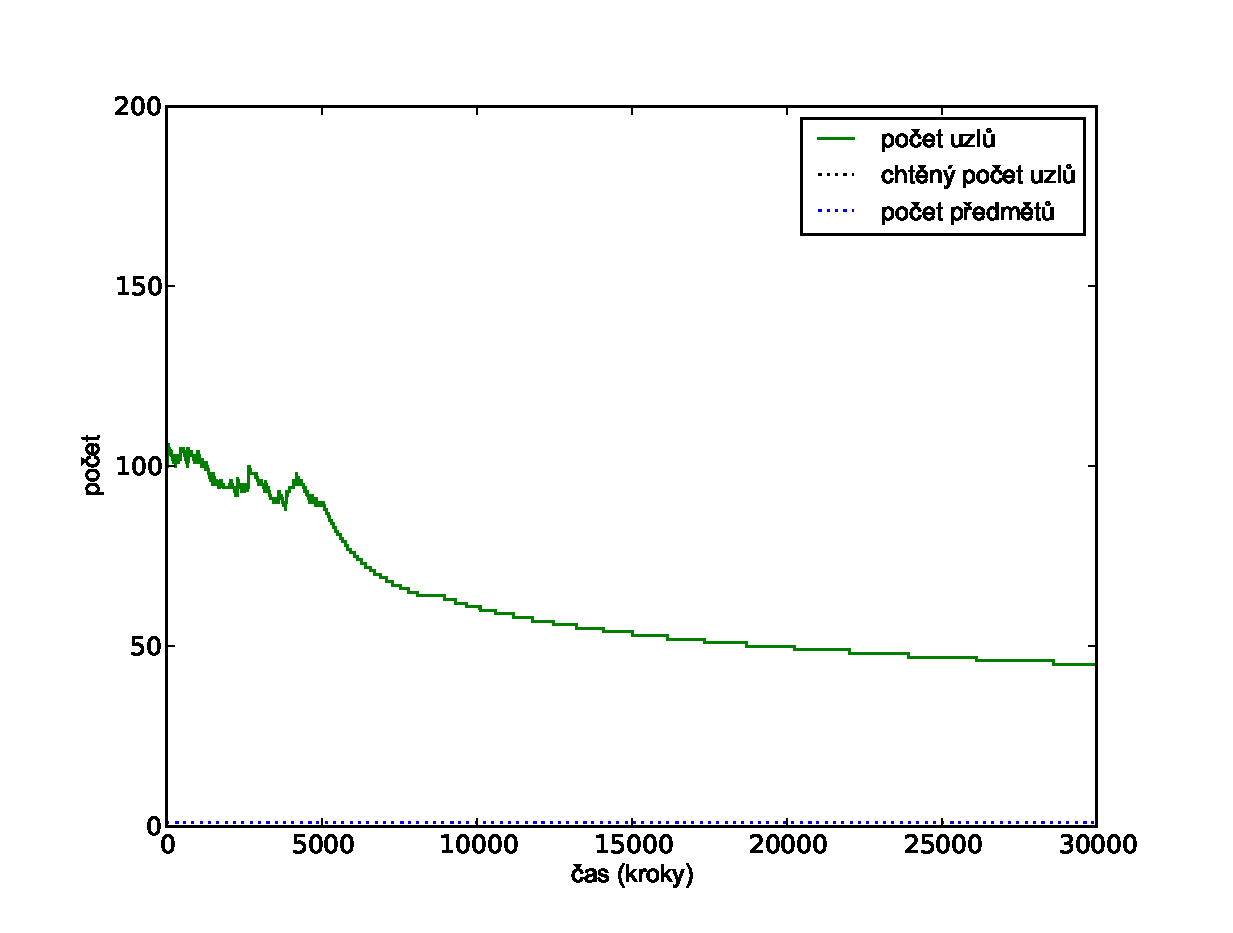
\includegraphics[width=0.5\textwidth]{img/nc/expsum-50-empty.eps}}
  \subfloat[FullRoom]{\label{fig:nc-expsum-50-full-long}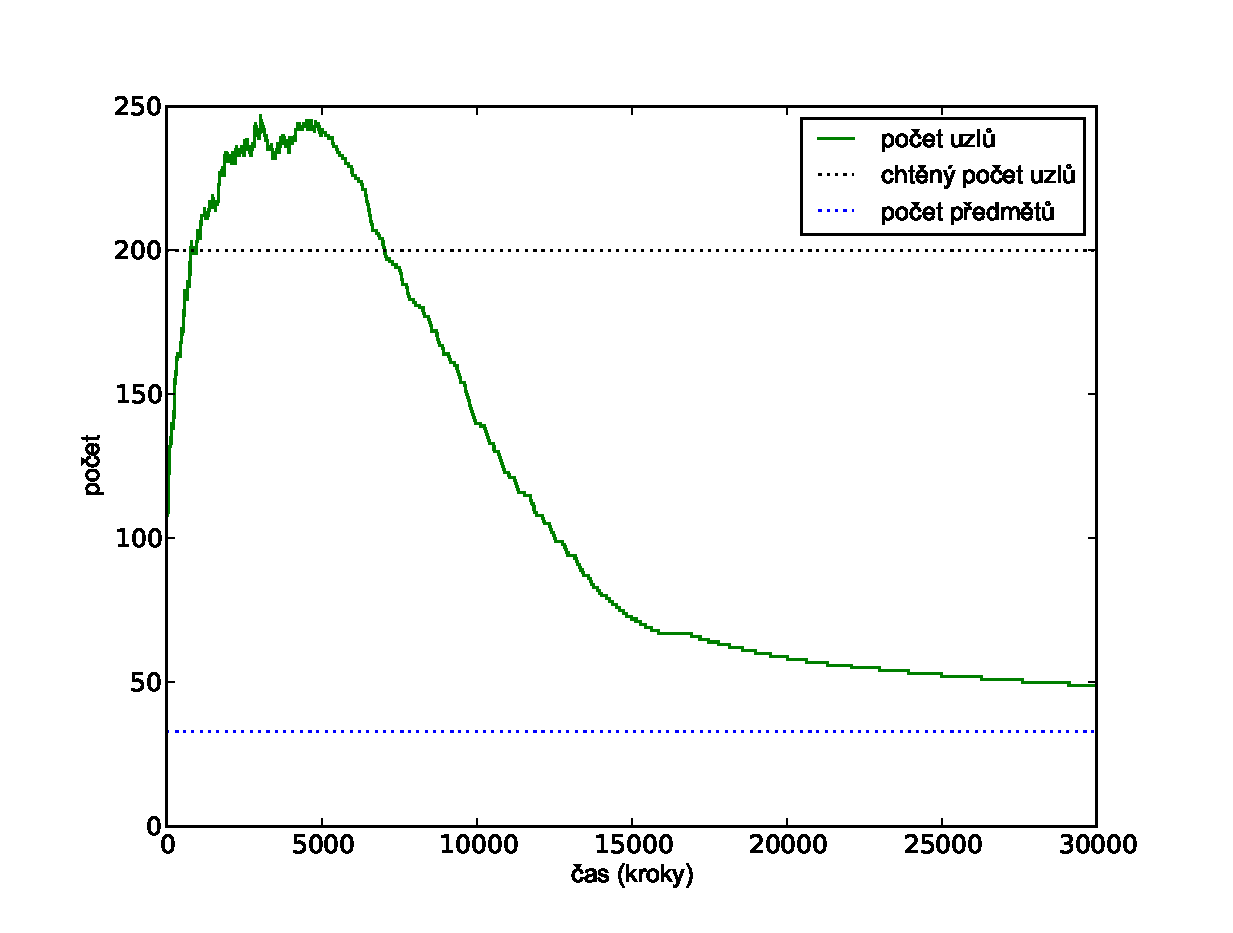
\includegraphics[width=0.5\textwidth]{img/nc/expsum-50-full.eps}}
  \caption{Test ceny jako sou�tu exponenciel, agent opustil m�stnost v kroce 5000.}
  \label{fig:nc-expsum-50}
\end{figure}


?? ToDo: OBR grafy scitanych exponenciel ??
\\


% HIEARCHIE %%%%%%%%%%%%%%%%%%%%%%%%%%%%%%%%%%%%%%%%%%%%%%%%%%%%%%%%%%%%%%%%%%%%%%%%%%%%%%%%%%%%%%%%%%%%%%%%%%%%%%%%%%%%%%%%%%%%%%%%%%%


\subsection{Hiearchie}
Jedn�m z po�adavk� na model vrstvy uzl� je, aby um�l vytv��et hiearchii uzl�. Model mus� b�t schopen rozpoznat m�sta s vy��� hustotou uzl�.
\\
Mno�stv� odpudivosti v uzlu je sledov�no a kdy� p�ekro�� limit dan� modelem, parametr HLAGNeeded, algoritmus \ref{alg:hl-create} vytvo�� nov� uzel vy��� �rovn�.
?? ToDo? ??
\\


% MISTA - PLACES %%%%%%%%%%%%%%%%%%%%%%%%%%%%%%%%%%%%%%%%%%%%%%%%%%%%%%%%%%%%%%%%%%%%%%%%%%%%%%%%%%%%%%%%%%%%%%%%%%%%%%%%%%%%%%%%%%%%%%%%%%%

\subsection{Vytv��en� m�st} \label{chapter-place-detect}


\begin{definition}[Mno�stv� odpudivosti]
Uzl�m prostorov� mapy p�id�me dal�� vlastnost \emph{mno�stv� odpudivosti}, kter� vyjad�uje hustotu uzl� v jeho okol�.
Budeme jej zna�it $\varrho(node)$.
Nejedn� se pouze o aktu�ln� stav, tato vlastnost m� ur�itou pam�, odr�� stav v psledn�ch n�kolika des�tk�ch a� stovk�ch krok� simulace.
Jak p�esn� se bude mno�stv� odpudivosti uzlu m�nit, z�vis� na dvou parametrch modelu:
\param{rychlost r�stu} a \param{rychlost kles�n�}.
\end{definition}

\begin{definition}[Rychlost r�stu]
Parametr modelu \param{rychlost r�stu $\varrho(node)$} ur�uje, jak rychle bude r�st mno�stv� odpudivosti.
Budeme jej zna�it $\Delta^{+}_{\varrho}$.
(ELAGAddCoef)
\end{definition}

\begin{definition}[Rychlost kles�n�]
Parametr modelu \param{rychlost kles�n� $\varrho(node)$} ur�uje, jak rychle bude klesat mno�stv� odpudivosti.
Budeme jej zna�it $\Delta^{-}_{\varrho}$.
(ELAGFadeOut)
\end{definition}

P�i vytvo�en� uzlu je mno�stv� odpudivosti rovno nule. V ka�d�m kroku, p�i po��t�n� odpudiv�ch sil p�sob�c�ch na uzel, je zv��eno o:

\begin{equation} 
\Delta_{\varrho}(node) = \sum_{
 	\substack{
		n \in nodes
	}}
  |odpudivost(n, node)| \times \Delta^{+}_{\varrho}
\label{formula:el-agamount}
\end{equation}
\\

kde $nodes$ je mno�ina okoln�ch uzl� z�sk�na dle \eqref{formula:el-okolni-uzly-ag}.
Mno�stv� odpudivosti uzlu v kroku $i+1$ je d�no vzorcem:

\begin{equation} 
\varrho_{i+1}(node) = \varrho_{i}(node) + \Delta_{\varrho}(node) - \Delta^{-}_{\varrho}
\label{formula:el-agamount-delta}
\end{equation}
\\

V pr�b�hu simulace se m�n� hustota uzl� v r�zn�ch ��stech sv�ta.
Cht�li bychom, aby agent rozpoznal ��sti sv�ta, kde je hustota uzl�\footnote{Vy��� hustota uzl� je zp�sobena p��tomnost� v�ce p�edm�t�} v�t�� a 
vytvo�il si tak p�edstavu konkr�tn�ch m�st ve sv�t�.
\\

\begin{definition}[M�sto]
M�sto je kruh dan� polohou st�edu a polom�rem. Model vytv��� hiearchii m�st, m�sta postupn� d�l� na men��, tak�e m�sto obsahuje dal�� \emph{podm�sta},
n�le�en� podm�sta do m�sta budeme zna�it $podmisto \in misto$.
\end{definition}

\begin{definition}[�rov�� m�sta]
M�sto m� svou �rov��, kter� ur�uje, jak je hluboko v hiearchii m�st resp. podm�st. �rove� m�sta je o jedna vet��, ne� �rove� nad�azen�ho m�sta.
\end{definition}

Na za��tku simulace je vytvo�eno jedno m�sto, kter� pokr�v� cel� sv�t.
V�echny uzly prvotn� mapy n�le�� tomuto prvn�mu m�stu. Jeho poloha a polom�r se nem�n�. 
V pr�b�hu simulace je toto m�sto d�l�no na podm�sta a uzly budou n�le�et do v�ce m�st.
Uzel n�le�� m�stu pokud do n�j geometricky pat��:

\begin{equation} 
node \in misto \iff dist(node,misto) < polomer(misto)
\label{formula:el-node-in-misto-geo}
\end{equation}


\begin{definition}[Mno�stv� odpudivosti m�sta]
M�sto m� sv� mno�stv� odpudivosti $\varrho(misto)$ rovn� sou�tu mno�stv� odpudivosti jeho uzl�:
\begin{equation} 
\varrho(misto) = \sum_{n \in misto} \varrho(node,misto)
\label{formula:el-agamount-mista-geo}
\end{equation}
kde funkce $\varrho(node,misto)$ ur�uje, jakou ��st mno�stv� odpudivosti uzlu $\varrho(node)$ p��slu�� dan�mu m�stu.
Pokud by ka�d� m�sto dostalo v�echno $\varrho(node)$, do�lo by k neust�l�mu vytv��en� dal��ch podm�st.
\end{definition}

\begin{definition}[Intenzita m�sta]
M�sto m� svou intenzitu, jedn� se o analogii k intenzit� stopy vjemu resp. k napln�nosti uzlu. Intenzita m�sta m� vliv na zm�nu jeho polom�ru a polohy m�sta.
Lze ji ch�pat jako $\varrho(misto)$ s pam�t�.
\end{definition}

\begin{definition}[Rychlost r�stu intenzity]
Parametr modelu \param{rychlost r�stu intenzity} $\Delta^{+}_{\eta}$ ur�uje, jak rychle poroste intenzita m�sta v z�vislosti na jeho aktu�ln� intenzit�.
\end{definition}

\begin{definition}[Limit vzniku podm�sta]
Parametr modelu \param{limit vzniku podm�sta} ur�uje mno�stv� odpudivosti m�sta nutn� pro vytvo�en� dal��ho podm�sta.
(PlacesAGNeeded)
\end{definition}

\begin{definition}[Limit zapomenut� m�sta]
Parametr modelu \param{limit zapomenut� m�sta} ur�uje, kdy bude m�sto zapomenuto. Pokud bude intenzita m�sta men�� ne� tento limit, agent m�sto zapomene.
(PlacesAGMin)
\end{definition}

\begin{definition}[Rychlost kles�n� intenzity]
Parametr modelu \param{rychlost kles�n� intenzity} m�sta ur�uje, jak rychle bude agent m�sta zapom�nat.
(PlaceAGFadeOut)
\end{definition}

\begin{definition}[Pohyblivost m�st]
Parametr modelu \param{pohyblivost m�st} ur�uje rychlost pohybu m�st, jak moc se bude m�nit jejich poloha.
(PlaceMoveCoef)
\end{definition}

\begin{algorithm}[h!]
\caption{Jeden krok simulace m�sta}
\label{alg:el-step-misto}
\begin{algorithmic}[1]
\State $\varrho(misto) \gets $ mno�stv� odpudivosti dle vzorce \eqref{formula:el-agamount-mista-geo} \label{alg:el-step-misto-varrho}
\State $\eta(misto) \gets \eta(misto) + \Delta_{\eta(misto)}$ dle vzorce \eqref{formula:el-mist-delta-eta} \label{alg:el-step-misto-eta}
\If{$\eta(misto) < \eta_{forget} \times (uroven(misto)-1)$}
  \State zapomenut� m�sta
\EndIf
\If{$\varrho(misto) > \varrho_{split} \times 2^{uroven(misto)-1} $}
  \State vytvo�en� podm�st \label{alg:el-step-misto-podmista}
\EndIf
\State ur�en� v�en�ho centroidu m�sta $c_w$ \label{alg:el-step-misto-centroid}
\State ur�en� nov� polohy m�sta \label{alg:el-step-misto-misto}
\State ur�en� polom�ru m�sta dle jeho $\eta(misto)$ dle vzorce \eqref{formula:el-misto-range} \label{alg:el-step-misto-polomer}
\end{algorithmic}
\end{algorithm}

Ka�d� krok simulace je pro ka�d� m�sto proveden proces popsan� v algoritmu \ref{alg:el-step-misto}.
V algoritmu jsou pou�ity parametry modelu \param{limit vzniku podm�sta} $\varrho_{split}$ a \param{limit zapomenut� m�sta} $\eta_{forget}$.
Na ��dku \ref{alg:el-step-misto-eta} je zm�n�na intenzita m�sta o $\Delta_{\eta(misto)}$, to je ur�en� vzorcem:

\begin{equation} 
\Delta_{\eta(misto)} = \varrho_{total}(misto) \times \frac{1}{ max(1, \eta(misto) \times \Delta^{+}_{\eta}) } - fade_{\eta}
\label{formula:el-mist-delta-eta}
\end{equation}

kde $\Delta^{+}_{\eta}$ je parametr modelu \param{rychlost r�stu intenzity m�sta},
$fade_{\eta}$ je parametr modelu \param{rychlost kles�n� intenzity} a $\varrho_{total}(misto)$ je celkov� mno�stv� odpudivosti:
\begin{equation} 
\varrho(misto) = \sum_{n \in misto} \varrho(node) + \sum_{m \in misto} \varrho(m)
\label{formula:el-agamount-mista}
\end{equation}
\\

Na ��dku \ref{alg:el-step-misto-centroid} je ur�en v�en� centroid m�sta:
\begin{equation} 
c_w(misto) = \frac{\displaystyle \sum_{n \in misto} n_{xy} \times \varrho(n) + \sum_{m \in misto} m_{xy} \times \varrho_{total}(m) }{\displaystyle \varrho_{total}(misto)}
\label{formula:el-centroid-mista}
\end{equation}

kde $n$ je uzel a $m$ podm�sto.
Pak je poloha m�sta je pot� posunuta sm�rem k centroidu o $\Delta_{xy}$ ur�en� vzorcem:
\begin{equation} 
\Delta_{xy} = dist(misto,centorid) \times min \left(1,\frac{\eta_0(misto)}{\eta(misto)}\right) \times pohyblivost_{mist}
\label{formula:el-agamount-mista}
\end{equation}

kde $pohyblivost_{mist}$ je parametr modelu \param{pohyblivost m�st}.
Na ��dku \ref{alg:el-step-misto-polomer} je ur�en nov� polom�r m�sta dle vzorce:

\begin{equation} 
polomer(misto) = polomer_0(misto) \times \left( \frac{2}{5} \times \frac{\eta_0(misto)}{\eta(misto)} + \frac{3}{5} \right)
\label{formula:el-misto-range}
\end{equation}

kde $\eta_0(misto)$ je po��te�n� intenzita m�sta a $polomer_0(misto)$ je po��te�n� polom�r m�sta, tedy jeho polom�r a intenzita, kdy� bylo vytvo�eno.
Hodnoty $\frac{2}{5}$ a $\frac{3}{5}$ ur�uj�, jak moc se polom�r m�sta m��e zm�nit.
\\

Pokud v algoritmu na ��dce \label{alg:el-step-misto-podmista} dojde k d�len� m�sta resp. vytv��en� podm�st, je proveden n�sleduj�c� proces.
\\

\begin{algorithm}[h!]
\caption{Rozd�len� m�sta na podm�sta}
\label{alg:el-misto-split}
\begin{algorithmic}[1]
\State $node \gets \arg \max_{n \in misto} \varrho(n) $ 
\State vytvo�en� nov�ho podm�sta
\State $podmisto_{xy} = node_{xy}$
\State $polomer(podmisto) = polomer(misto) / 2$
\State ur�en� uzl� podm�sta, $podmisto_{nodes} \subseteq misto_{nodes}$
\State $\varrho(podmisto) \gets $ mno�stv� odpudivosti dle vzorce \eqref{formula:el-agamount-mista}
\State $\eta(podmisto) \gets \varrho(podmisto)$
\State ur�en� v�en�ho centroidu m�sta $c_w$
\State ur�en� nov� polohy m�sta \label{alg:el-step-misto-misto}
\State ur�en� polom�ru m�sta dle jeho $\eta(misto)$ dle vzorce \eqref{formula:el-misto-range}
\end{algorithmic}
\end{algorithm}

Nejd��ve je vybr�n uzel s nejv�t��m mno�stv�m odpudivosti, s n�m je proveden algoritmus \ref{alg:el-misto-split}.
Pak je znovu spo�teno mno�stv� odpudivosti $\varrho(misto)$ m�sta a pokud nekleslo pod polovinu, je algoritmus \ref{alg:el-misto-split} zopakov�n.
Algoritmus \ref{alg:el-misto-split} je prov�d�n tak dlouho, ne� $\varrho(misto)$ klesne pod polovinu p�vodn� hodnoty.
Pokud nov� vytvo�en� podm�sto m� men�� mno�stv� odpudivosti ne� parametr \param{limit zapomenut� m�sta}, je ihned zru�eno a m�sto nen� d�le d�leno.
\\

Po proveden� algoritmu \ref{alg:el-step-misto} pro v�echna m�sta prostorov� mapy, je aktualizov�na p��slu�nost uzl� do m�st dle \eqref{formula:el-agamount-mista-geo}.
\\


Ot�zkou z�st�v� funkce $\varrho(node,misto)$.
Definujme ji takto:

\begin{equation} 
\varrho(node,misto) =  \frac{\varrho(node)}{ \mid \{m \in mista ; node \in m  \}  \mid }
\label{formula:el-place-node-share}
\end{equation}

V�sledek testu vytv��en� m�st je na obr�zku \ref{el-place-node-share}.
Ukazuje, �e i kdy� ka�d� m�sto dostane jen ��st $\varrho(node)$, m�sta se p�ekr�vaj�.
V pr�b�hu simulace jsou sice nov� podm�sta vytv��ena spr�vn�, ale b�hem n�kolika des�tek krok� se p�esunou na stejn�
st�ed \footnote{Toto chov�n� je l�pe vid�t na videu, kter� je na p�ilo�en�m CD.}.
\\

\begin{figure}[h!]
  \centering
  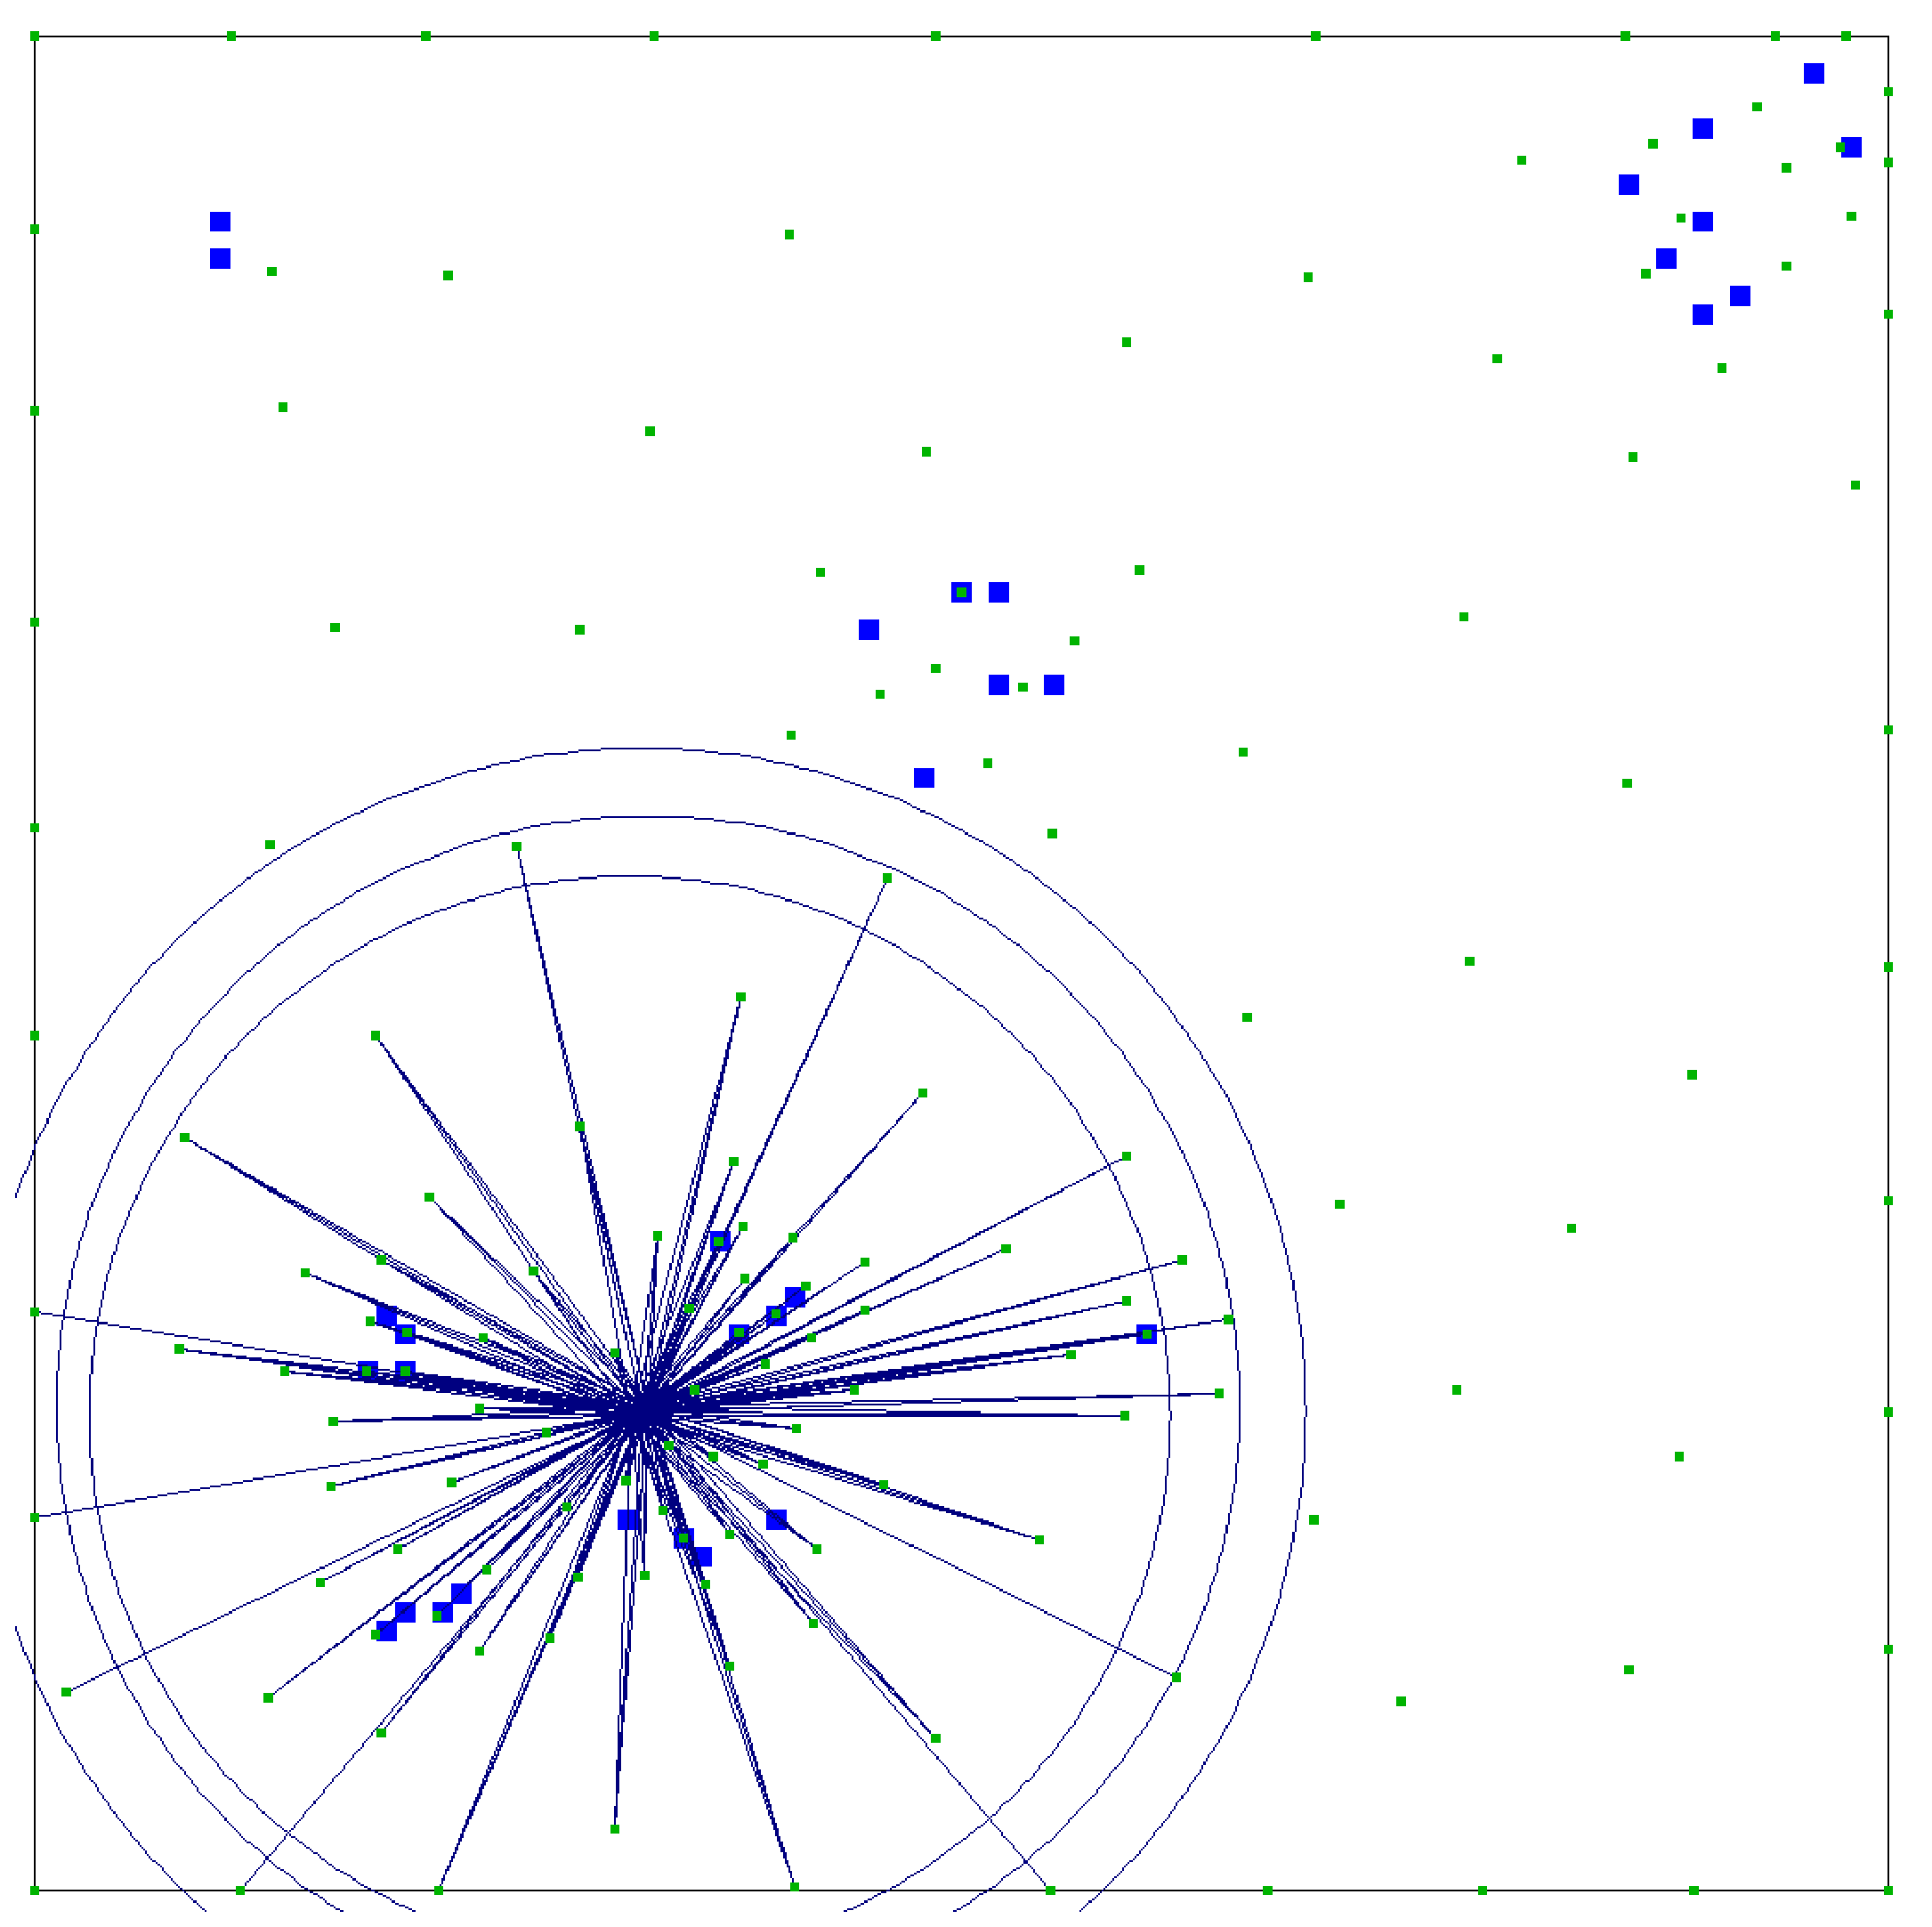
\includegraphics[width=0.6\textwidth]{img/places/share-all.eps}
  \caption{V�sledek testu vytv��en� m�st pro \eqref{formula:el-place-node-share} }
  \label{fig:el-place-node-share}
\end{figure}

To je zp�sobeno t�m, �e p��l� velkou ��st $\varrho(node)$ dostane m�sto s �rovn� jedna.
Definujme funkci $\varrho(node,misto)$ tak, aby uzel d�vat v�t�� ��st sv�ho $\varrho(node)$ t�m m�st�m, kter� jsou n�e v hiearchii, tj. maj� vy��� �rov��,
n�sleduj�c�m zp�sobem:
\begin{equation} 
\varrho(node,misto) = \varrho(node) \times  \frac{\displaystyle 2^{uroven(misto)} }{\displaystyle \sum_{\substack{
   m \in mista \\
   node \in m
  }} 2^{uroven(m)}
  }
\label{formula:el-place-node-share-exp}
\end{equation}

\begin{figure}[p]
  \centering
  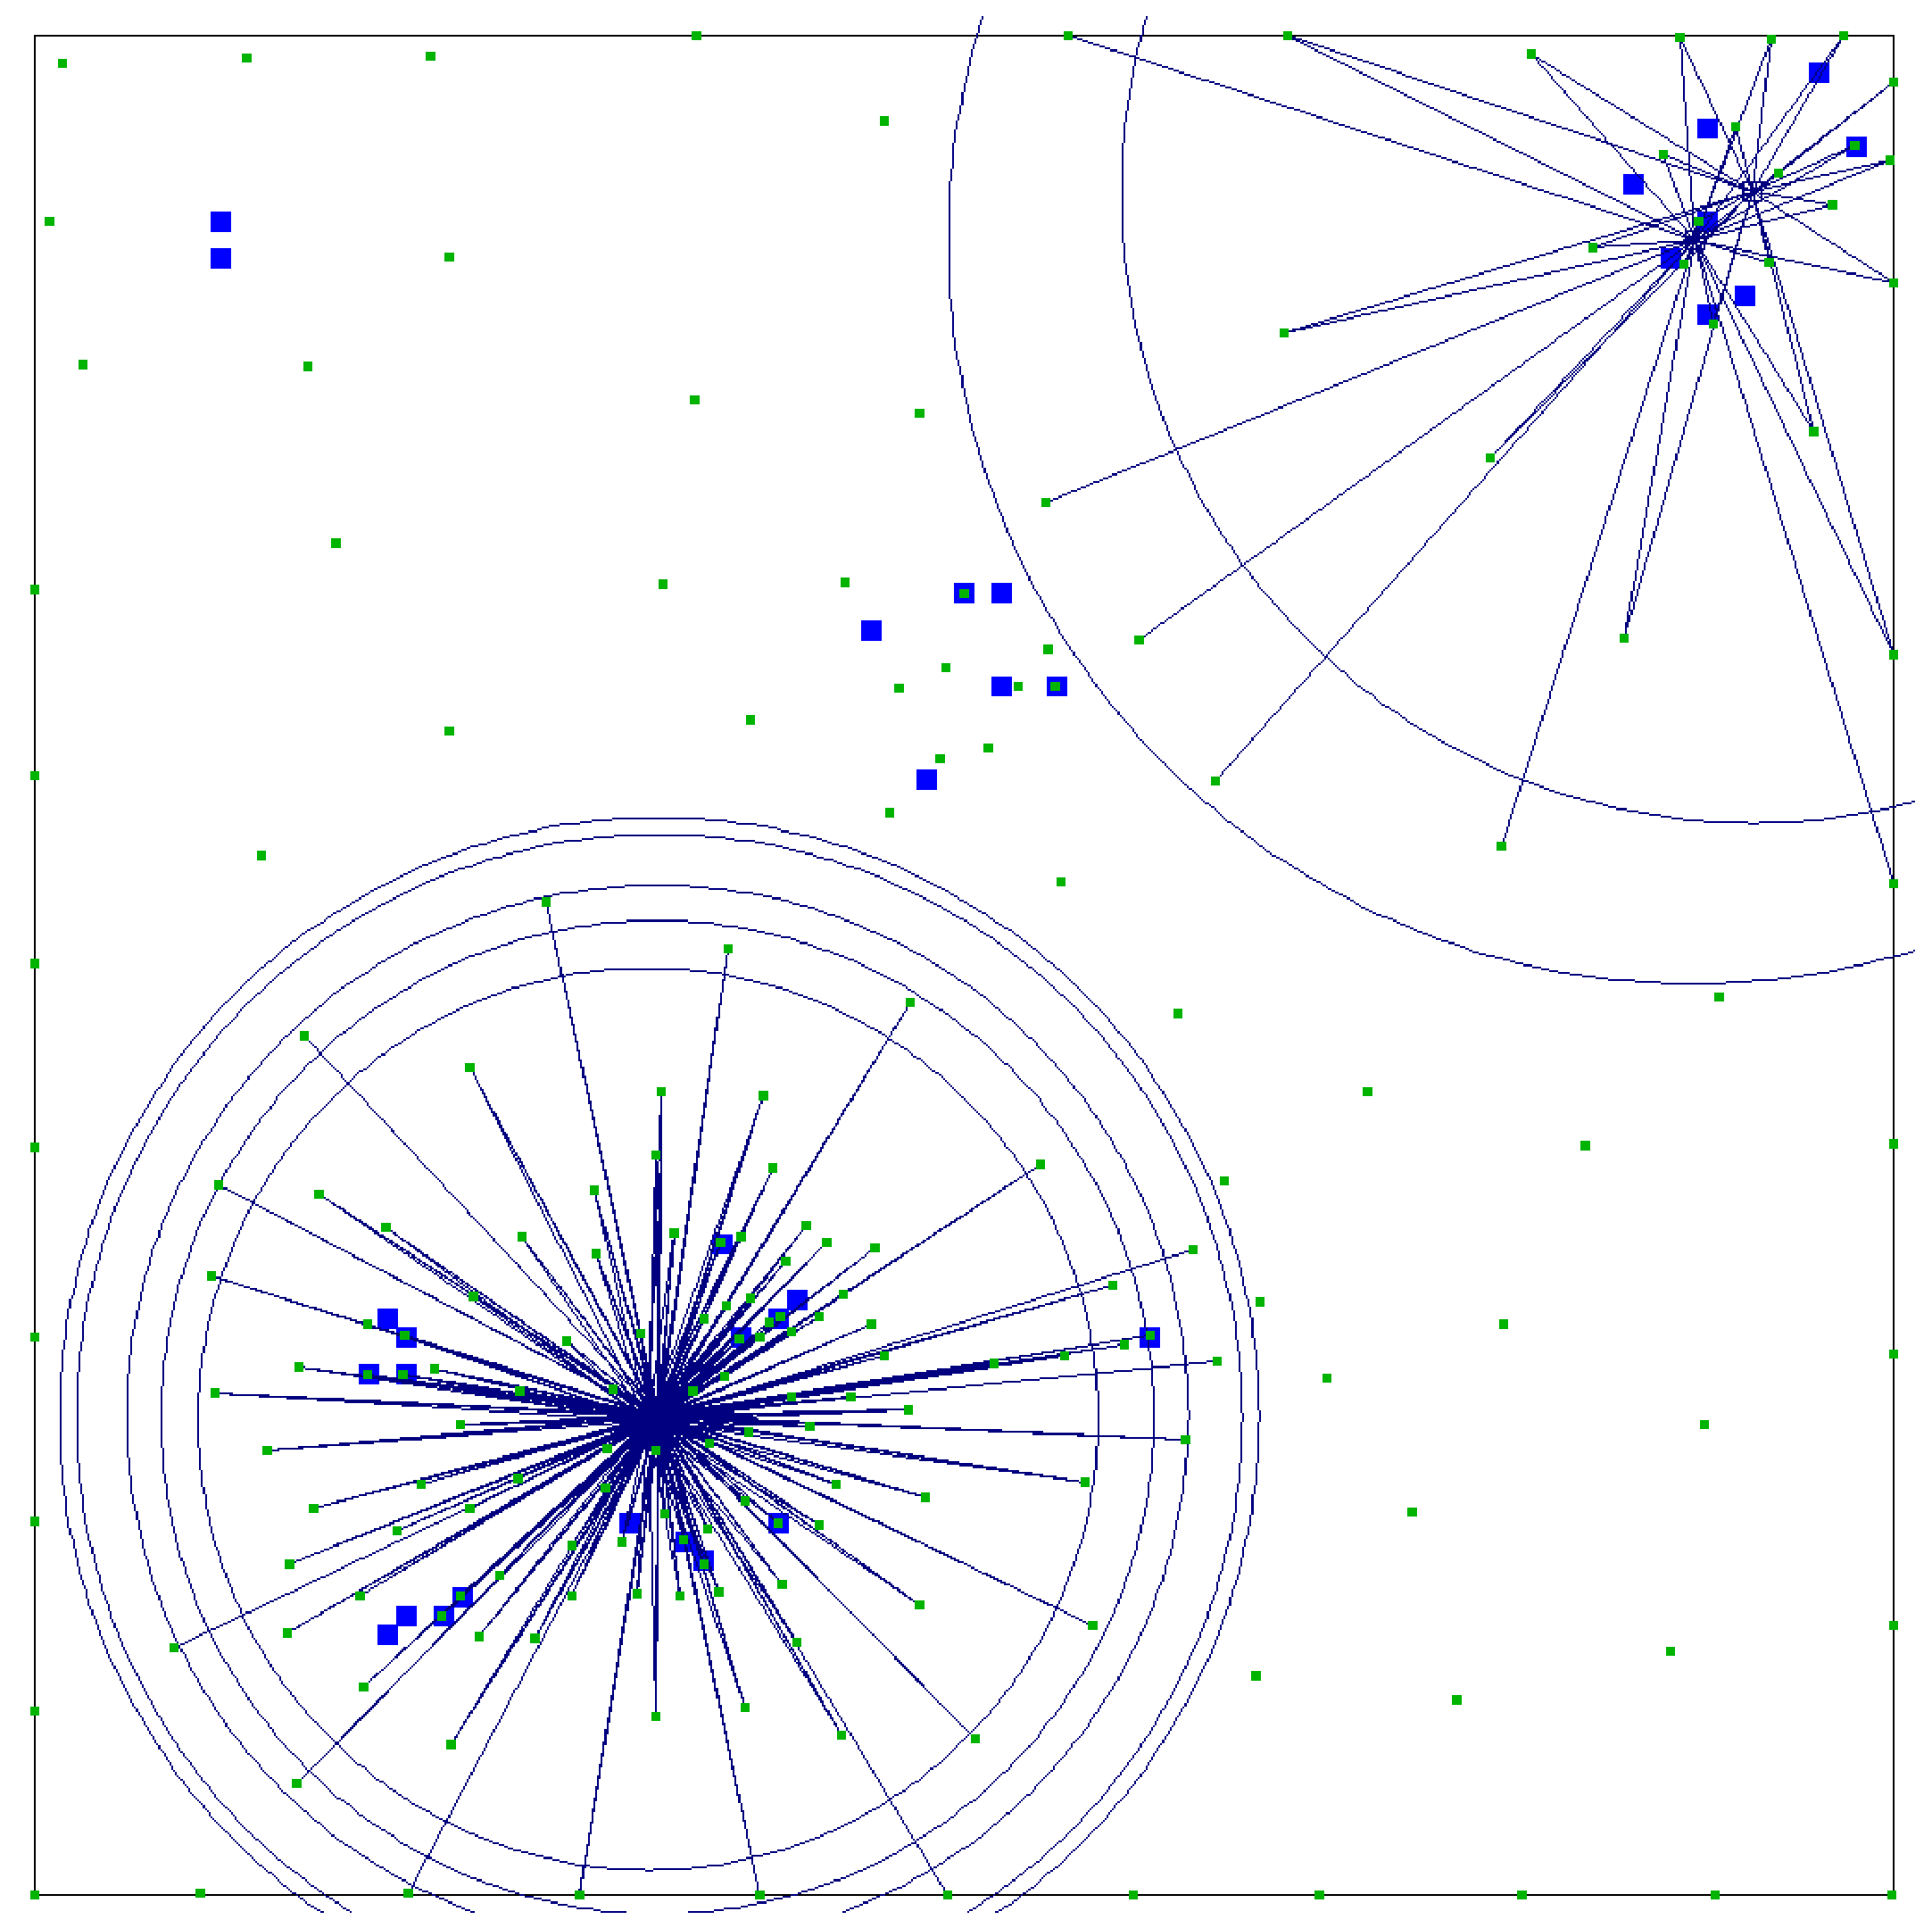
\includegraphics[width=0.6\textwidth]{img/places/share-exp.eps}
  \caption{V�sledek testu vytv��en� m�st pro \eqref{formula:el-place-node-share-exp} }
  \label{fig:el-place-node-share-exp}
\end{figure}

V�sledek je na obr�zku \ref{fig:el-place-node-share-exp}. Ukazuje, �e ani exponenci�ln� z�vislost na �rovni m�sta nezabr�n� p�ekr�v�n� m�st.
Pokud definujme funkci $\varrho(node,misto)$ tak, aby uzel rozd�loval rovnom�rn� sv� $\varrho(node)$ pouze m�st�m s nejvy���
�rovn� \footnote{Stejn� jako v \eqref{formula:el-place-node-share}, ale mno�ina ve jmenovateli bude obsahovat pouze m�sta s nejvy��� �rovn�},
dos�hneme stejn�ho v�sledku, viz obr�zek \ref{fig:el-place-node-share-maxlevel}.
\\

\begin{figure}[p]
  \centering
  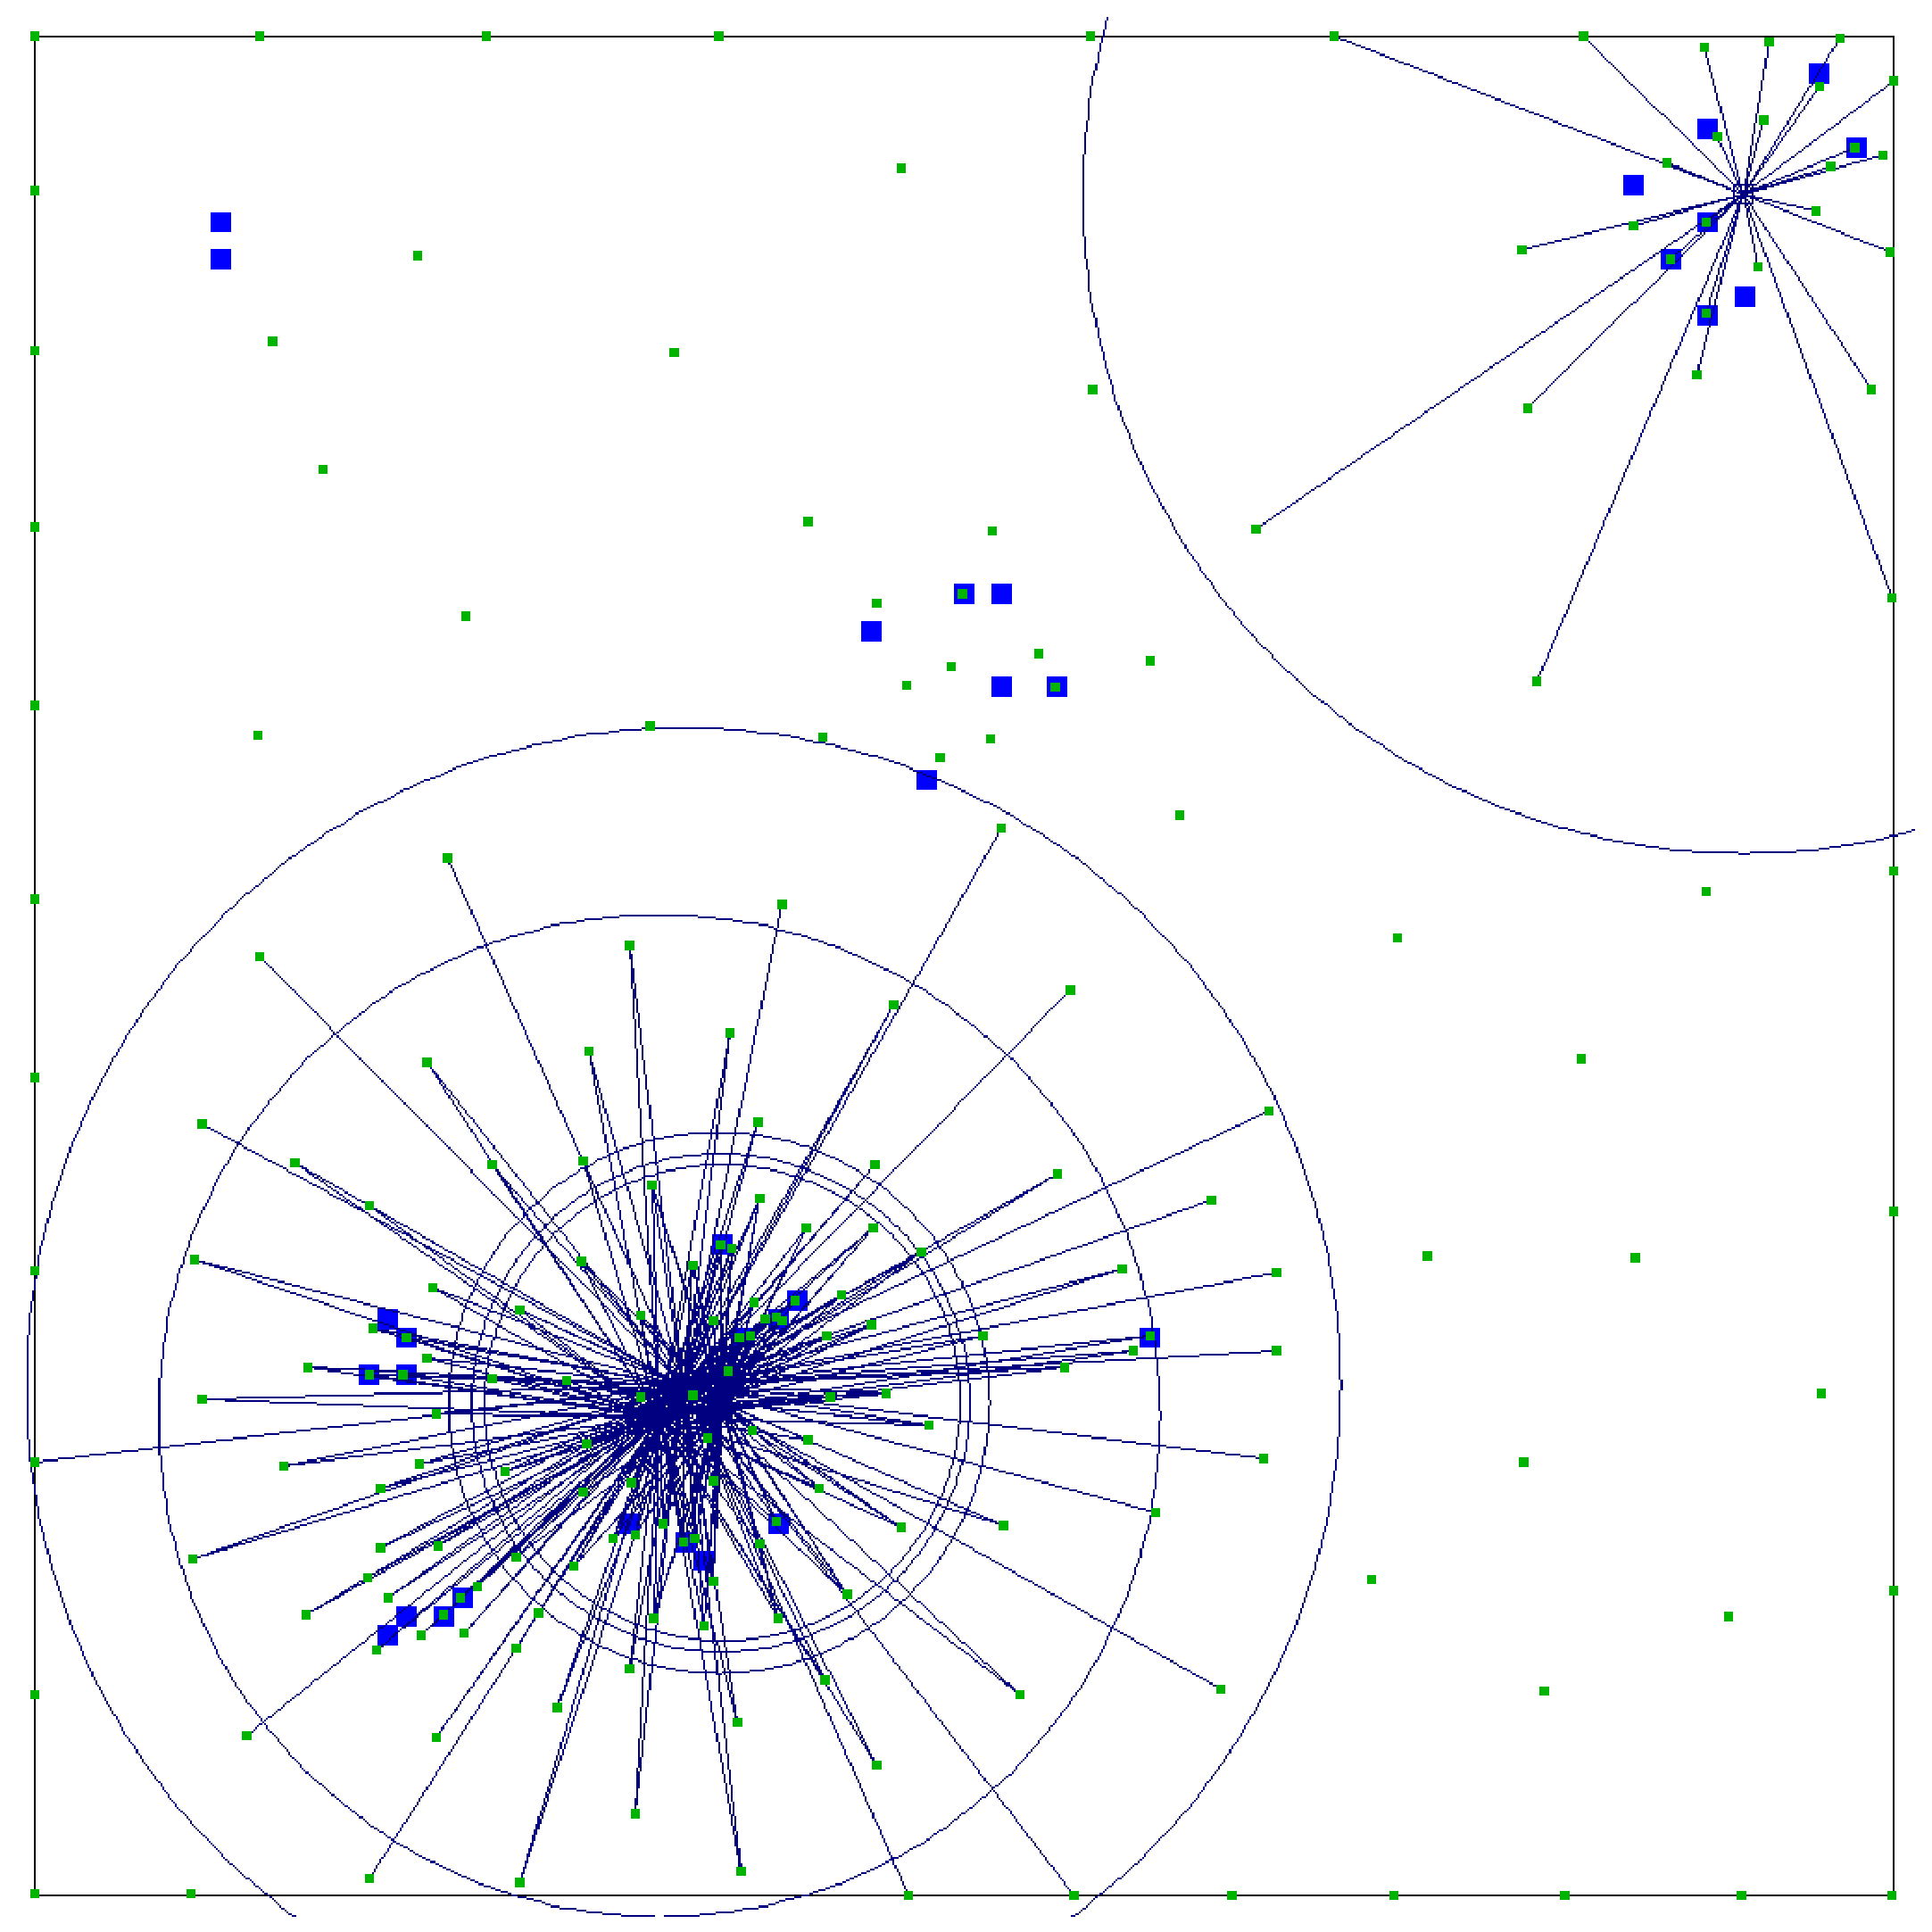
\includegraphics[width=0.6\textwidth]{img/places/share-maxlevel.eps}
  \caption{V�sledek testu vytv��en� m�st, kdy� uzel d�v� $\varrho(node)$ pouze uzl�m nejvy��� �rovn�.}
  \label{fig:el-place-node-share-maxlevel}
\end{figure}


Toto p�ekr�v�n� m�st je zp�sobeno t�m, �e $\varrho(node)$ je sd�leno v�ce m�sty.
Do modelu lze p�idat odpudivost m�st, to by v�ak model v�razn� zeslo�itilo.
Zkusili jsme p�ehodnotit n�le�en� uzlu do m�sta tak, aby ka�d� uzel n�le�el v�dy pr�v� jednomu m�stu.
�rove� m�sta je diskr�tn� veli�ina, kter� vyjad�uje jak malou oblast m�sto p�edstavuje.
Podobn� v�znam m� i polom�r m�sta, je to v�ak spojit� veli�ina, lze pomoc� n� tedy ur�it pr�v� jedno m�sto.
�ekn�m�, �e uzel n�le�� m�stu s nejmen��m polom�rem do kter�ho geometricky pat��:
\begin{equation} 
node \in misto \iff misto = \arg \min_{m \in mista(node)} polomer(m)
\label{formula:el-node-in-misto}
\end{equation}
\begin{equation} 
mista(node) = \{m \in mista ; dist(node,m) < polomer(m)\}
\label{formula:el-node-in-misto2}
\end{equation}
kde $mista$ je mno�ina v�ech m�st prostorov� mapy.
Pak m��eme definovat mno�stv� odpudivosti m�sta jednodu�eji ne� v \eqref{formula:el-agamount-mista-geo}, pouze jako sou�et:

\begin{equation} 
\varrho(misto) = \sum_{n \in misto} \varrho(node)
\label{formula:el-agamount-mista}
\end{equation}

Provedli jsme je�t� �pravu ur�en� polom�ru v z�vislosti na jeho intenzit�.
Chceme, aby polom�r m�sta se p�ilis nem�nil a plnil tak roli �rovn� m�sta v okam�iku, kdy ur�ujeme, kter� uzly do m�sta pat��.
Zm�nili jsme tedy koeficienty v \ref{formula:el-misto-range} na:

\begin{equation} 
polomer(misto) = polomer_0(misto) \times \left( \frac{1}{5} \times \frac{\eta_0(misto)}{\eta(misto)} + \frac{4}{5} \right)
\label{formula:el-misto-range-new}
\end{equation}

V�sledek testu je na obr�zku \ref{fig:el-place-node-share-one}.
Na jeho z�klad�\footnote{A na z�klad� dal��ch test�, kter� lze nal�zt na p�ilo�en�m CD.} pova�ujeme toto �e�en� za vyhovuj�c�.

\begin{figure}[h!]
  \centering
  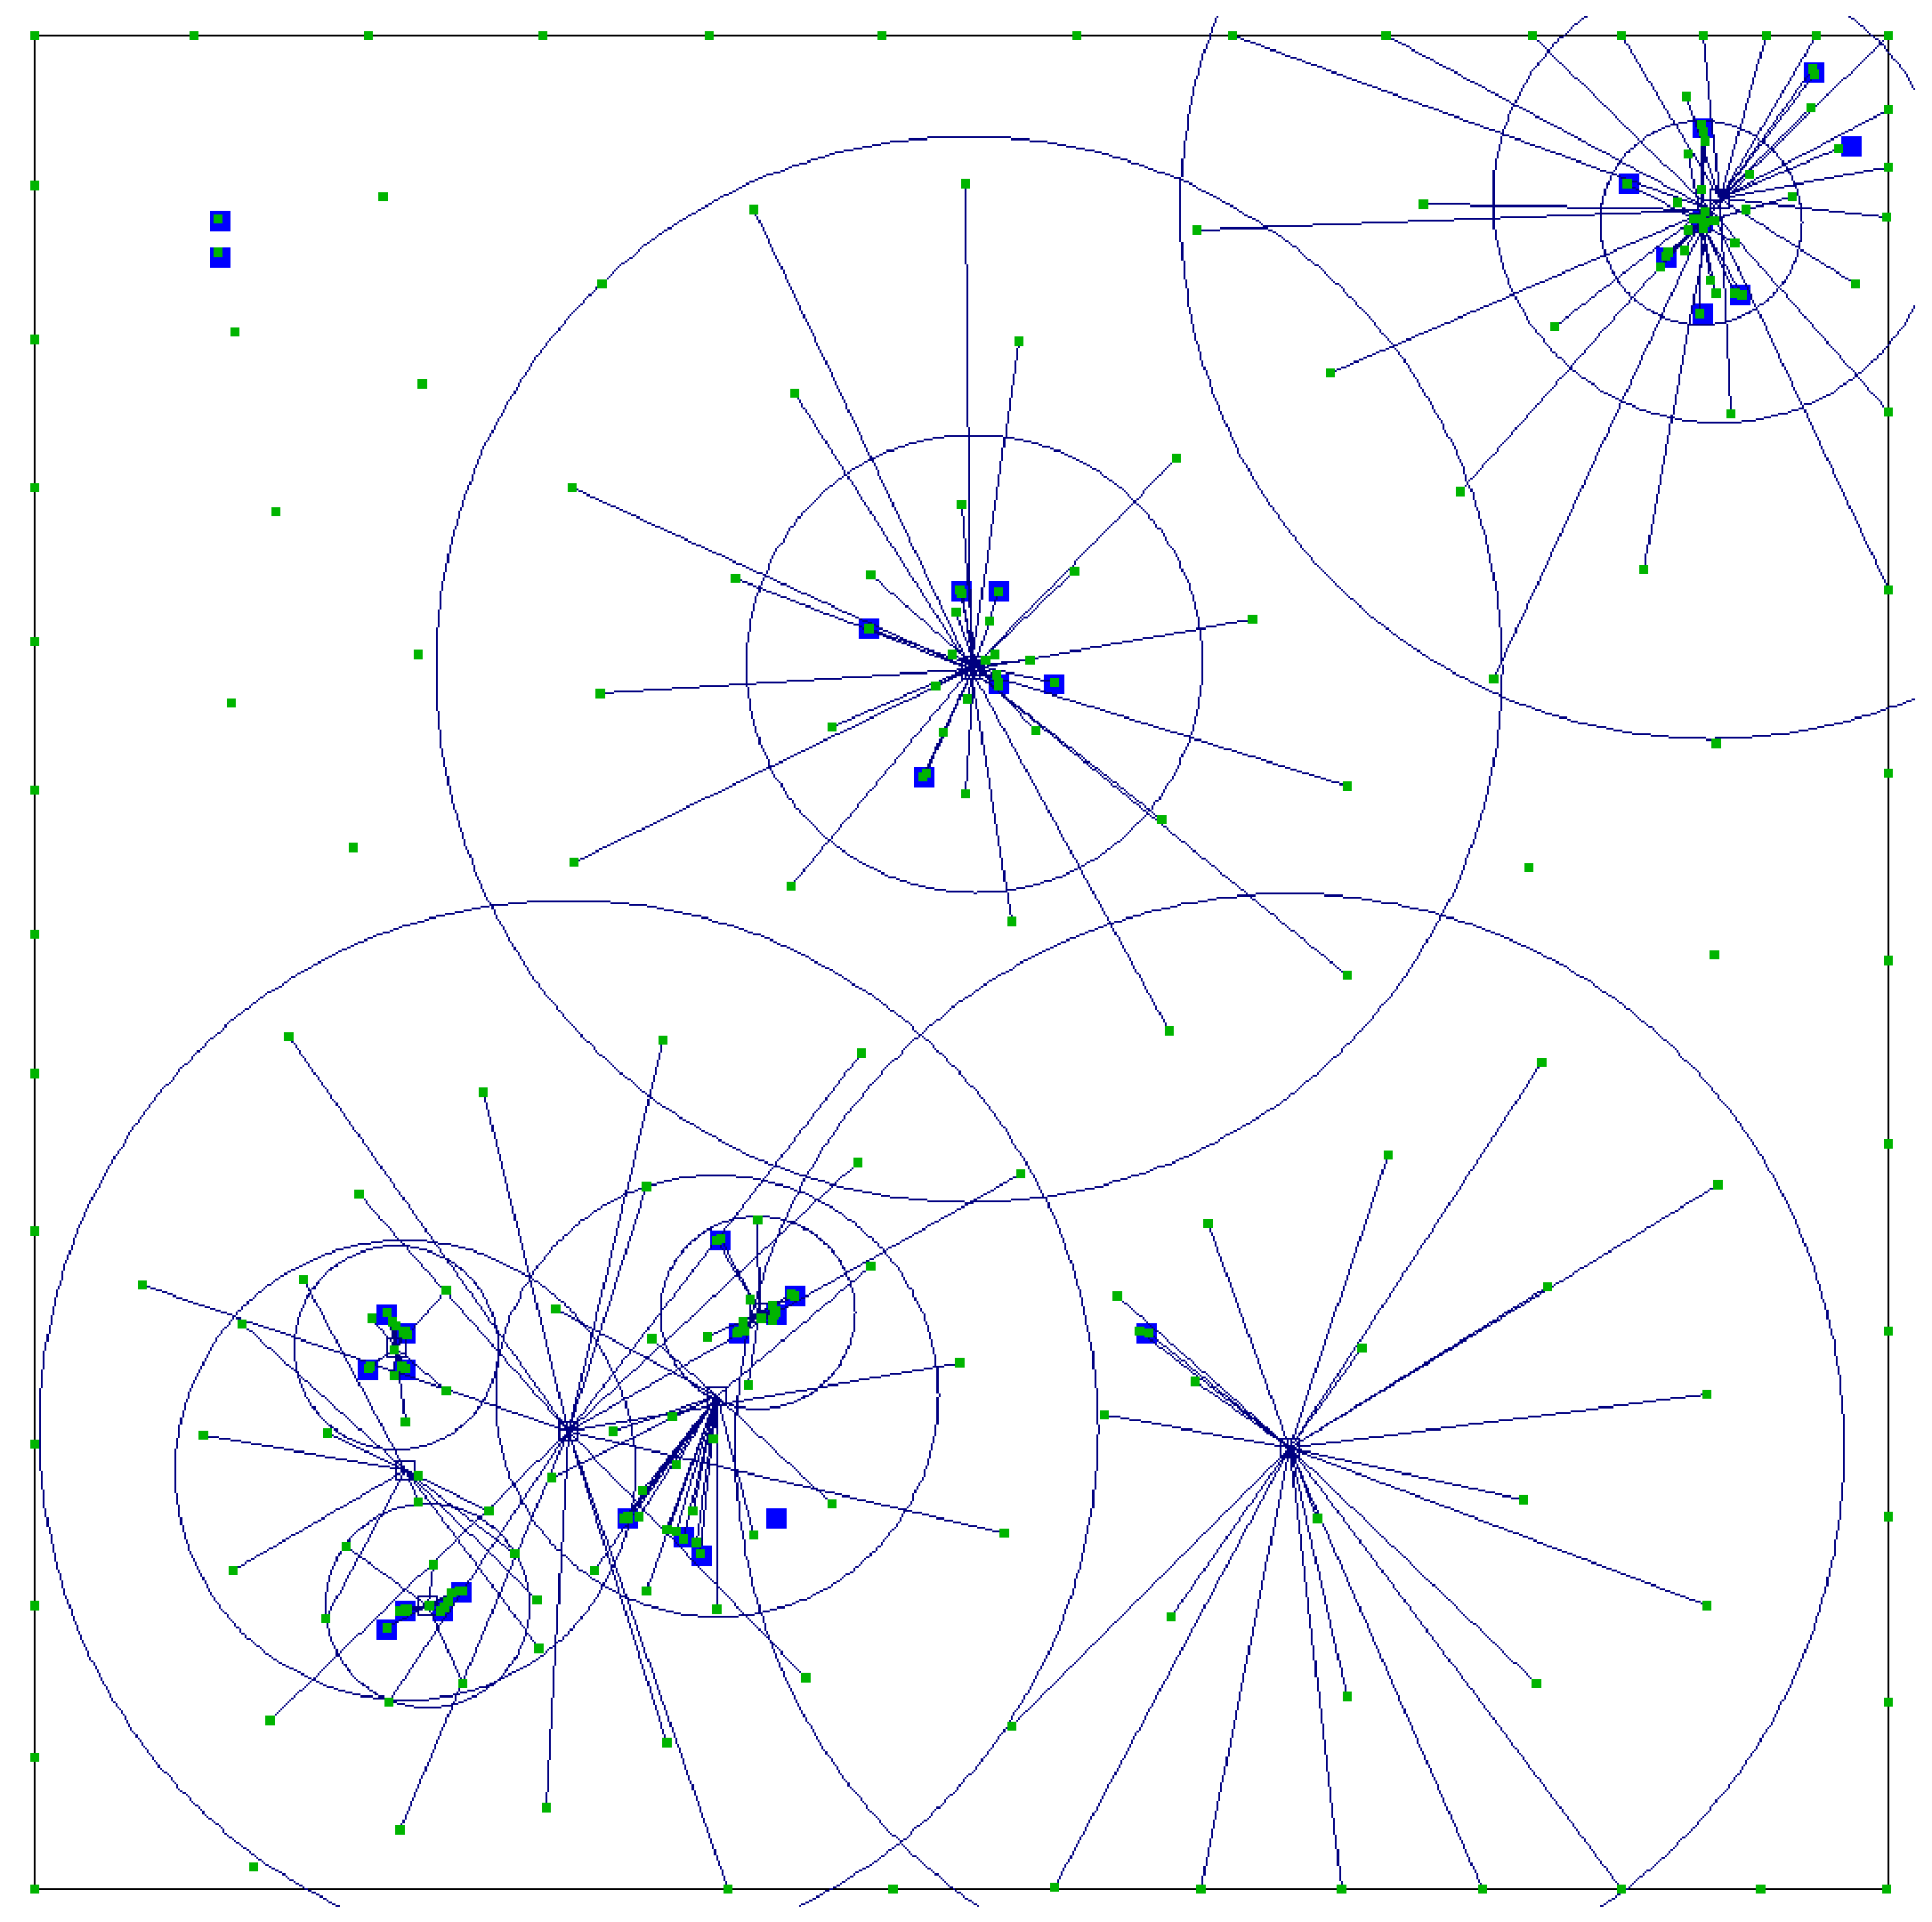
\includegraphics[width=0.6\textwidth]{img/places/share-one.eps}
  \caption{V�sledek testu vytv��en� m�st, kdy� uzel n�le�� pr�v� jednomu m�stu. Dva p�edm�ty v lev�m horn�m rohu agent v pr�b�hu simulace nikdy nepou�il a pouze n�kolikr�t vid�l.}
  \label{fig:el-place-node-share-one}
\end{figure}



% SHRNUTI - PREHLED %%%%%%%%%%%%%%%%%%%%%%%%%%%%%%%%%%%%%%%%%%%%%%%%%%%%%%%%%%%%%%%%%%%%%%%%%%%%%%%%%%%%%%%%%%%%%%%%%%%%%%%%%%%%%%%%%%%%%%%%%%%


\subsection{V�sledn� model a slo�itost algoritm�}

V p�edch�zej�c�ch kapitol�ch byl postupn� p�edstaven gravita�n� model v�etn� r�zn�ch variant a slep�ch v�vojov�ch v�tv�.
Tato kapitola shrnuje v�sledn� model.
Gravita�n� model vrstvy uzl� m� t�i hlavn� ��sti: \emph{vytvo�en� prvotn� mapy}, \emph{zpracov�n� vjemu} a \emph{aktualizace mapy}.
\\

Vytvo�en� mapy je pops�no v kapitole \ref{chapter-createmap}.
Jeho �asov� slo�itost z�vis� pouze na velikost m�stsnoti, pro kterou je vytv��ena, je line�rn� v po�tu uzl�, kter� je t�eba vytvo�it.
Zpracov�n� vjemu znamen� pouze vytvo�en� stopy vjemu �i zv��en� intenzity ji� existuj�c� stopy vjemu dle vzorce \eqref{formula:el-stopa-start-int}.
Samotn� vytvo�en� stopy vjemu �i zv��en� intenzity m� konstantn� �asovou slo�itost.
N�ro�n�j�� je ur�it, zda v dan� poloze u� n�jak� stopa vjemu je.
Sta�� proj�t seznam v�ech existuj�c�ch stop vjemu a porovnat jejich polohy, tento algoritmus m� line�rn� �asovou slo�itost vzhledem k po�tu existuj�c�ch stop vjemu.
Jejich po�et je omezen velikost� percep�n�ho pole a kr�tkou �ivotnost�, typicky existuje sou�asn� nejv��e kolem 10 stop vjemu.
\\

Nejn�ro�n�j�� ��st� je aktualizce mapy. Skl�d� se z n�sleduj�c�ch ��st�:
\emph{aktualizace stop vjemu}, \emph{aktualizace uzl� mapy}, \emph{aktualizace m�st}, \emph{zapom�n�n� uzl�}.

\subsubsection{Aktualizace stop vjemu}
Jedn� se o algoritmy \ref{alg:stopa-step} a \ref{alg:stopa-step-create}, kter� jsou postupn� provedeny nad v�emi existuj�c�mi stopami vjemu.
\\

Algoritmus \ref{alg:stopa-step} obsahuje dva cykly, po�et opakov�n� je roven po�tu okoln�ch uzl� $\mid nodes_{around}\mid$.
T�la obou cykl� jsou konstatn� operace. V druh�m cyklu je sice pou�it vzorec \eqref{formula:el-intenzita}, kter� obsahuje sumu p�es v�echny okoln� uzly,
jej� hodnota se v�ak nem�n� a je mo�n� ji p�edpo��tat v line�rn�m �ase.
Mno�inu $nodes_{around}$ okoln�ch uzl� lze ur�it v �ase $O(n_c)$, kde $n_c$ je po�et uzl� mapy.
Proto�e plat� $\mid nodes_{around}\mid < n_c$, je v�sledn� �asov� slo�itost algoritmu pro jednu stopu vjemu $O(n_c)$.
\\

Algoritmus \ref{alg:stopa-step-create} obsahuje pouze operace s konstantn� �asovou slo�itost�.
Pokud je vytvo�en nov� uzel, je nutn� ur�it m�sto, do kter�ho n�le��. To v�ak lze prov�st a� v r�mci aktualizace m�st.
Cenu uzlu ur�uje vzorec \eqref{formula:cost-create-sum}.
\\

V�sledn� slo�itost algoritmu, kter� aktualizuje v�echny stopy vjemu, je $O(n_c \times s_c)$, kde $s_c$ je po�et stop vjemu.
\\


\subsubsection{Aktualizace uzl� mapy}
V ka�d�m kroku simulace je ur�ena vz�jemn� odpudivost uzl�. To znamen� spo��t�n� vzd�lenosti mezi v�emi uzly.
Ur�en� odpudivost mezi dv�ma uzly m� konstantn� �asovou slo�itost.
Spo�ten� v�ech odpudiv�ch sil m� tedy �asovou slo�itost $O(n_c^2)$.
\\

Spo�ten� odpudiv� s�ly jsou prom�tnuty do mno�stv� odpudivost uzlu dle vzorce \eqref{formula:el-agamount}.
\\


\subsubsection{Aktualizace m�st}
V ka�d�m kroku simulace je nad ka�d�m m�stem proveden algoritmus \ref{alg:el-step-misto}.
Pak je pro ka�d� uzel mapy ur�eno, do jak�ho m�sta n�le�� dle vzorce \eqref{formula:el-node-in-misto}.
Pro ur�en� mno�stv� odpudivosti m�sta je v kroku \ref{alg:el-step-misto-varrho} pou�it vzorec \label{formula:el-agamount-mista},
v kroku \label{alg:el-step-misto-polomer} je pou�it vzorec \eqref{formula:el-misto-range-new}.
Pokud je mno�stv� odpudivosti m�sta v�t�� ne� limit dan� modelem, jsou vytvo�ena dal�� podm�sta algoritmem \ref{alg:el-misto-split}.
\\

V�t�ina krok� algoritmu \ref{alg:el-step-misto} m� konstantn� �asovou slo�itost,
kroky \ref{alg:el-step-misto-varrho} a \ref{alg:el-step-misto-centroid} z�vis� na po�tu uzl� a podm�st, kter� m�sto obsahuje.
Tyto kroky lze prov�st najednou pro v�echna m�sta jedn�m pr�chodem do ���ky stromem m�st.
P�i tomto pr�chodu bude ka�d� uzel pou�it pr�v� jednou.
Pokud nedojde k vytvo�en� podm�st, m� aktualizace v�ech m�st prostorov� mapy line�rn� slo�itost $O(m_c \times n_{c})$, kde $m_c$ je po�et m�st mapy.
Ur�en� p��slu�nosti uzlu do m�sta m� stejnou �asovou slo�itost.
\\

Algoritmus \ref{alg:el-misto-split} je velmi podobn� jednomu kroku simulace m�sta.
Jeho �asov� slo�itost je line�rn� k po�tu uzl� v nad�azen�m m�st�, tj. lze ji omezit $O(n_c)$.
Algoritmus m��e b�t p�i jednom d�len� m�sta spu�t�n n�kolikr�t, maxim�ln� po�et spu�t�n� z�vis� na pod�lu parametr� modelu
\param{limit vzniku podm�sta} a \param{limit zapomenut� m�sta}.
\\


\subsubsection{Zapom�n�n� uzl�}
Zapom�n�n� uzl� je pops�no algoritmem \ref{alg:node-forget}.
Algoritmus m� konstantn� �asovou slo�itost a� na proveden� lok�ln�ch krok� simulace.
Ty znamenaj� po��t�n� odpudivosti mezi uzly a lze je omezit $O(n_c^2)$.
V ka�d�m kroku je zapomenut nejv��e jeden uzel, po�et kroku je parametr modelu, tedy konstanta.
\\

\subsubsection{Slo�itost kroku simulace}
V ka�d�m kroku simulace je provedena aktualizace mapy, kter� m� v��e uveden� ��sti.
Celkov� slo�itost jednoho kroku simulace je $O(n_c^2)$. P�edpokl�d�me, �e:
$s_c \ll n_c$ a $m_c \ll n_c$.

%$O(n_c,s_c)$ - stopy
%$O(n_c^2)$ - uzly
%$O(m_c, n_{c})$ - mista
%$O(n_c^2)$ - forget


\chapter{V�sledky test� modelu}

Tato kapitola obsahuje v�sledky test� modelu.
V prvn� podkapitole jsou testy fin�ln�ho modelu prostorov� mapy na r�zn�ch datech, v dal��ch jsou testy modelu s r�zn�mi hodnotami n�kter�ch kl��ov�ch parametr�.
\\

Samotn� test je ur�en testovac�m sv�tem\footnote{P�ehled v�ech testovac�ch m�stnost� je v p��loze A.},
tedy m�stnost� a sc�n��em a hodnotami parametr�.
\\


\section{Testy v�sledn�ho modelu} \label{chapter-test-final}
Model prostorov� mapy popsan� v kapitole \ref{chapter-model} resp. \ref{chapter-model-el}
s v�choz�m nastaven�m parametr� dle tabulky \ref{tab:param-el} v p��loze B jsme otestovali v osmi r�zn�ch m�stnostech. 
Na obr�zku \ref{fig:final-crazy}, \ref{fig:final-heapline} a \ref{fig:final-lobby} jsou v�sledky ve t�ech m�stnostech.
V�sledky v dal��ch m�stnostech, dal�� v�stupn� data a videa zachycuj�c� pr�b�h test� jsou na p�ilo�en�m CD.
\\


\begin{figure}[p]
  \centering
  \subfloat[Krok 1000]{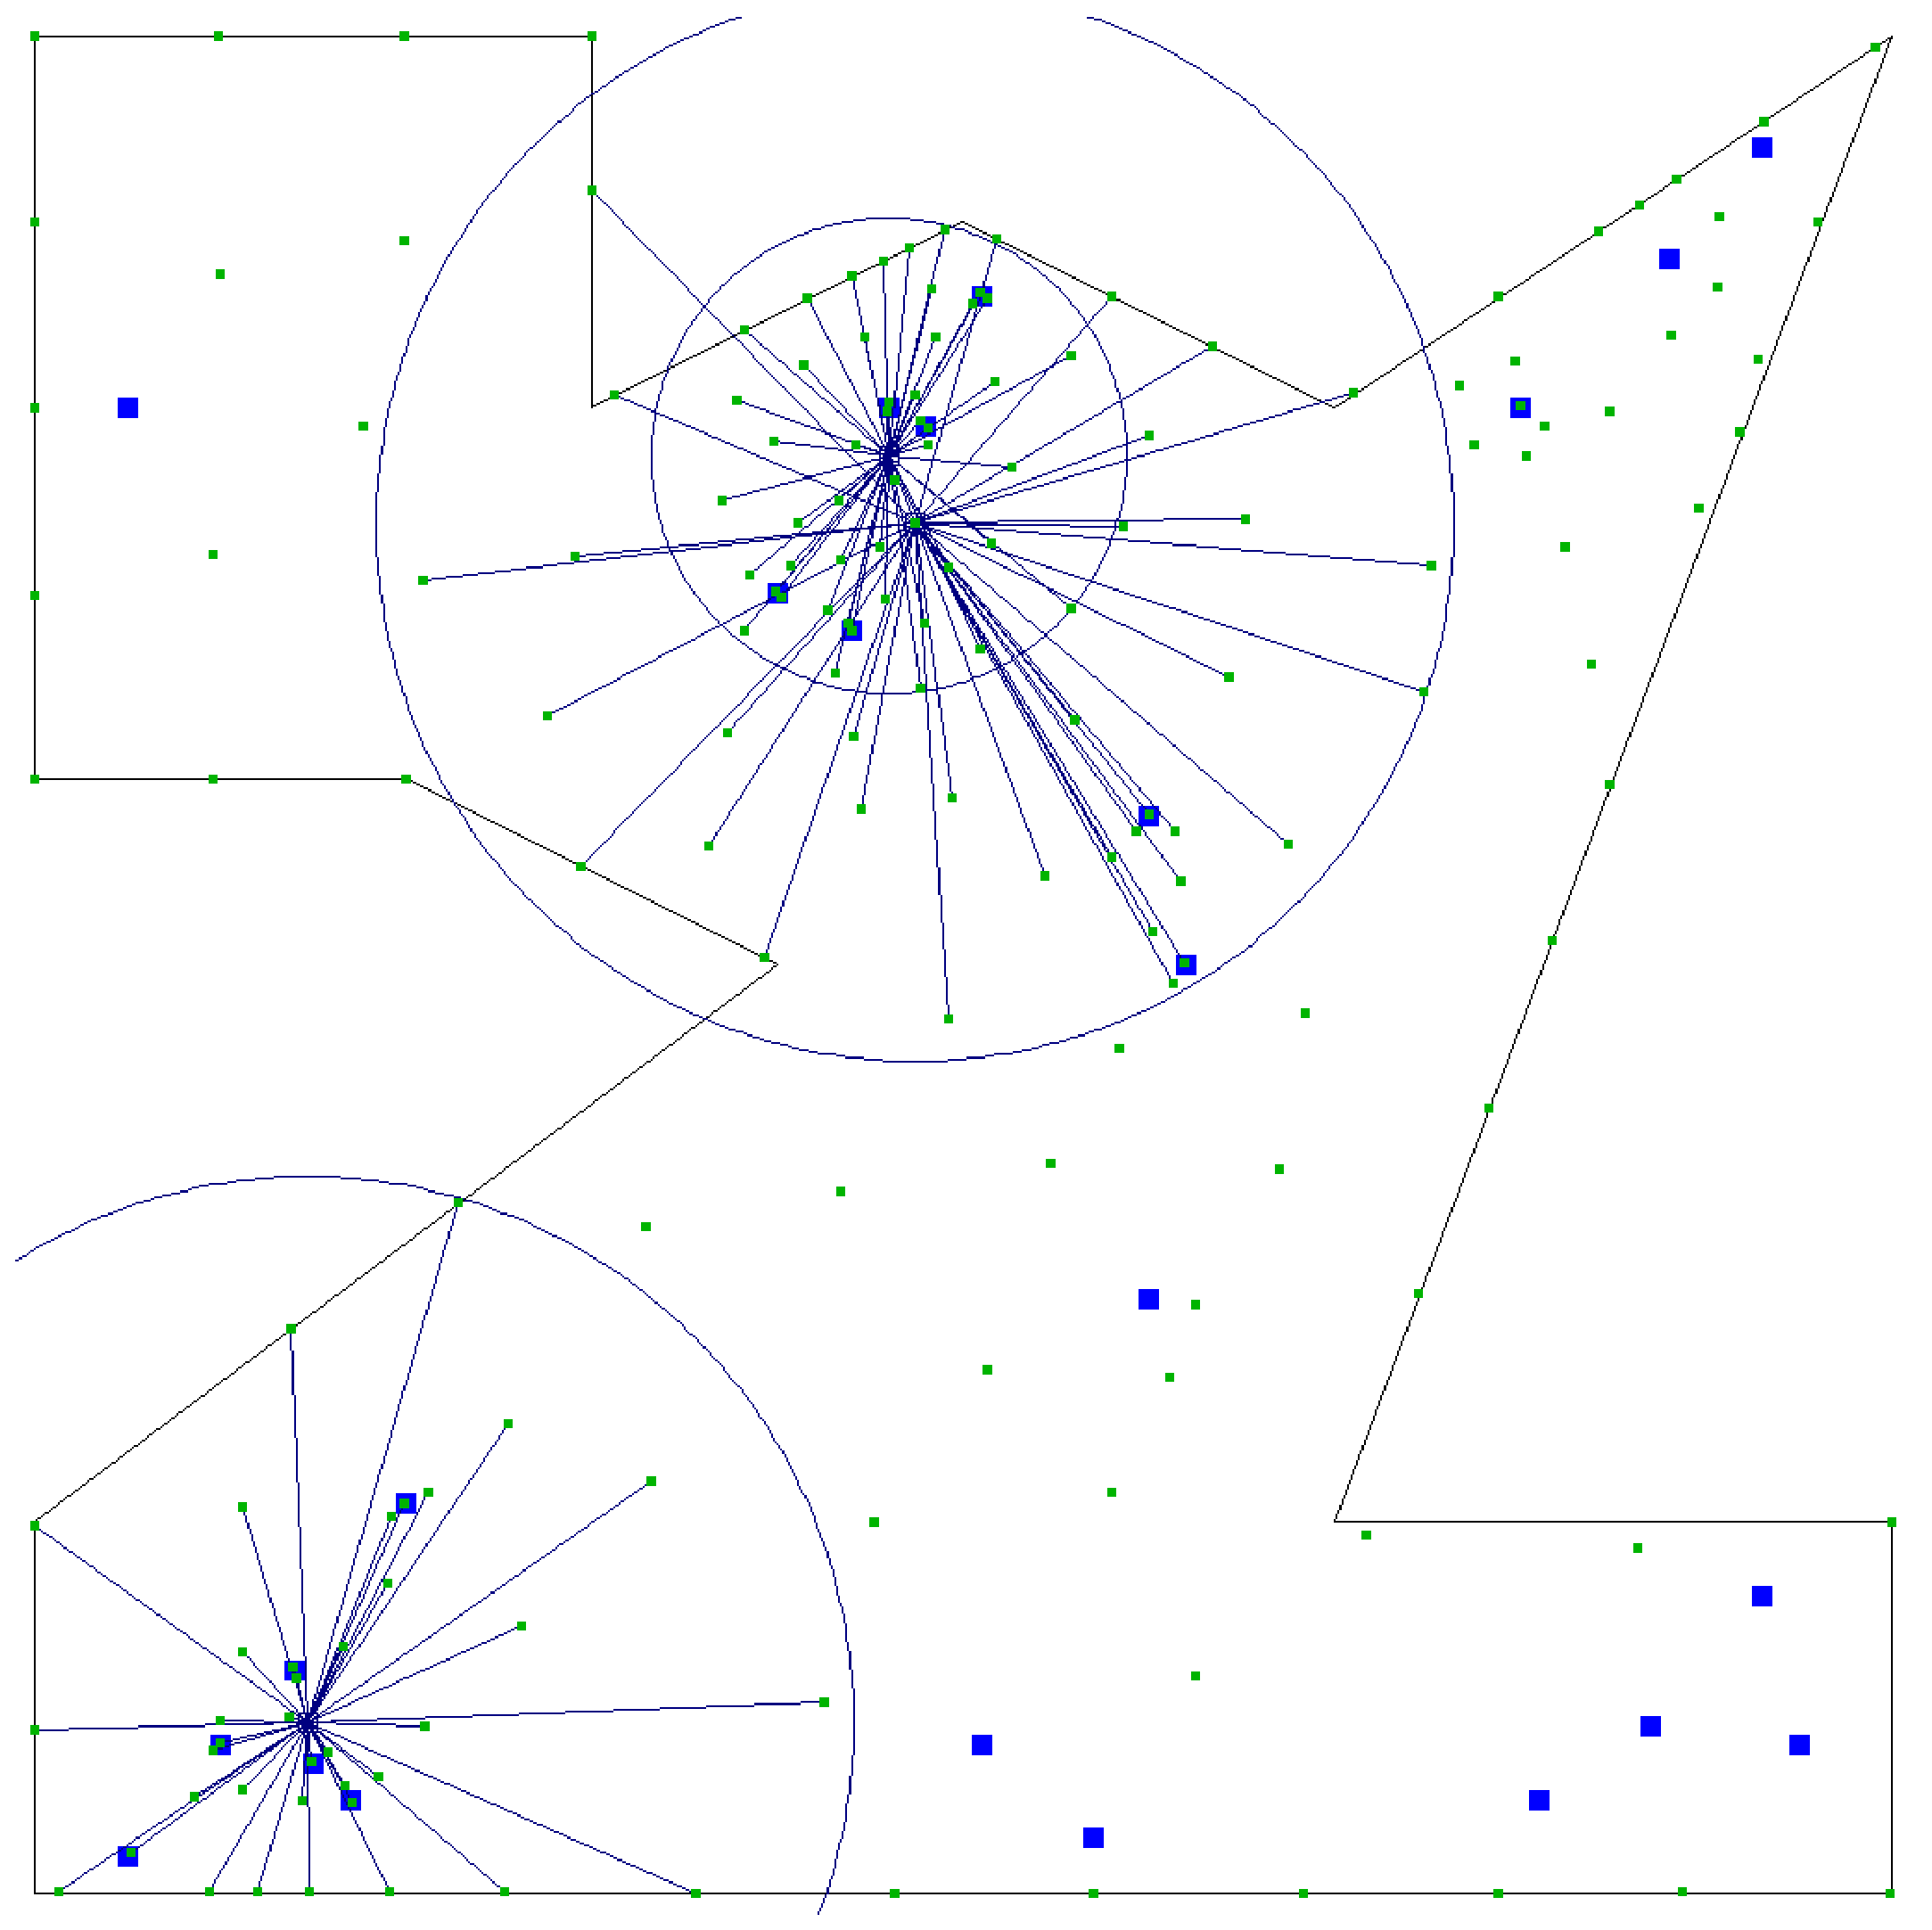
\includegraphics[width=0.5\textwidth]{img/final/crazy1000.eps}}
  \subfloat[Krok 5000]{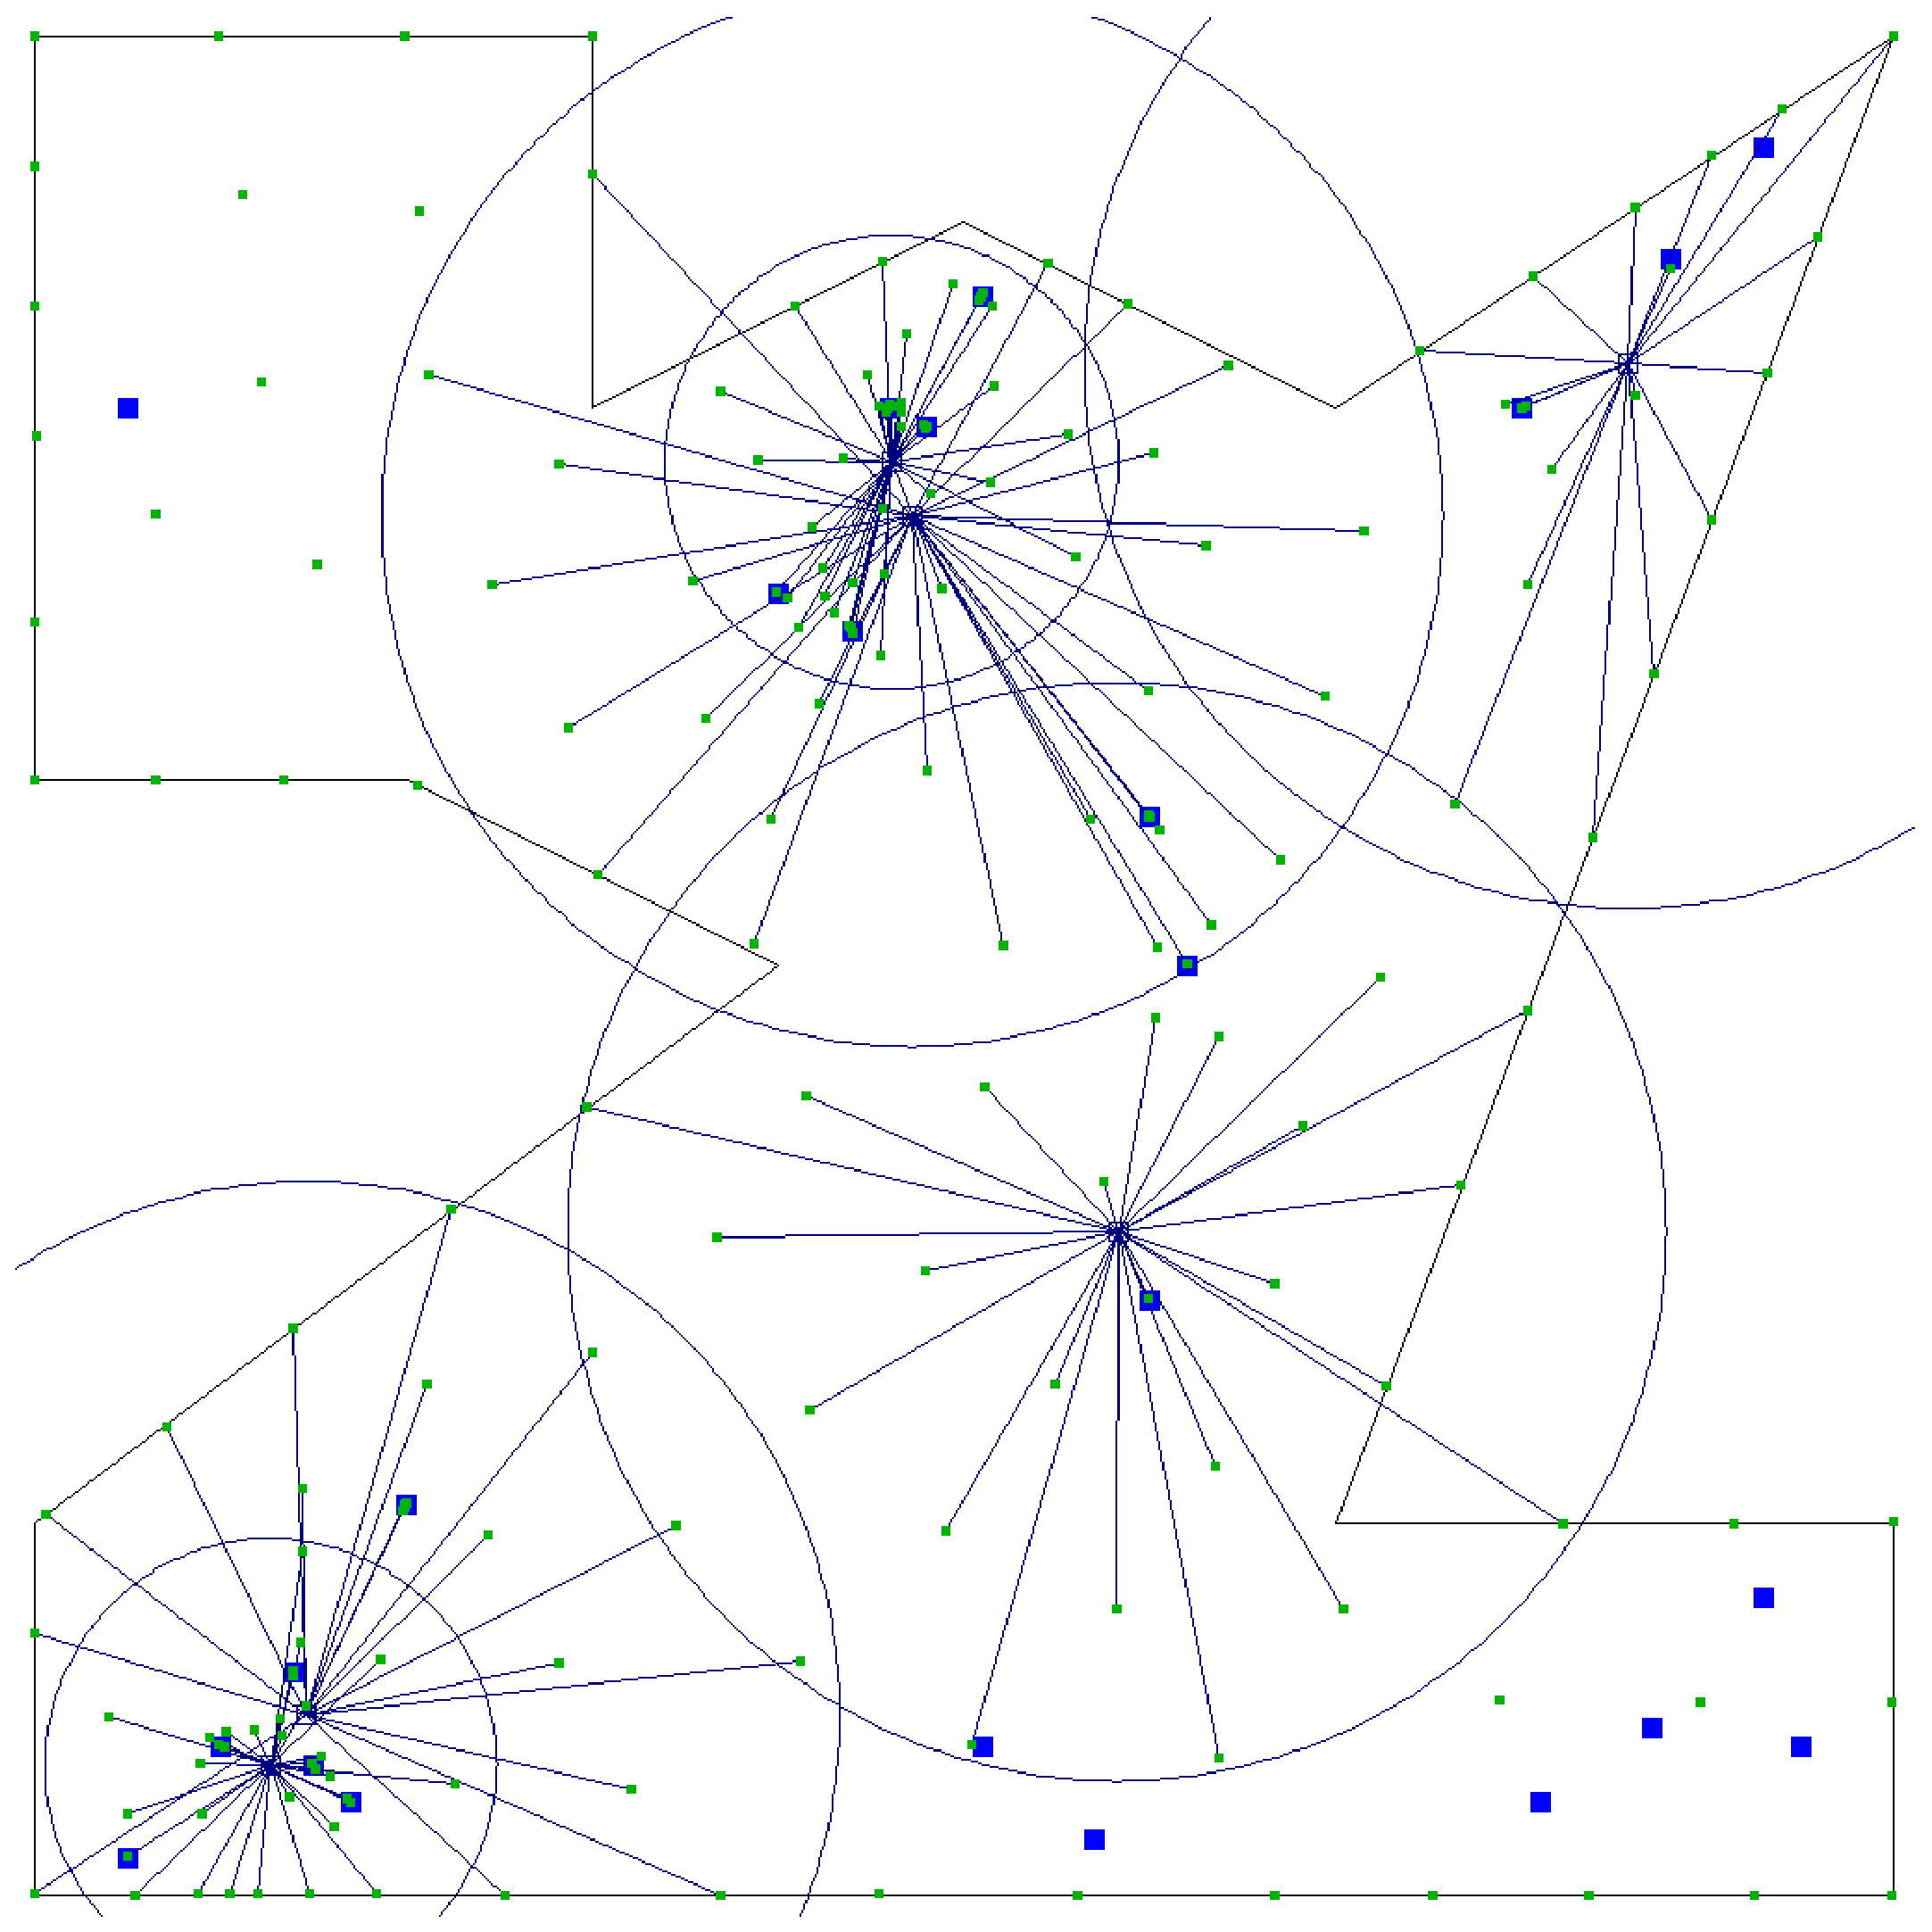
\includegraphics[width=0.5\textwidth]{img/final/crazy5000.eps}}
  \caption{Test v�sledn�ho modelu, m�stnost CrazyRoom.}
  \label{fig:final-crazy}
\end{figure}

\begin{figure}[p]
  \centering
  \subfloat[Krok 1000]{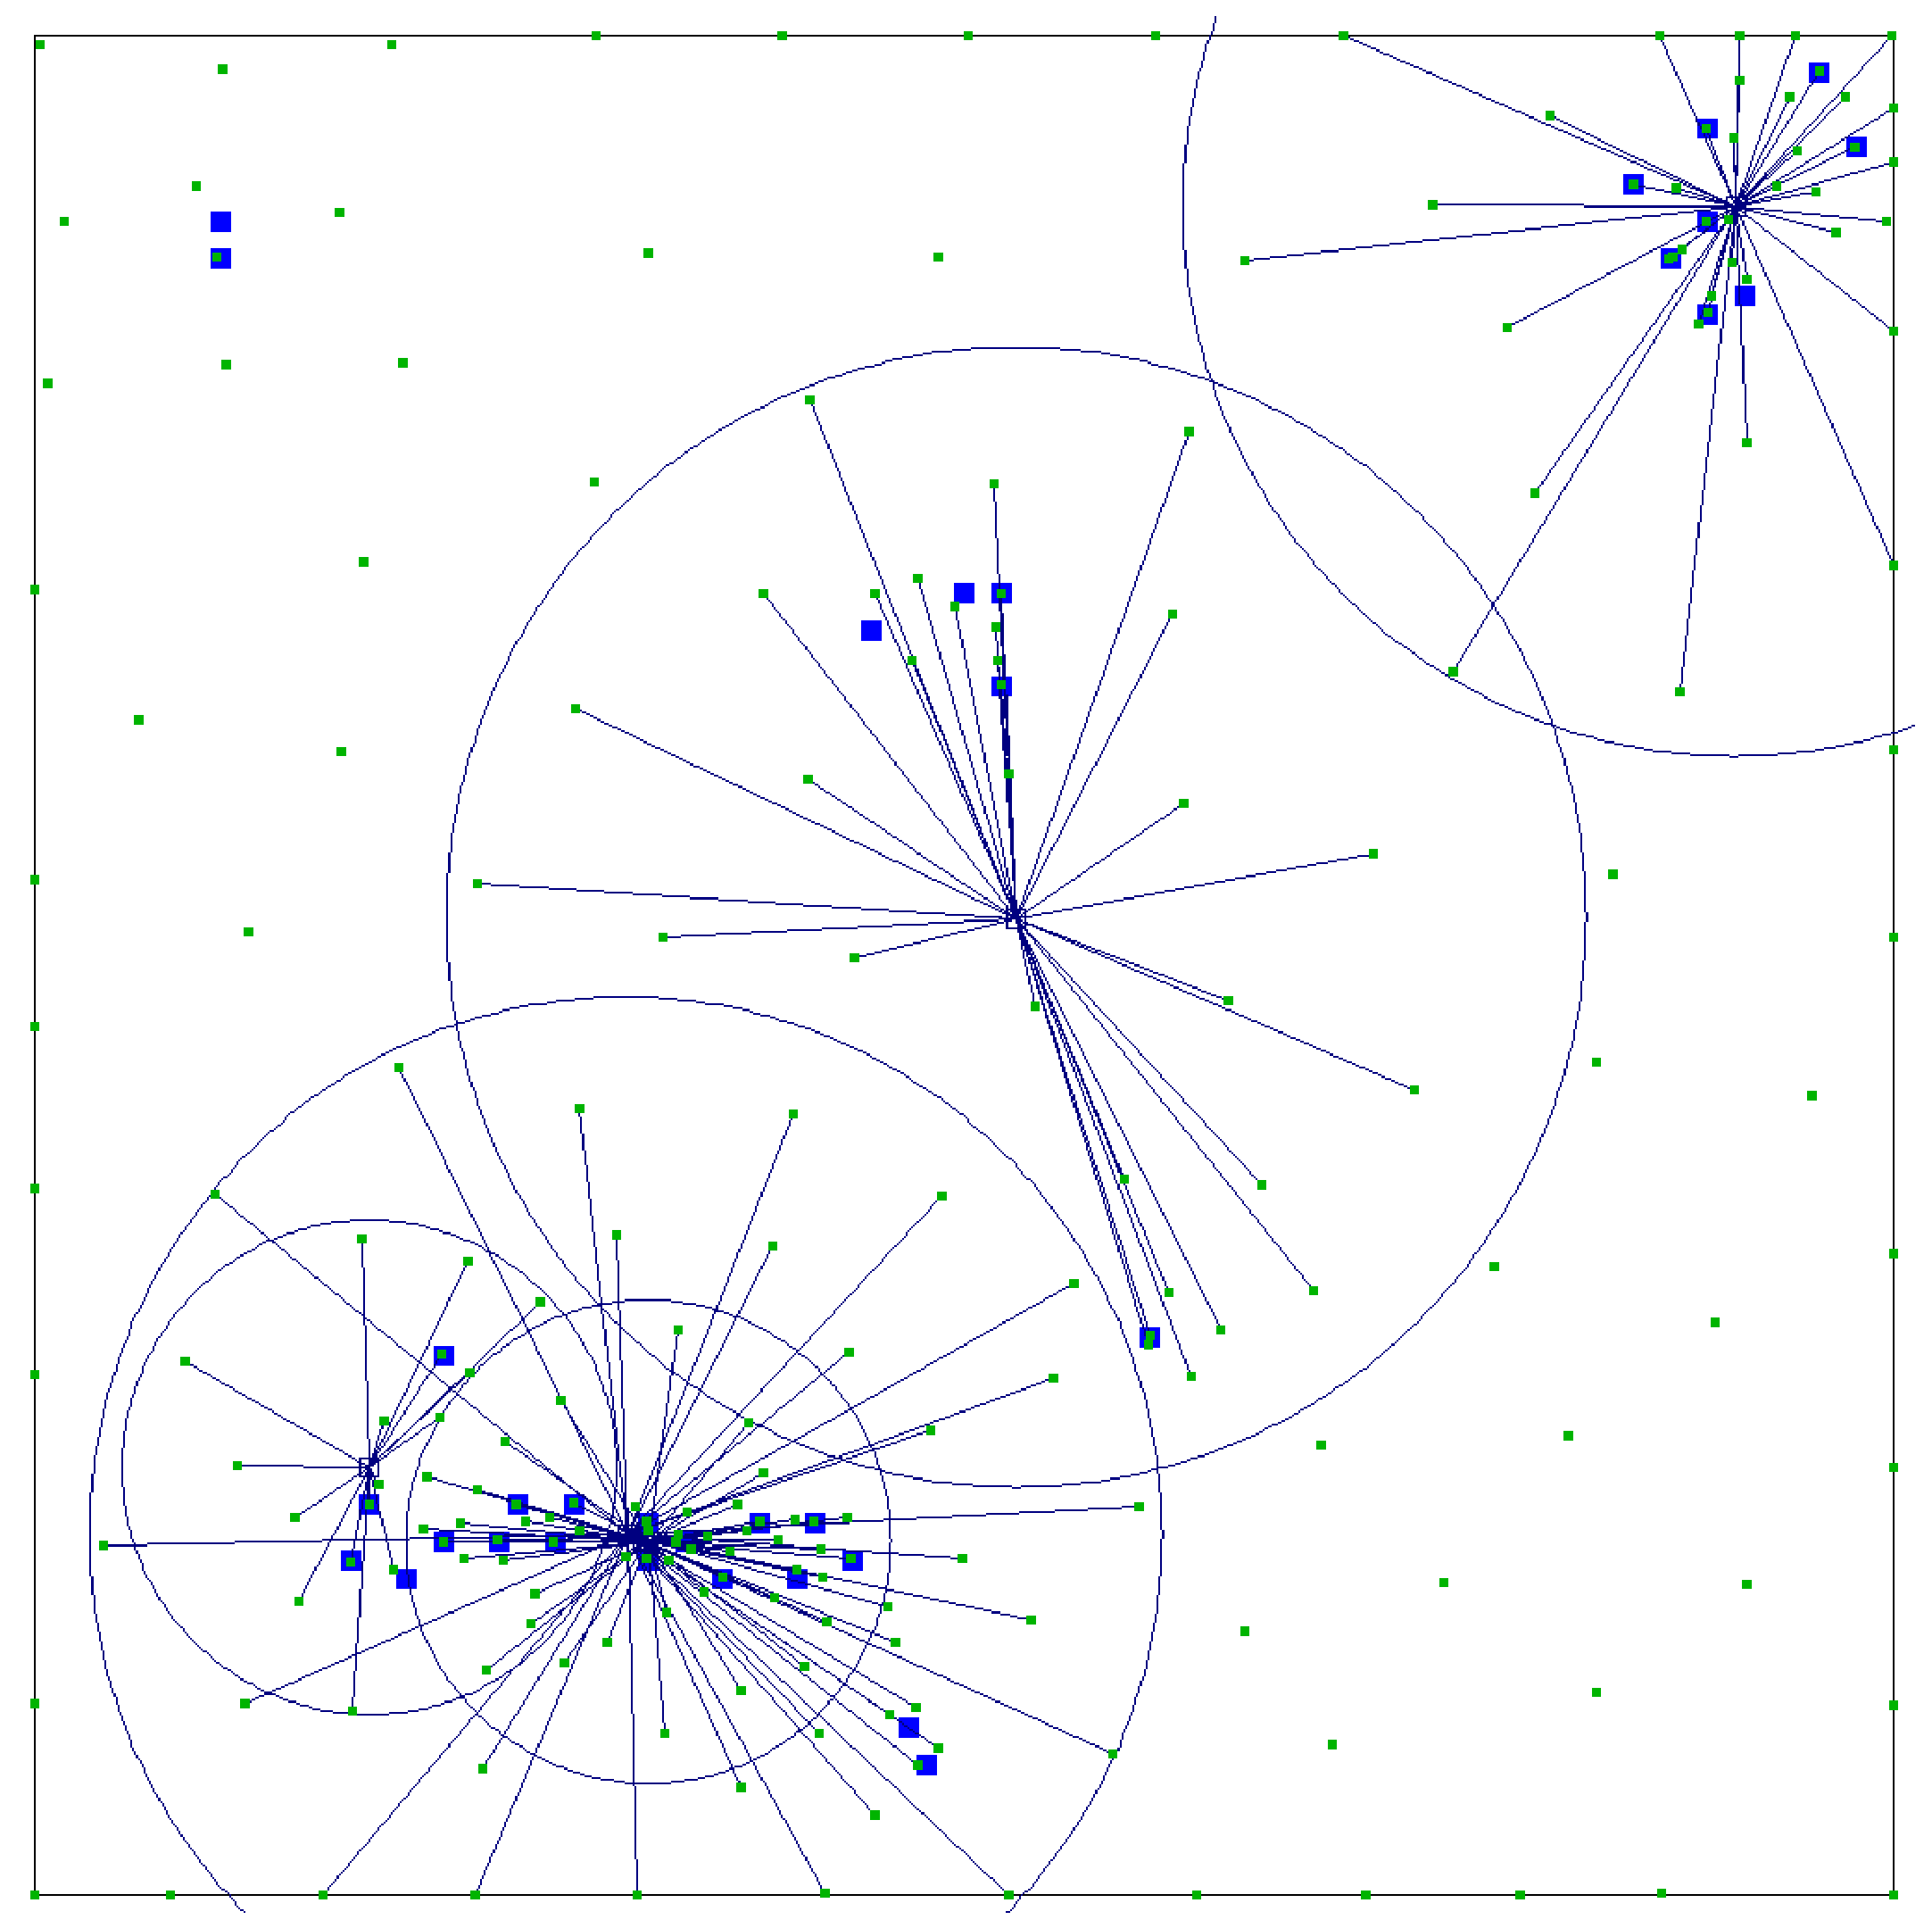
\includegraphics[width=0.5\textwidth]{img/final/heapline1000.eps}}
  \subfloat[Krok 5000]{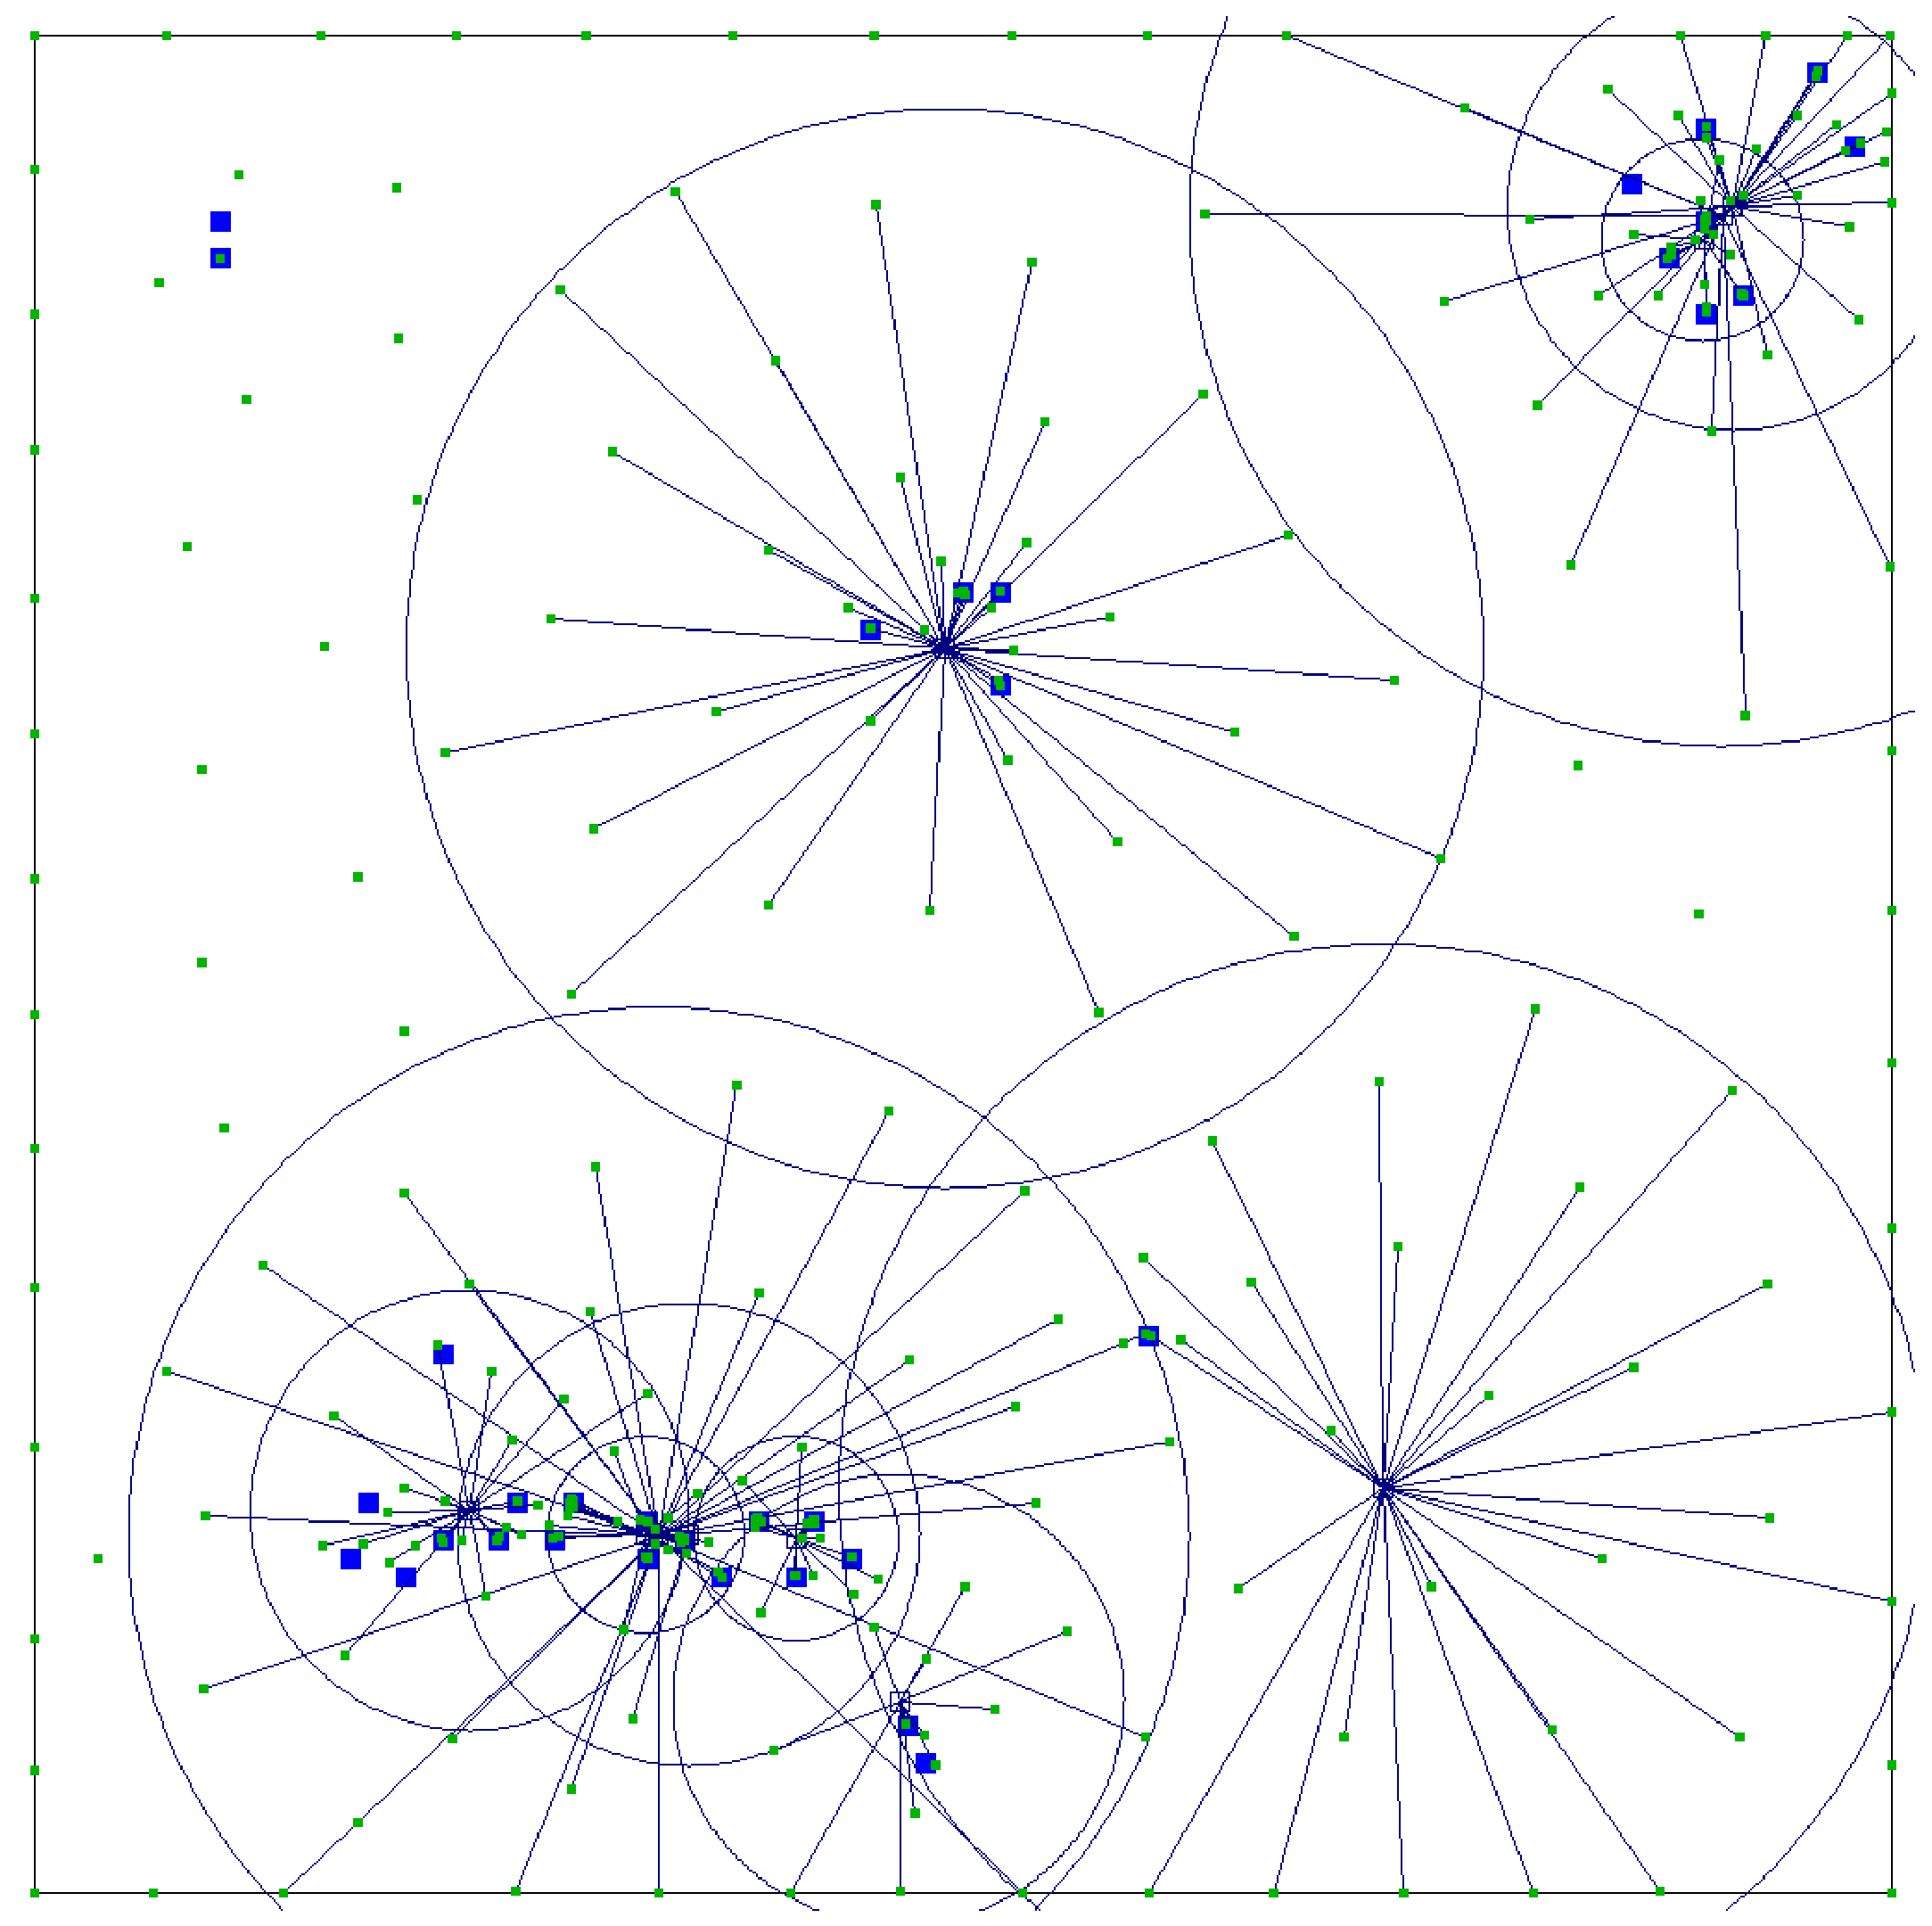
\includegraphics[width=0.5\textwidth]{img/final/heapline5000.eps}}
  \caption{Test v�sledn�ho modelu, m�stnost HeapLineRoom.}
  \label{fig:final-heapline}
\end{figure}


\newpage

\begin{figure}[h!]
  \centering
  \subfloat[Krok 1000]{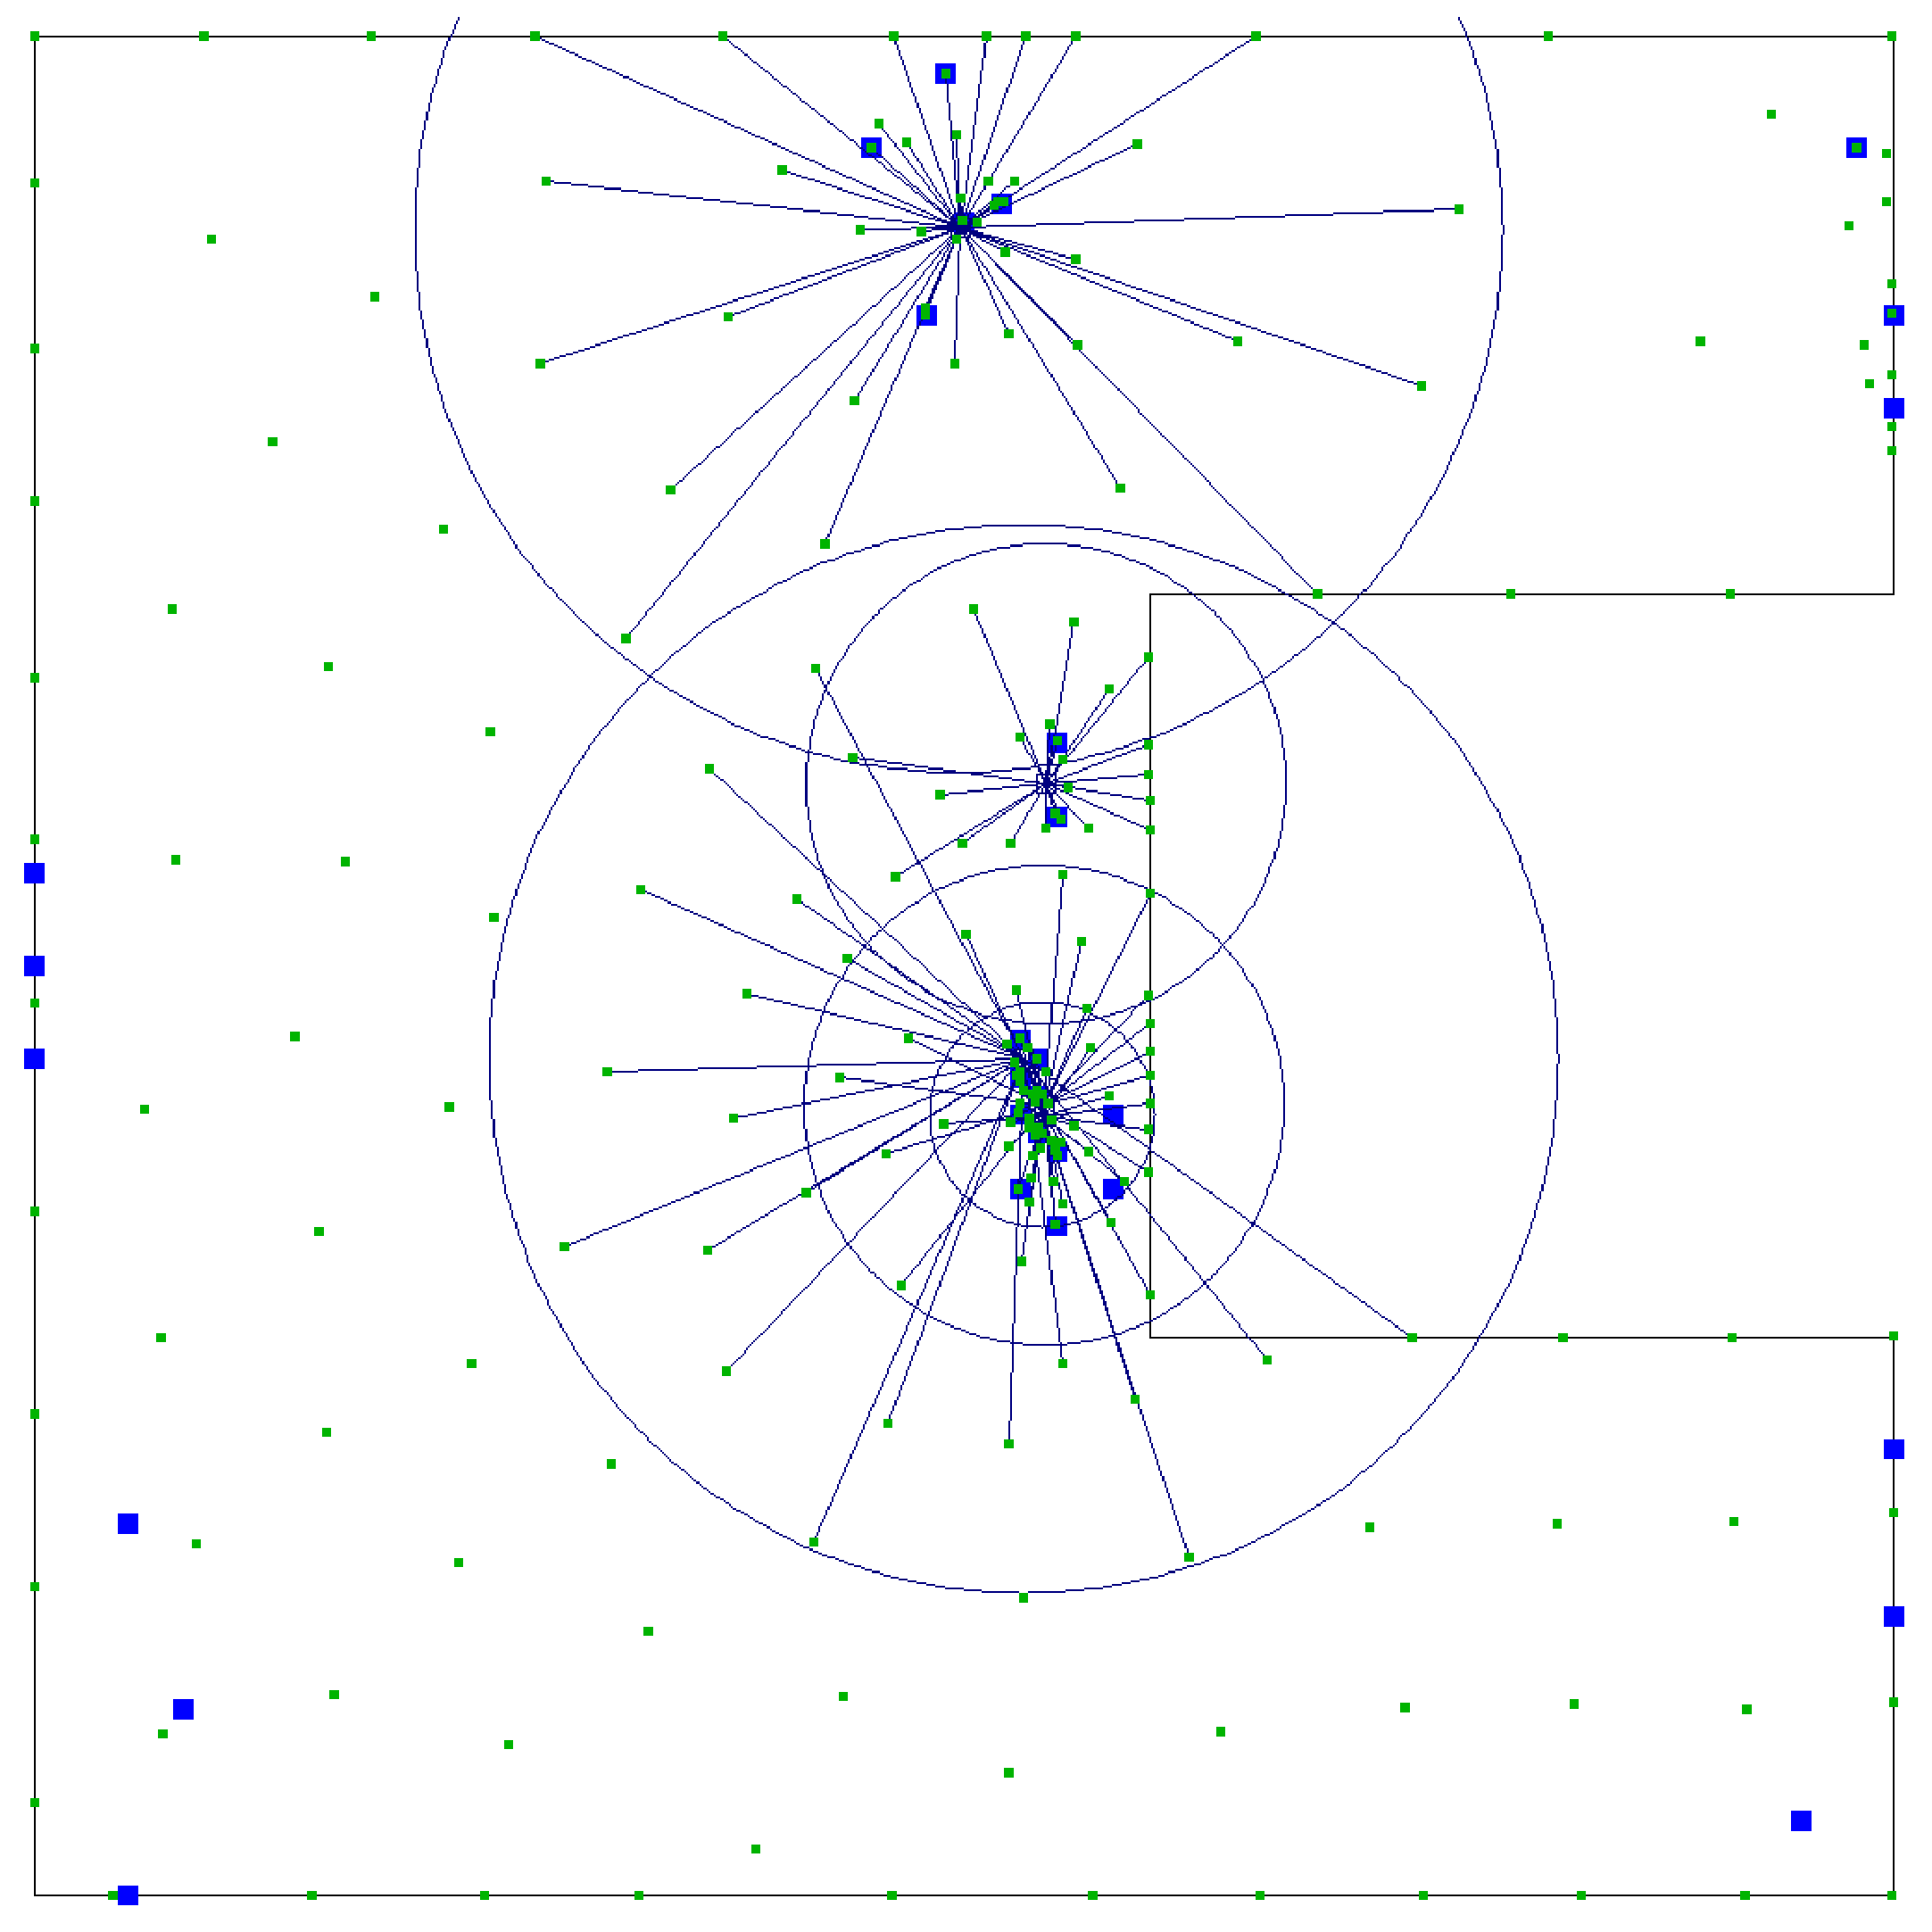
\includegraphics[width=0.5\textwidth]{img/final/lobby1000.eps}}
  \subfloat[Krok 5000]{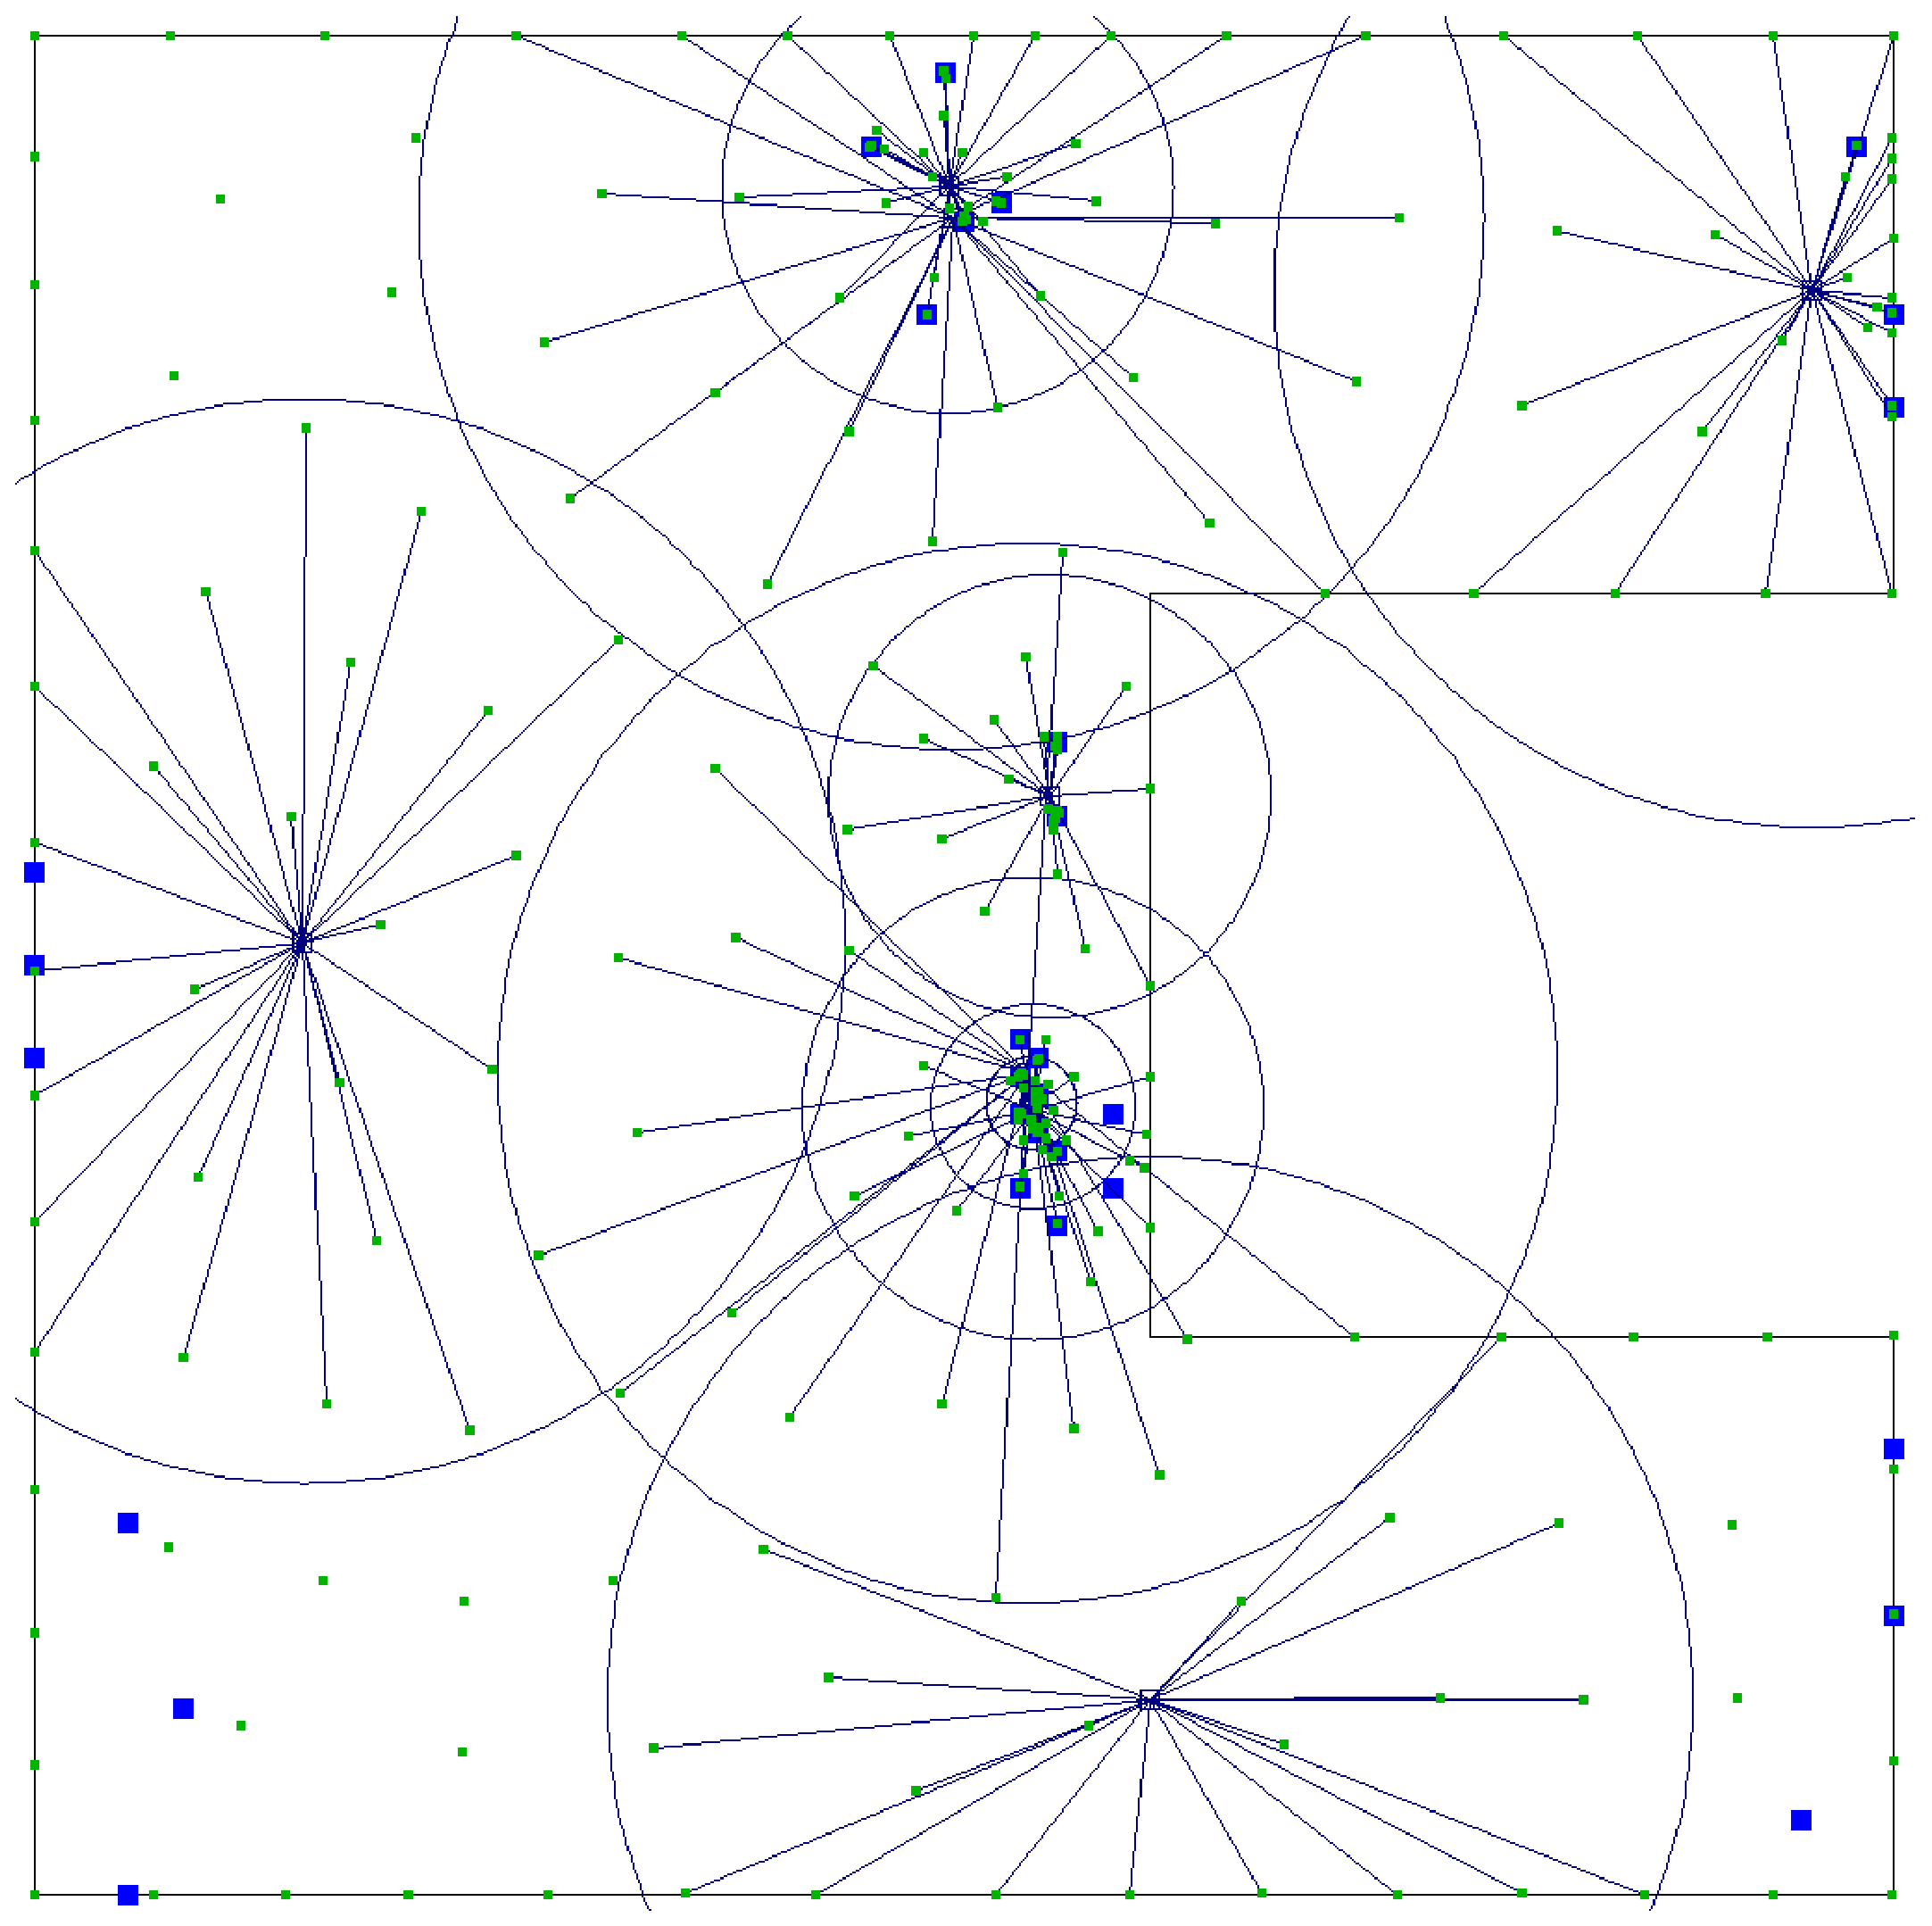
\includegraphics[width=0.5\textwidth]{img/final/lobby5000.eps}}
  \caption{Test v�sledn�ho modelu, m�stnost Lobby.}
  \label{fig:final-lobby}
\end{figure}





\section{Vliv napln�nosti} \label{chapter-test-ag}

V tomto testu uk�eme, jak d�le�itou roli hraje vliv napln�nosti p�i ur�ov�n� vz�jemn� odpudivosti dvou uzl� ve vzorci \eqref{formula:el-odpudivost}.
Provedli jsme 5000 krok� simulace v m�stnostech EmptyRoom a FullRoom.
\\

V prvn�m testu nebyla napln�nost uzl� p�i po��t�n� odpudivosti v�bec br�na v �vahu.
V�sledek je na obr�zku \ref{fig:usage-ag-no} a ukazuje, �e v tomto p��pad� model rozmis�uje uzly v prostoru t�m�� rovnom�rn�.
Z toho vypl�v�, �e napln�nost uzlu hraje v modelu v�znamnou roli.
Obr�zky \ref{fig:usage-ag-0.5}, \ref{fig:usage-ag-0.8}, \ref{fig:usage-ag-1} ukazuj� v�sledky test� pro r�zn� hodnoty parametru \param{vliv napln�nosti}.
\\

\begin{figure}[p]
  \centering
  \subfloat[EmptyRoom]{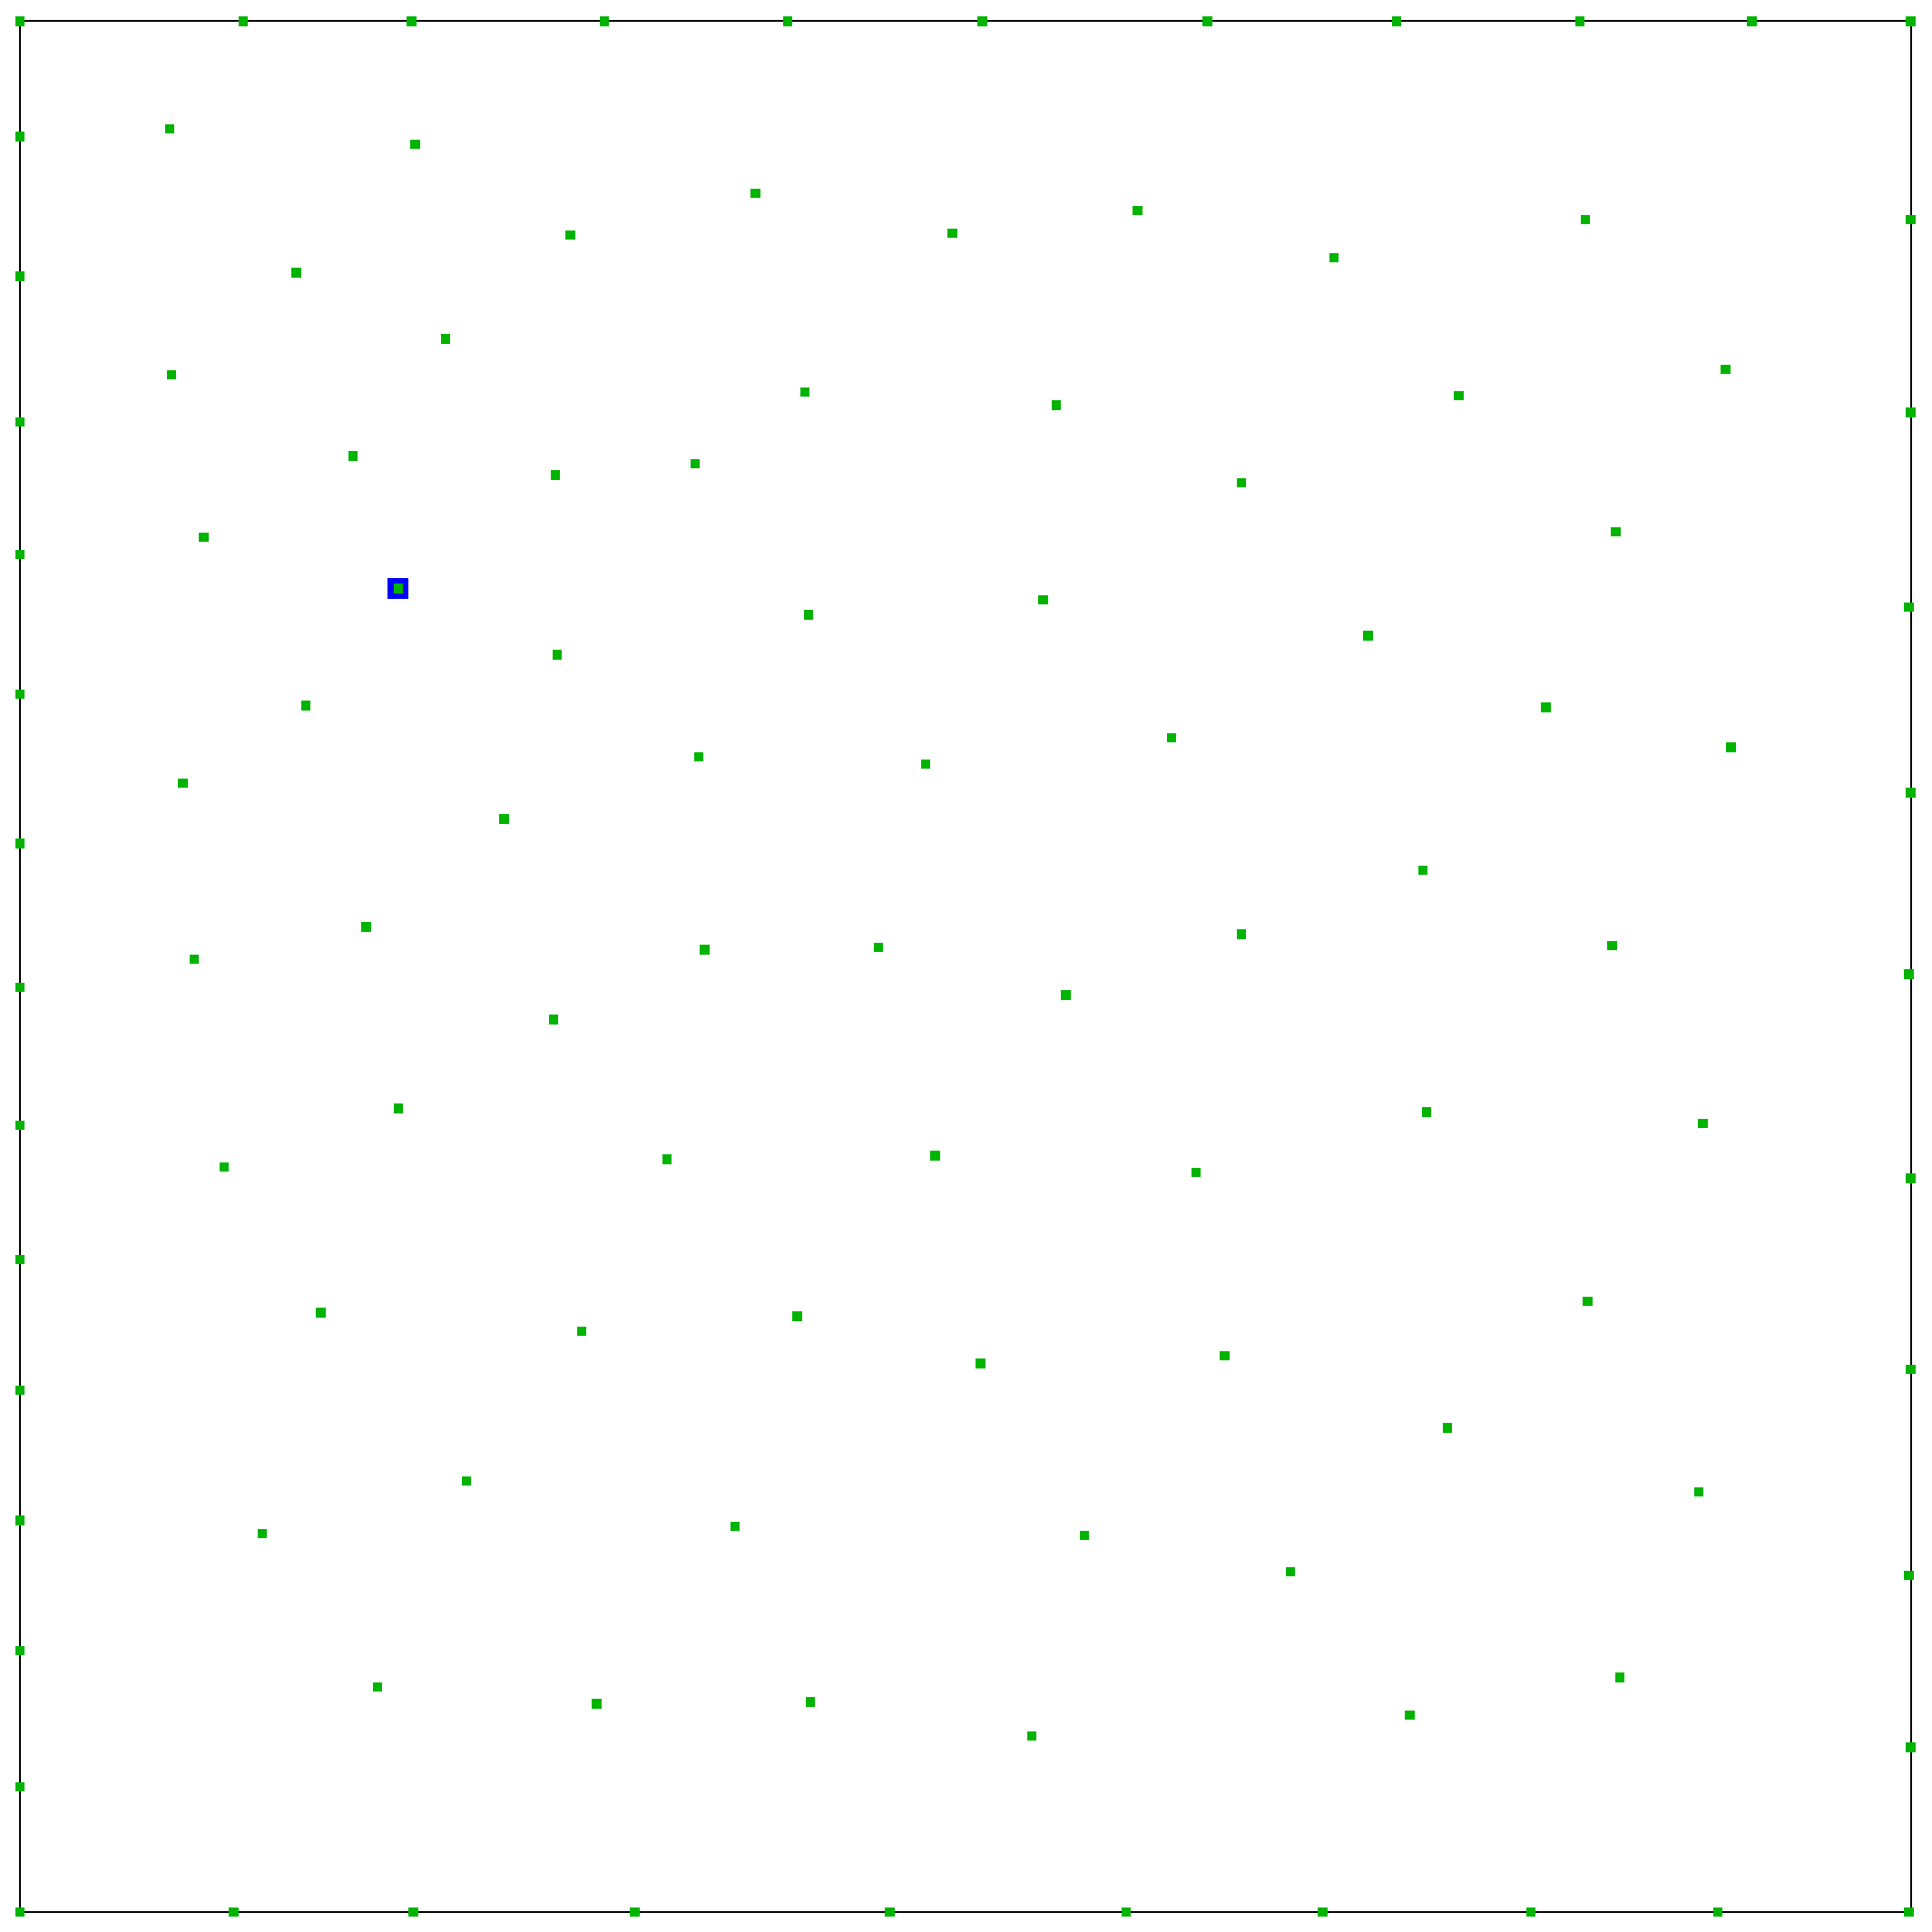
\includegraphics[width=0.5\textwidth]{img/usage/nousage-empty.eps}}
  \subfloat[FullRoom]{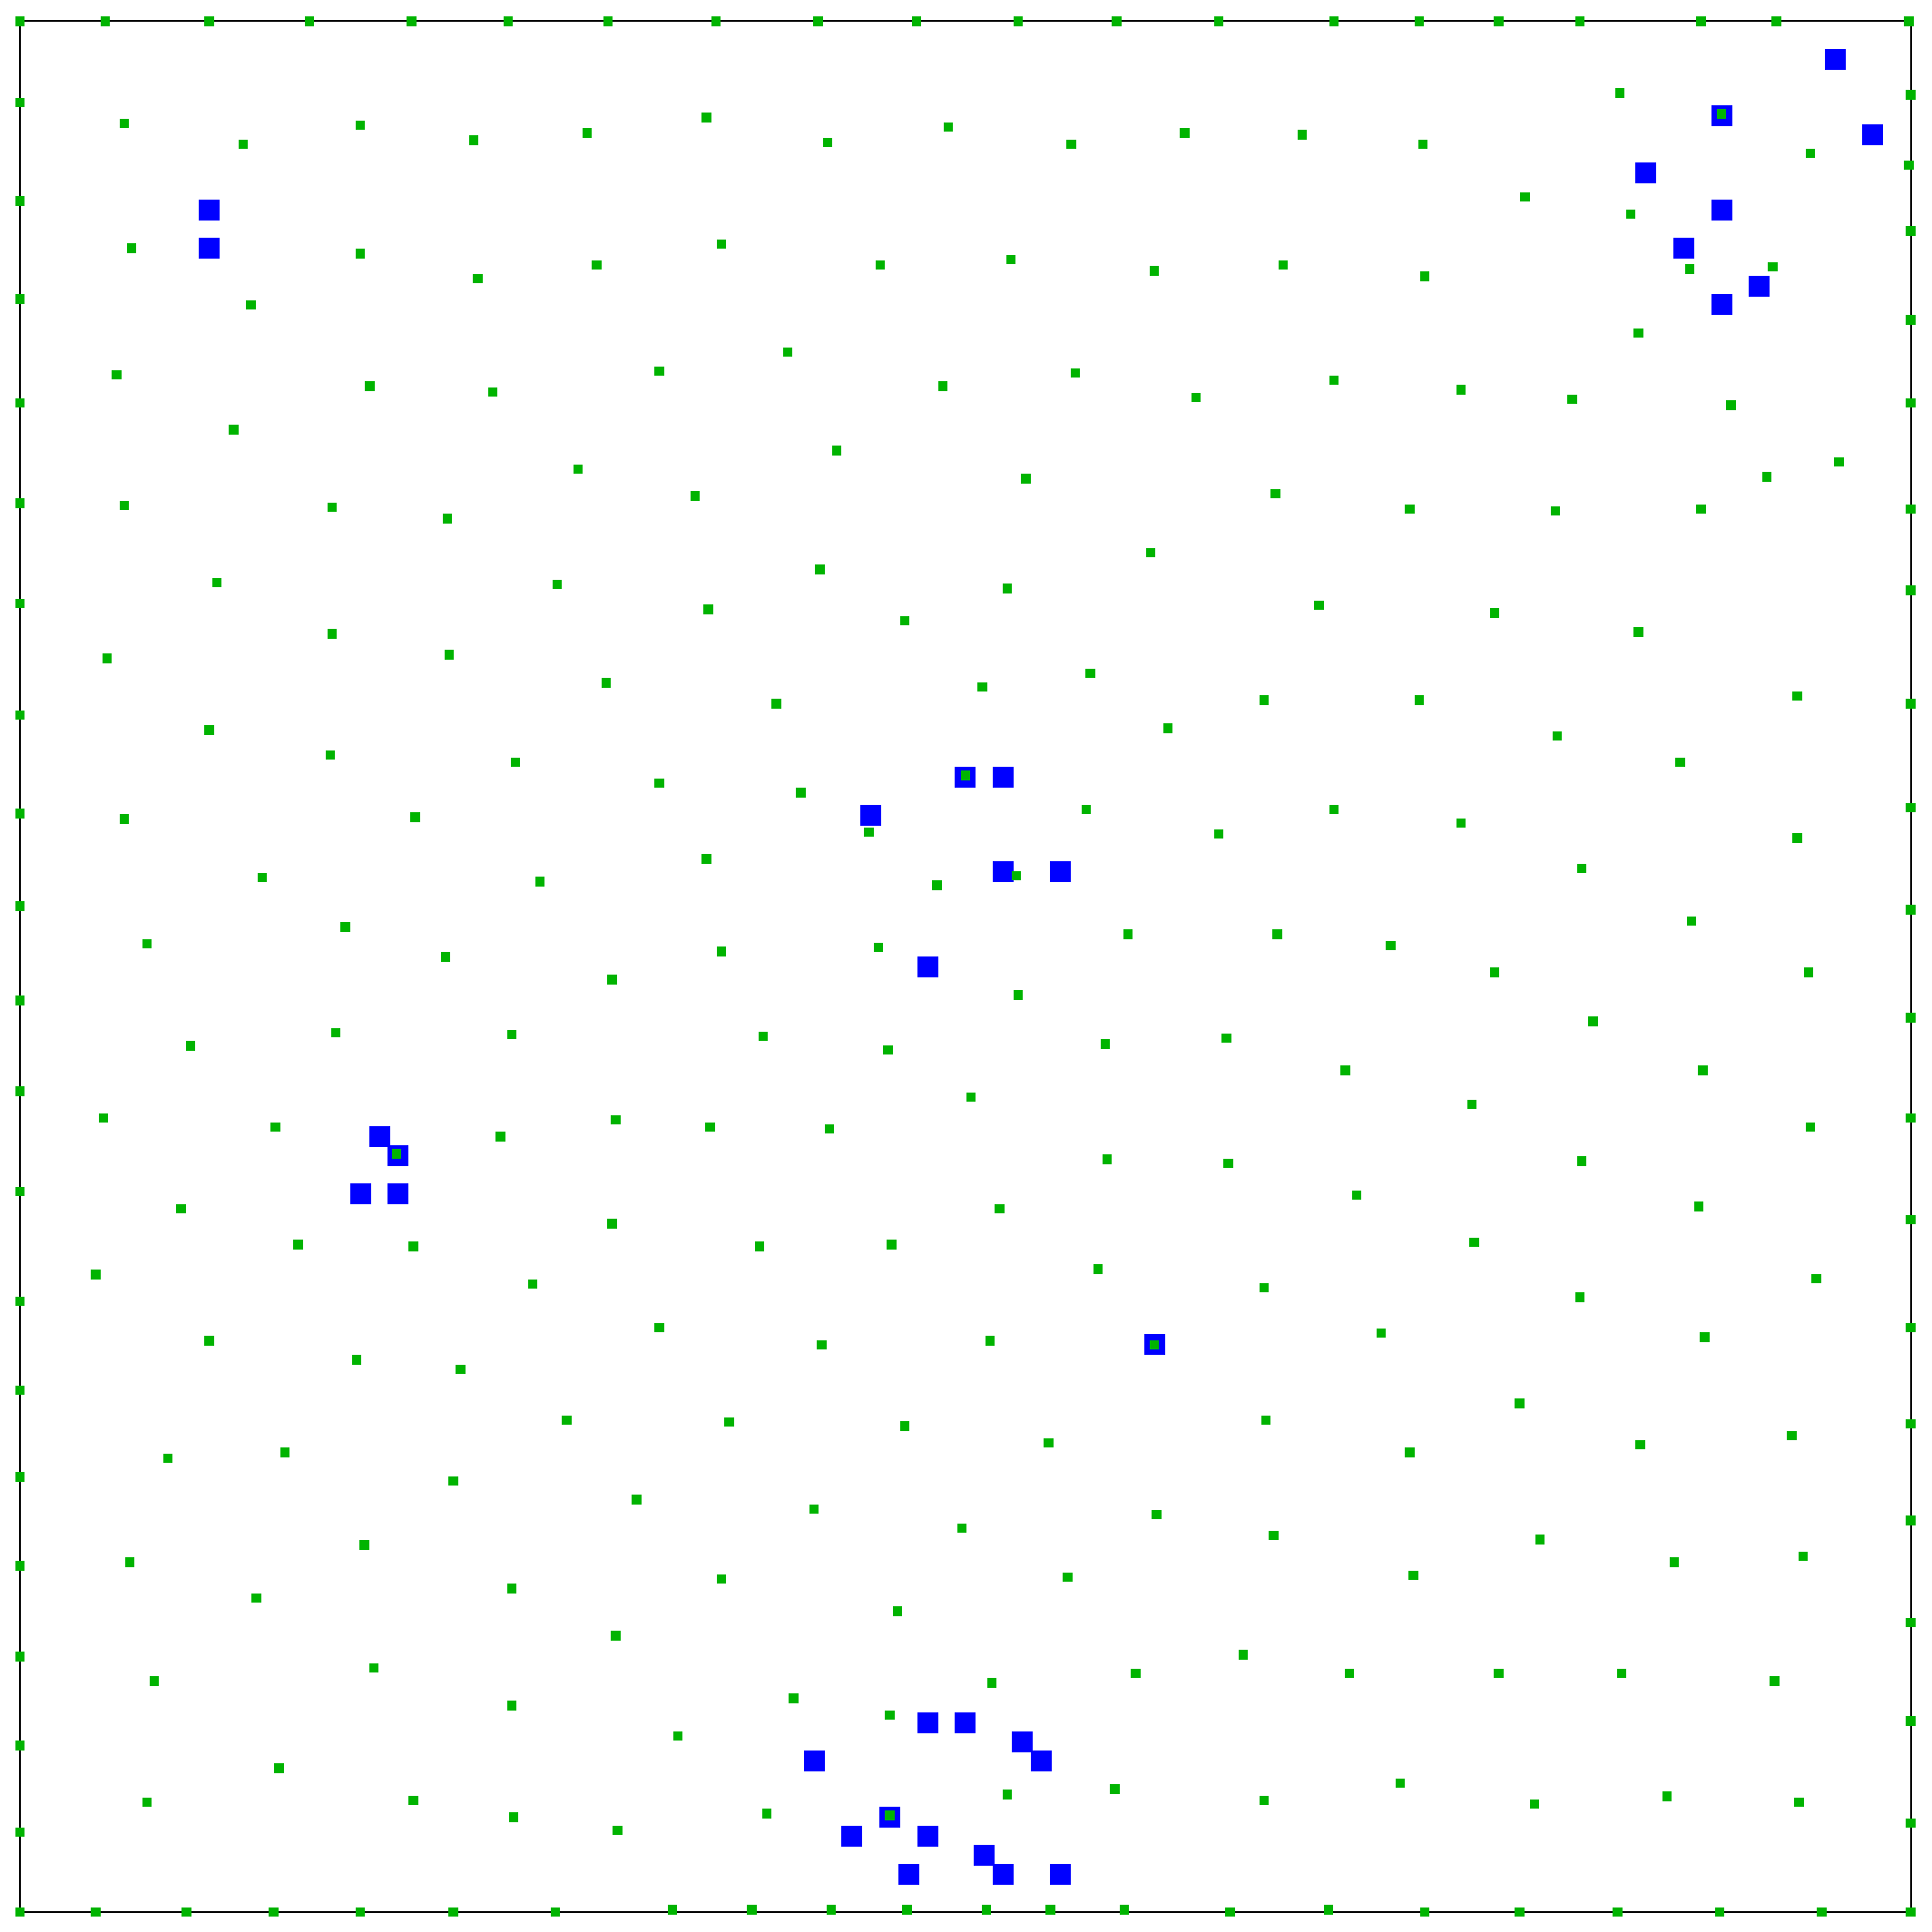
\includegraphics[width=0.5\textwidth]{img/usage/nousage-full.eps}}
  \caption{Test odpudivosti uzl�, jejich napln�nost nen� br�na v uvahu.}
  \label{fig:usage-ag-no}
\end{figure}

\begin{figure}[p]
  \centering
  \subfloat[EmptyRoom]{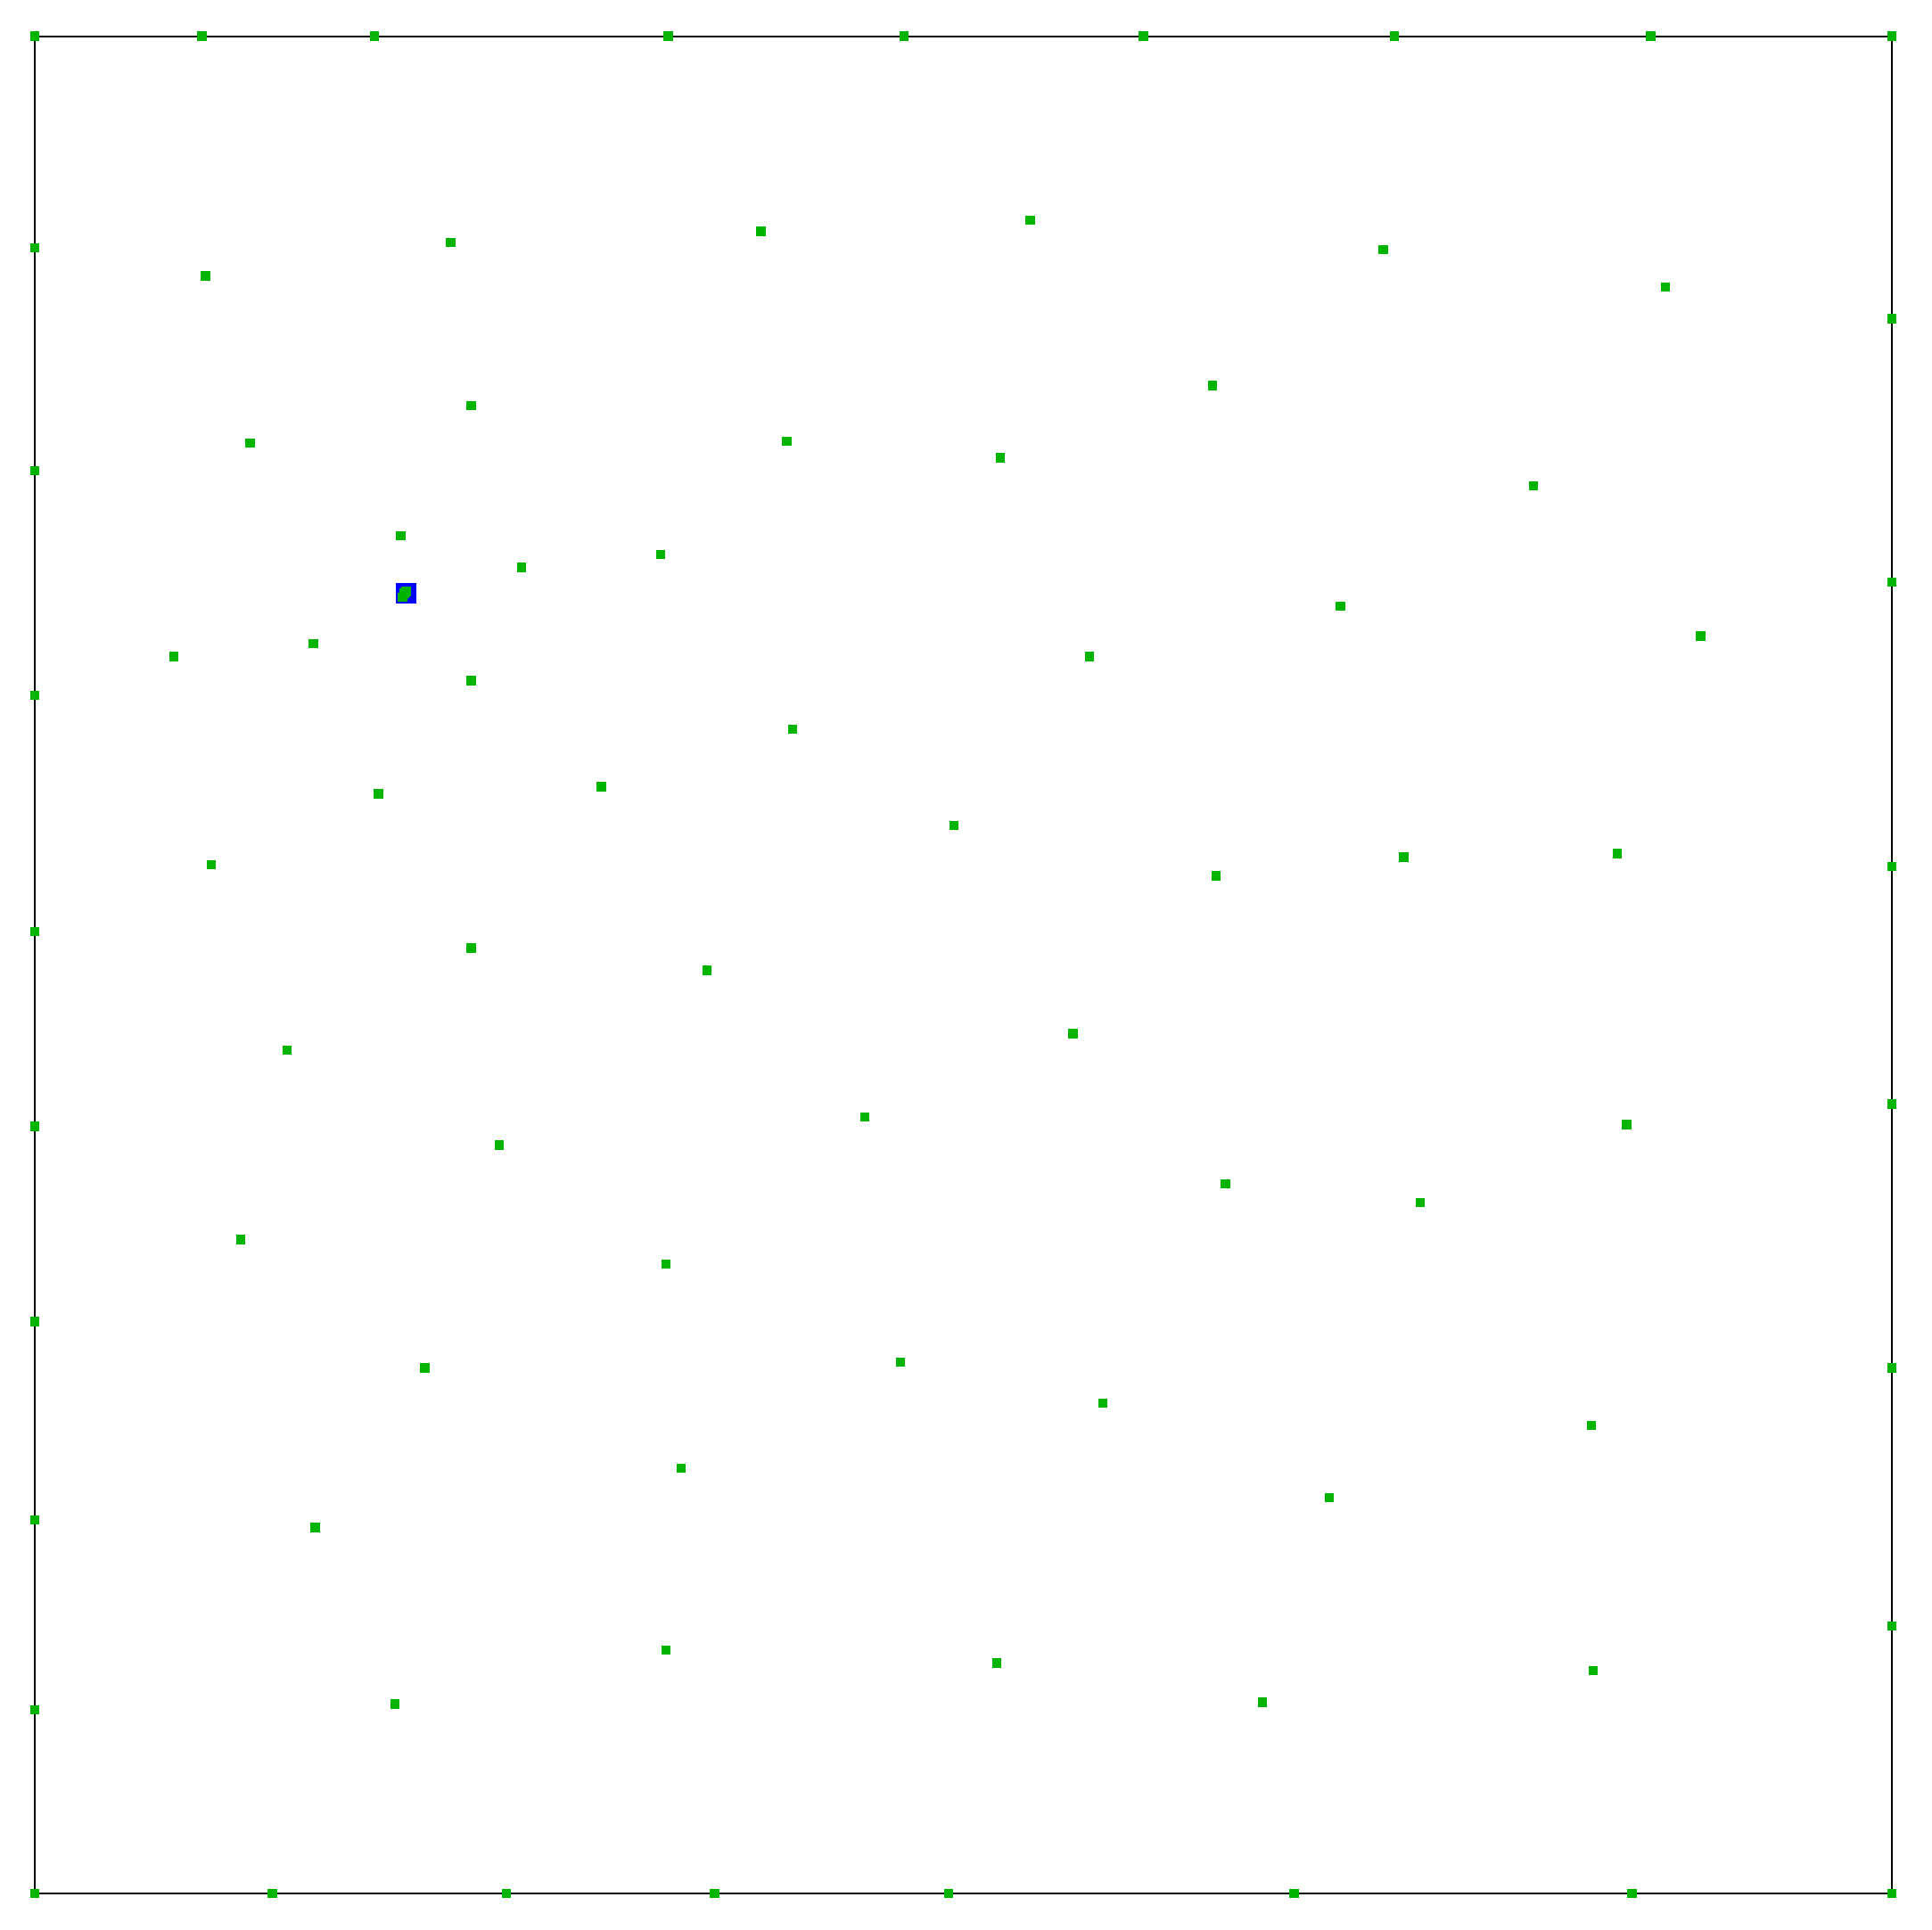
\includegraphics[width=0.5\textwidth]{img/usage/usage1-empty.eps}}
  \subfloat[FullRoom]{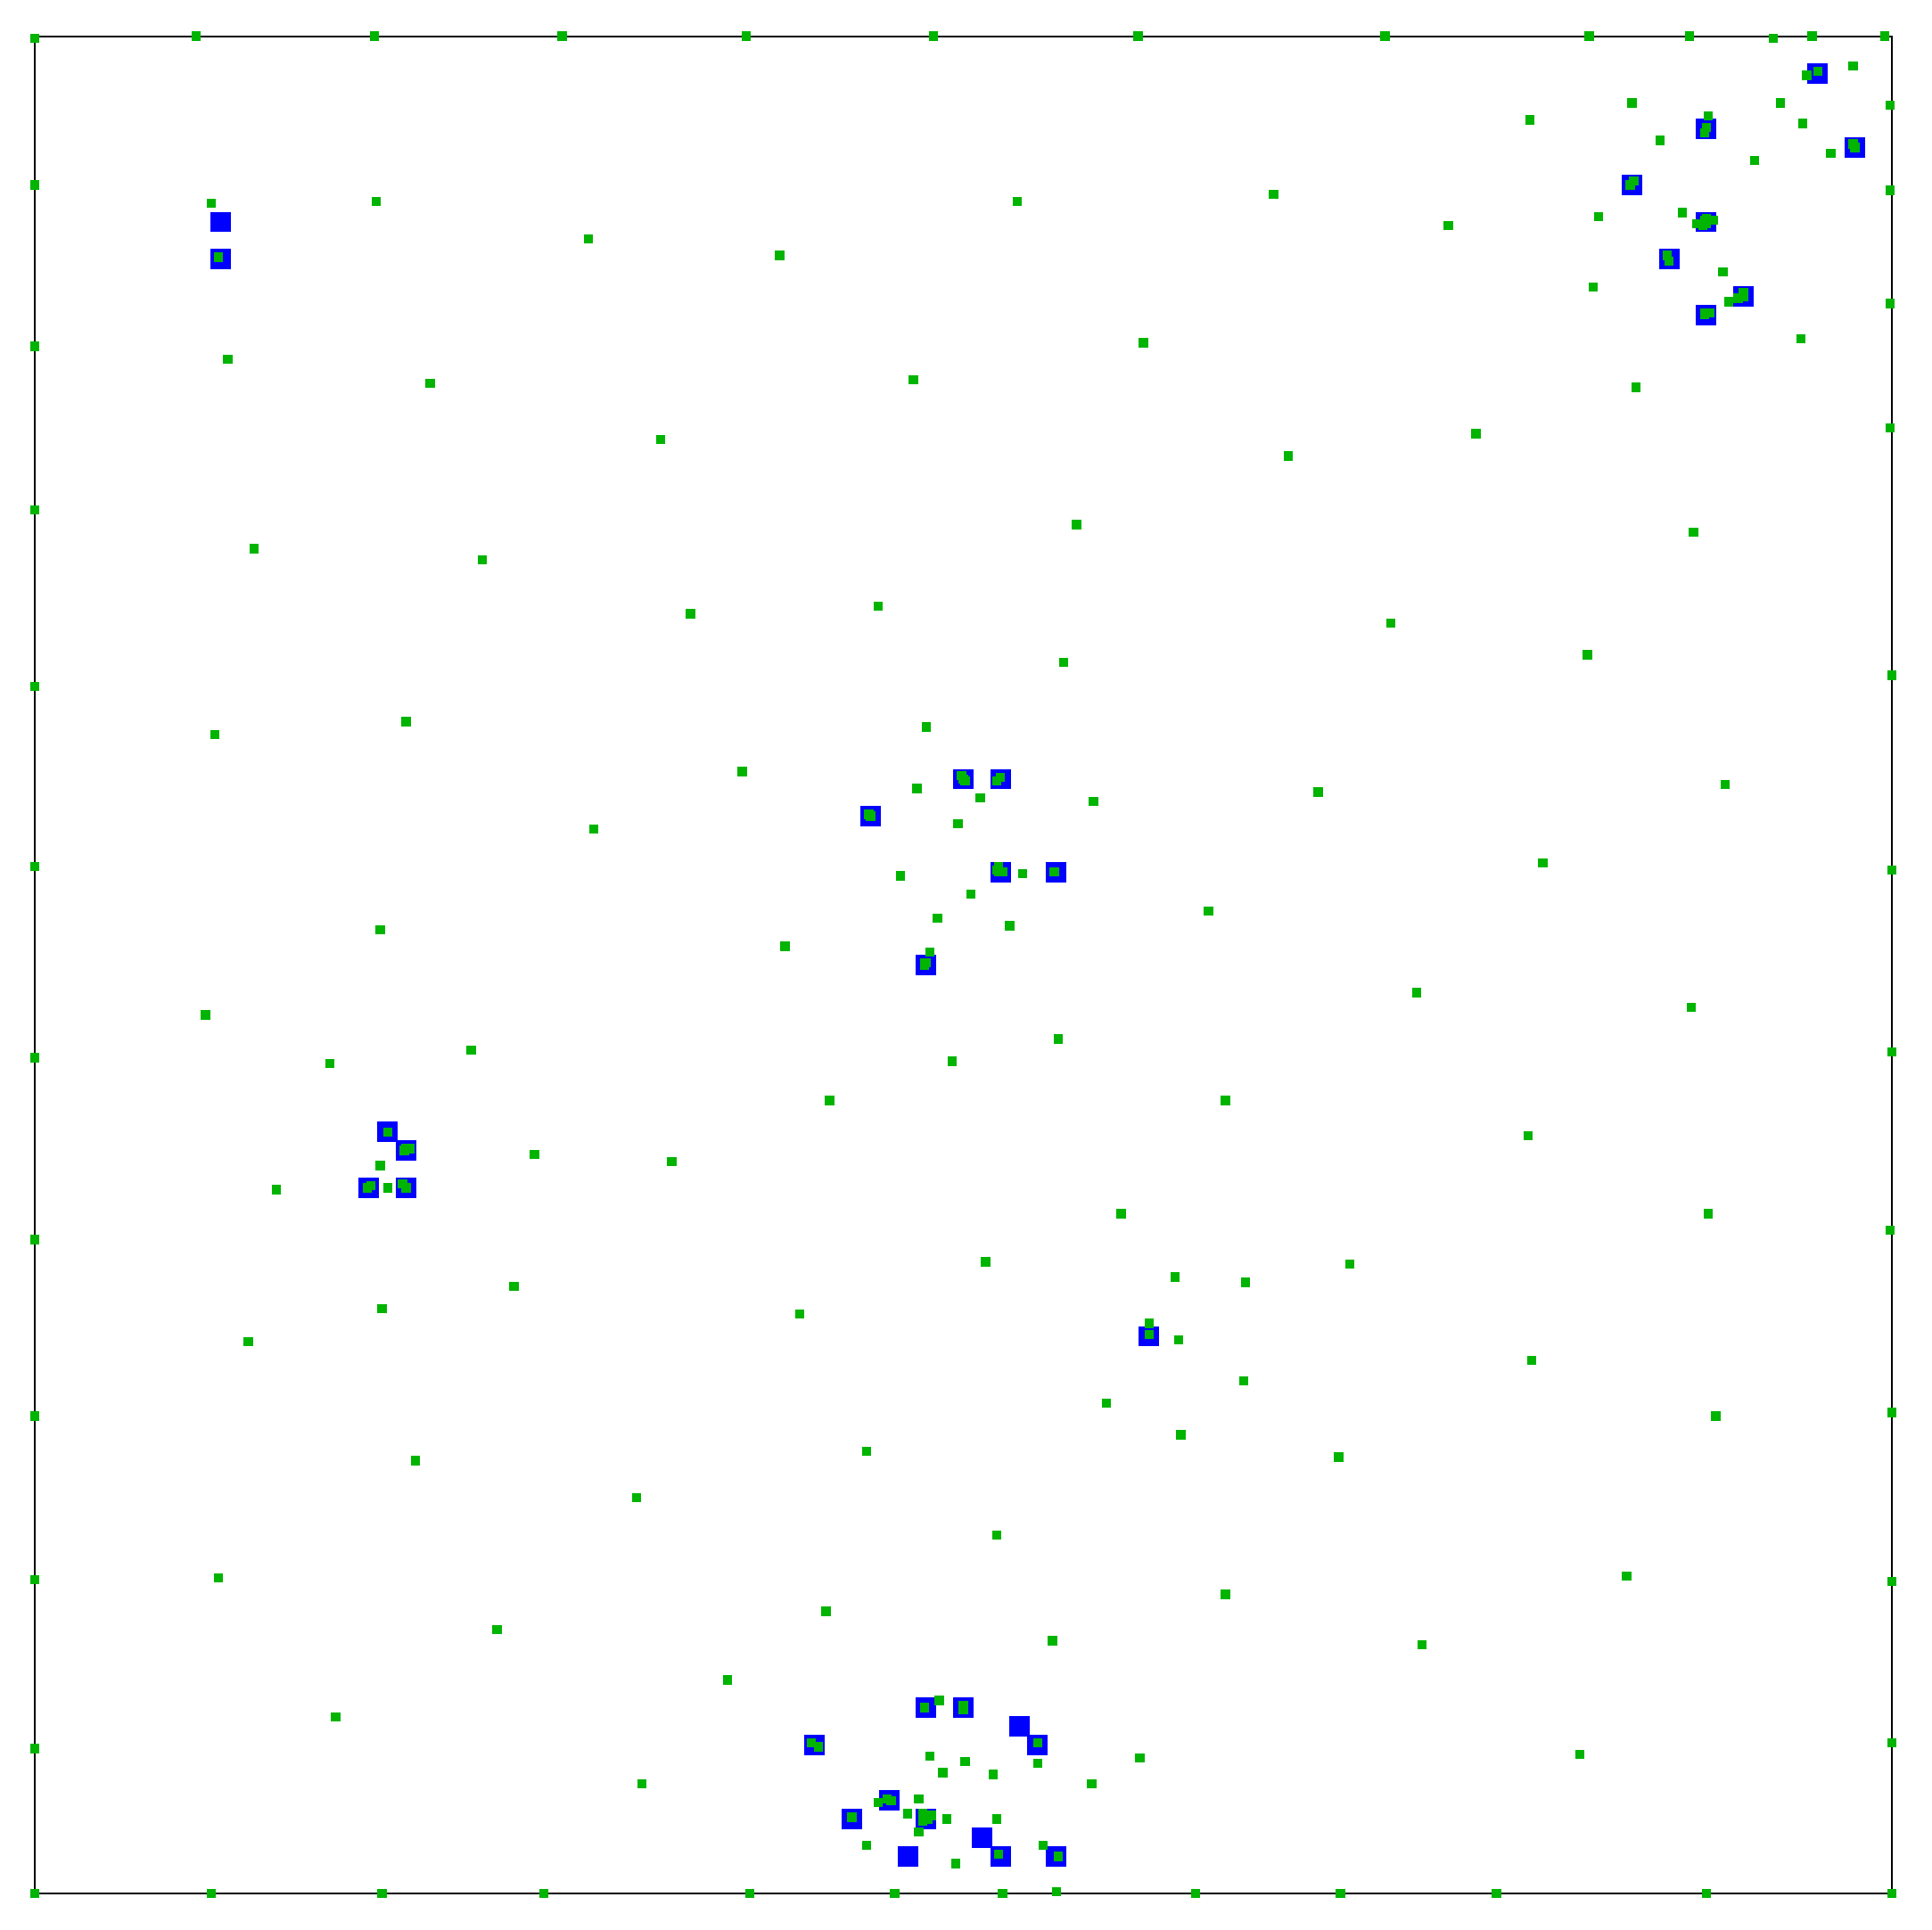
\includegraphics[width=0.5\textwidth]{img/usage/usage1-full.eps}}
  \caption{Test odpudivosti uzl�, vliv napln�nosti $=1$.}
  \label{fig:usage-ag-1}
\end{figure}

\begin{figure}[p]
  \centering
  \subfloat[EmptyRoom]{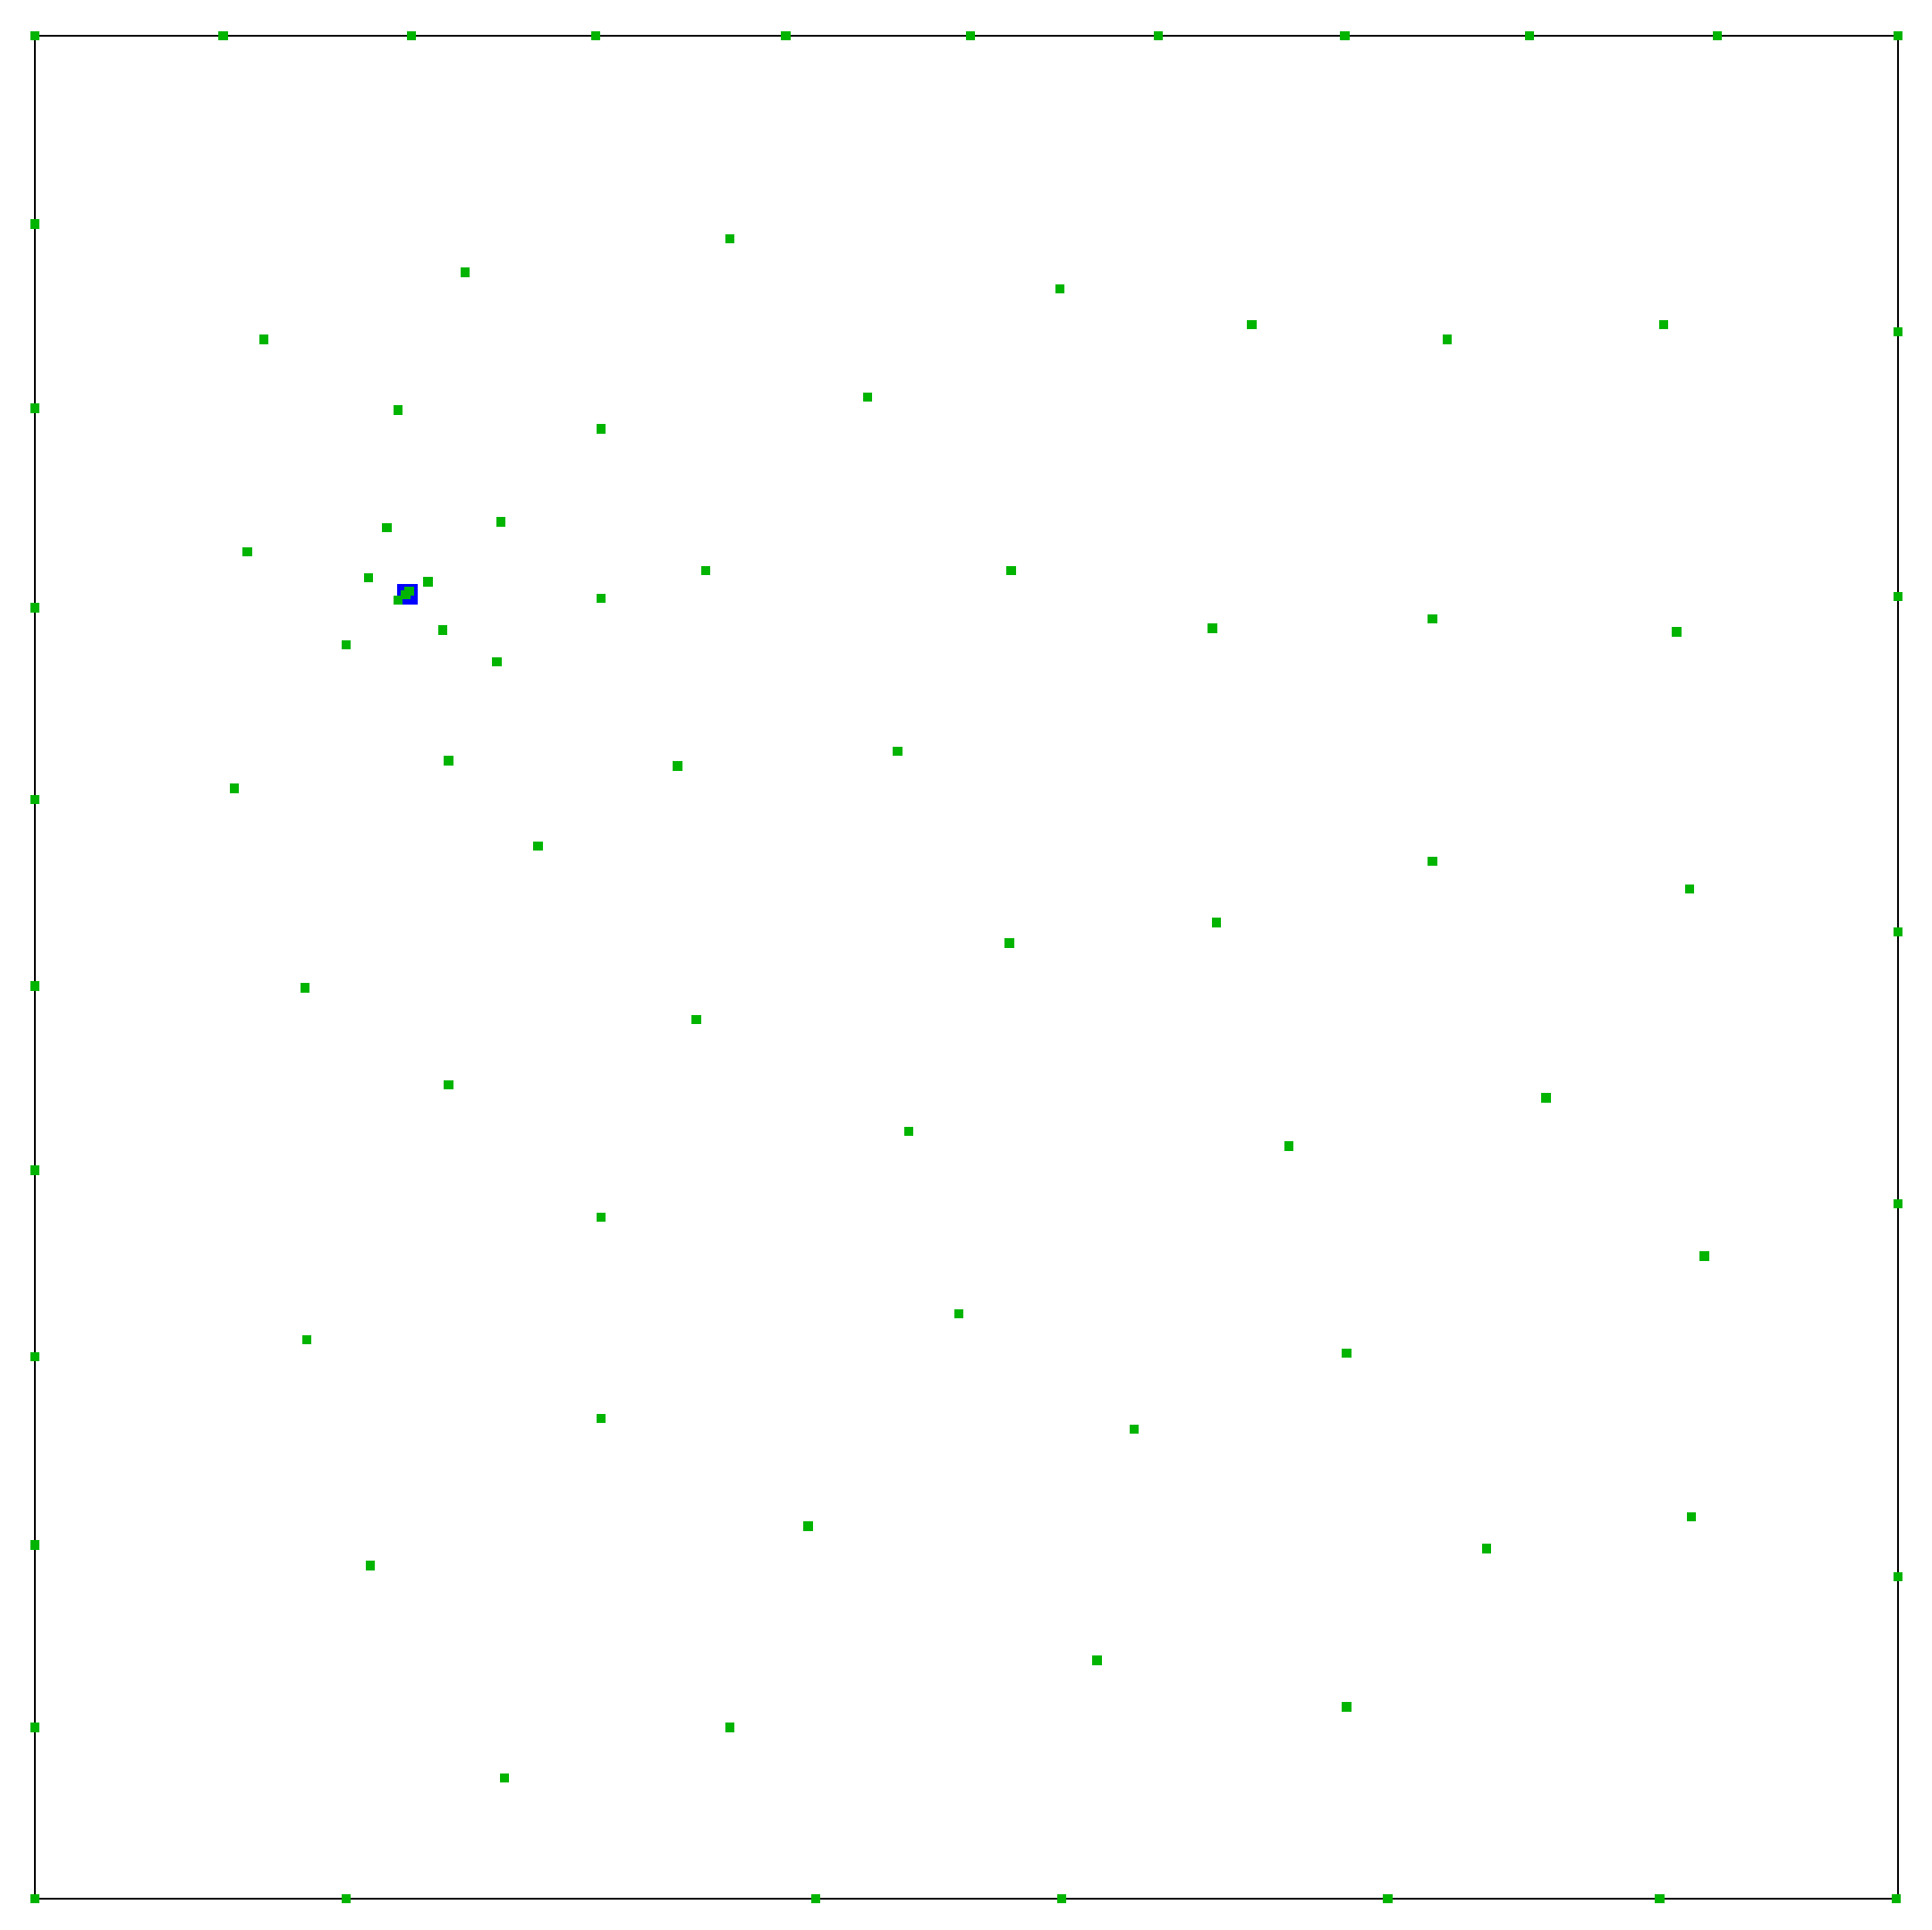
\includegraphics[width=0.5\textwidth]{img/usage/usage0.8-empty.eps}}
  \subfloat[FullRoom]{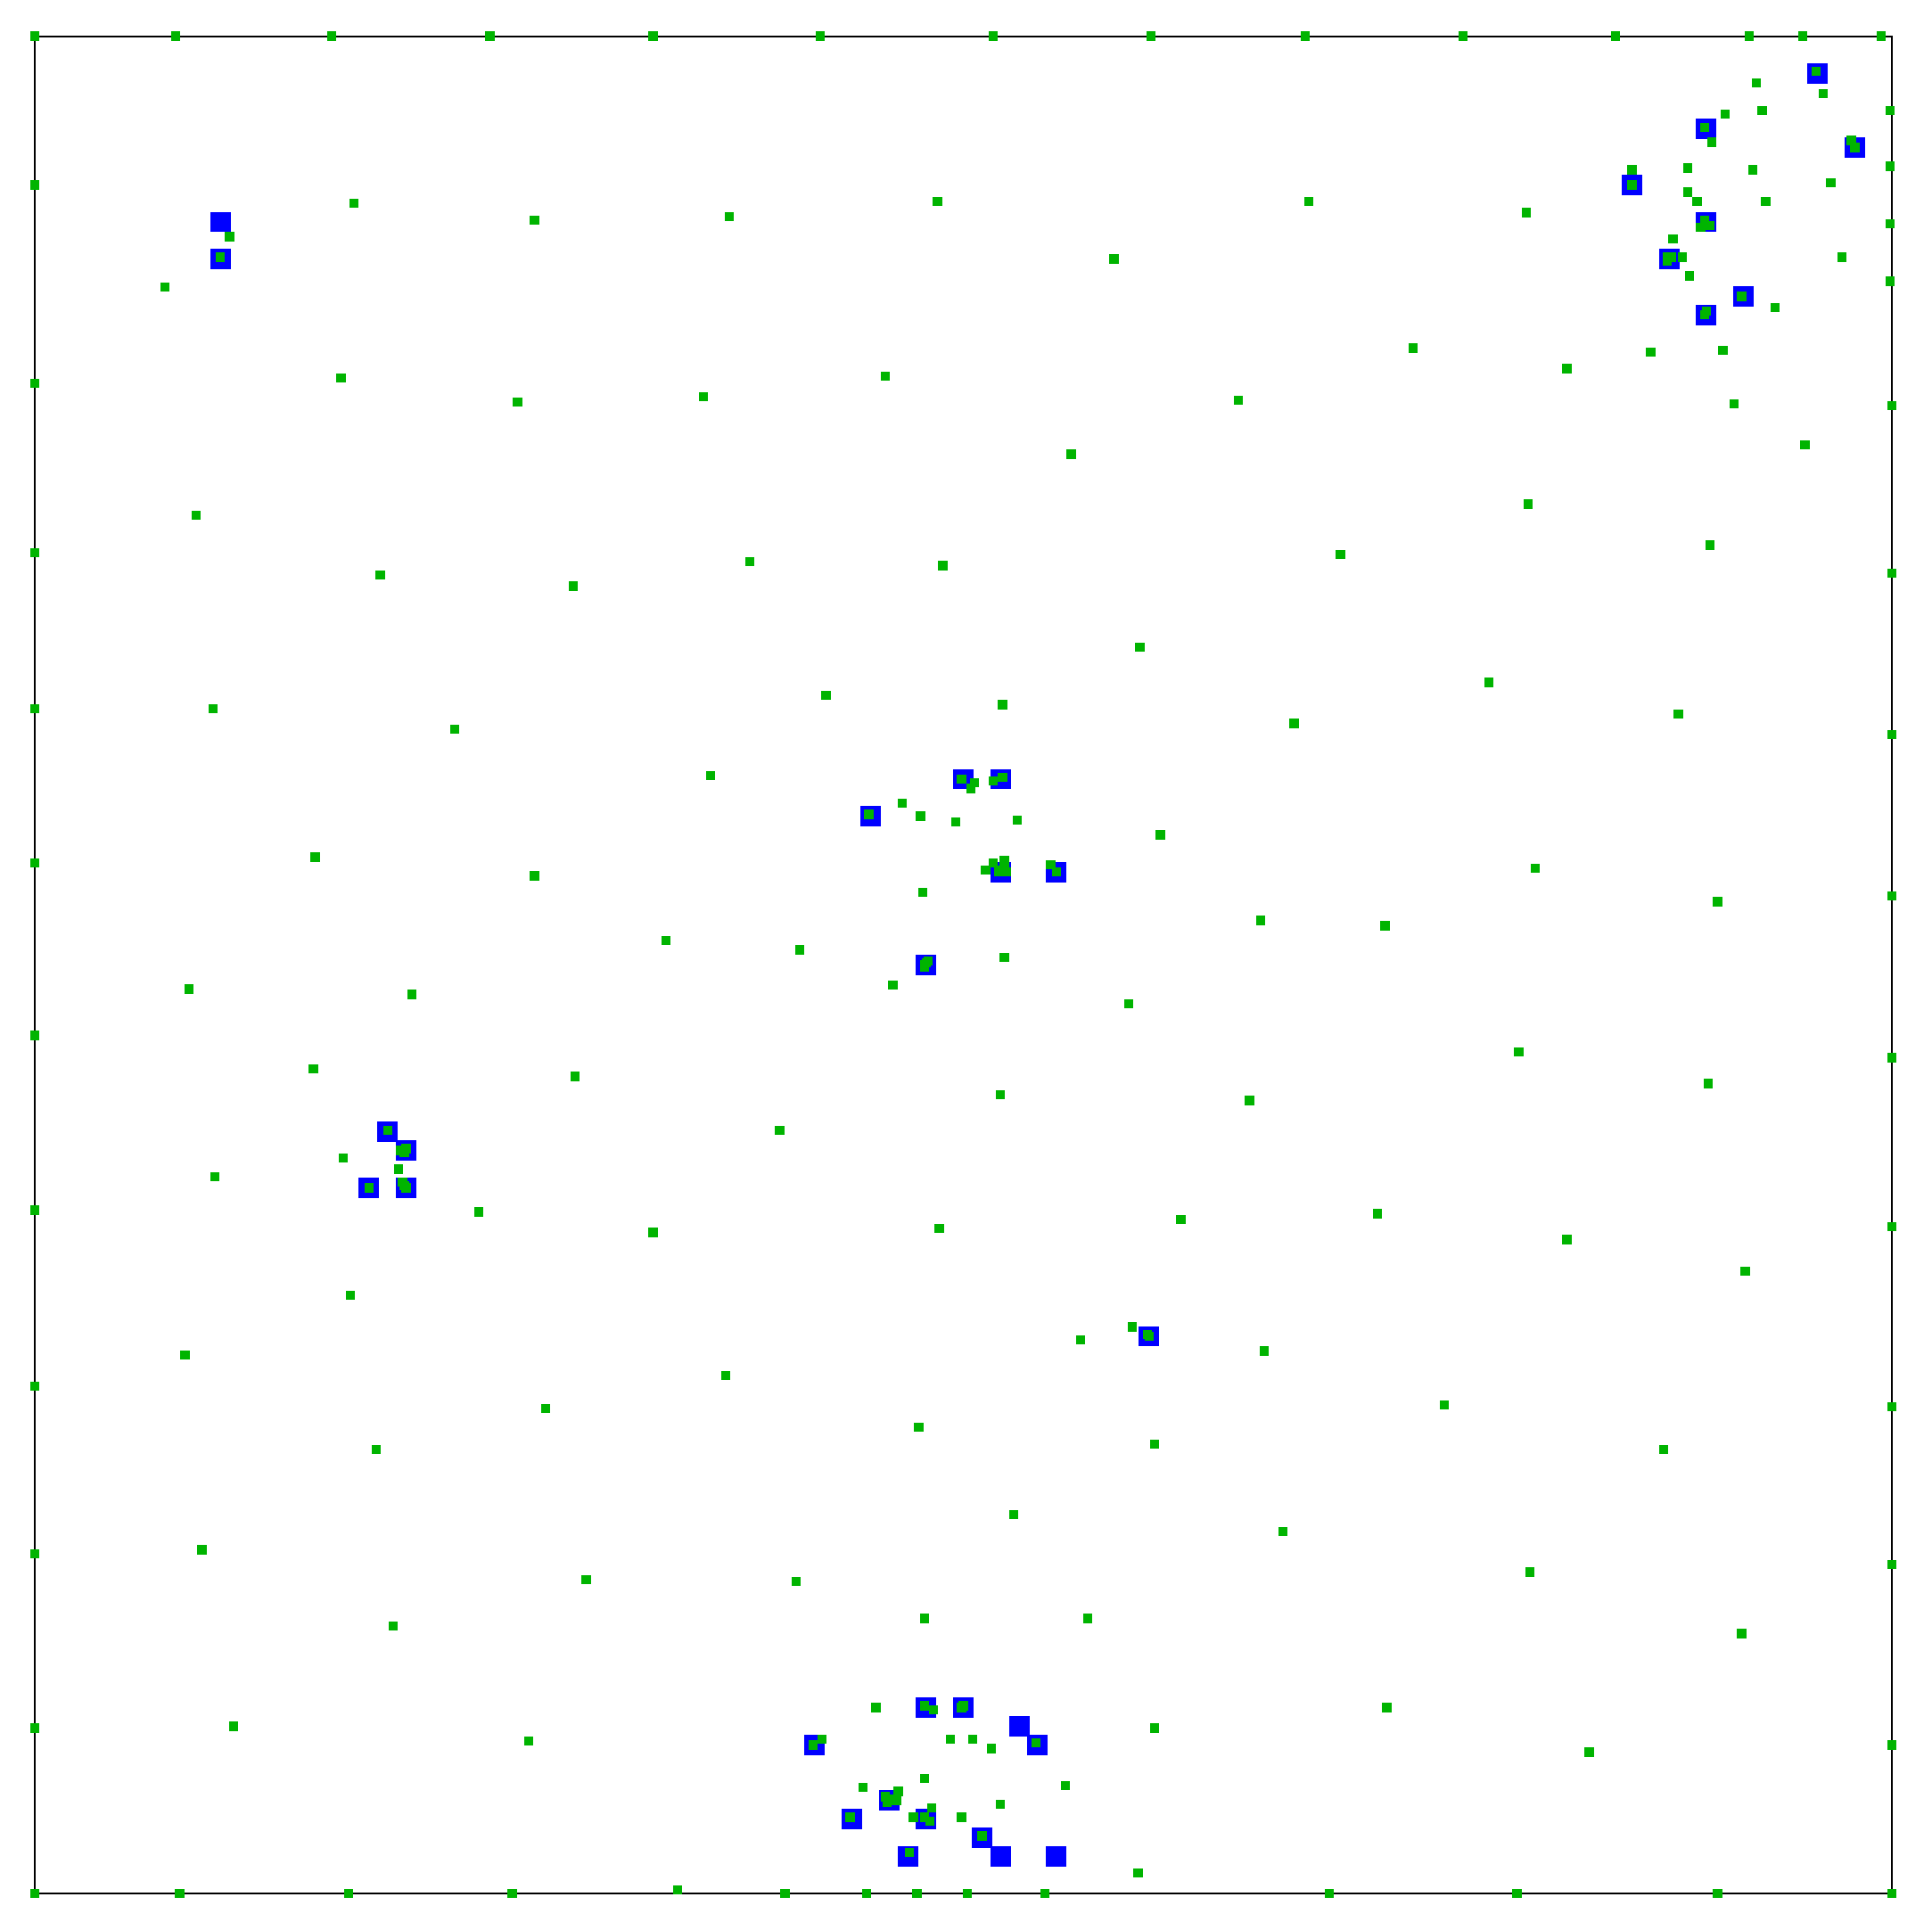
\includegraphics[width=0.5\textwidth]{img/usage/usage0.8-full.eps}}
  \caption{Test odpudivosti uzl�, vliv napln�nosti $=0,8$.}
  \label{fig:usage-ag-0.8}
\end{figure}

\begin{figure}[p]
  \centering
  \subfloat[EmptyRoom]{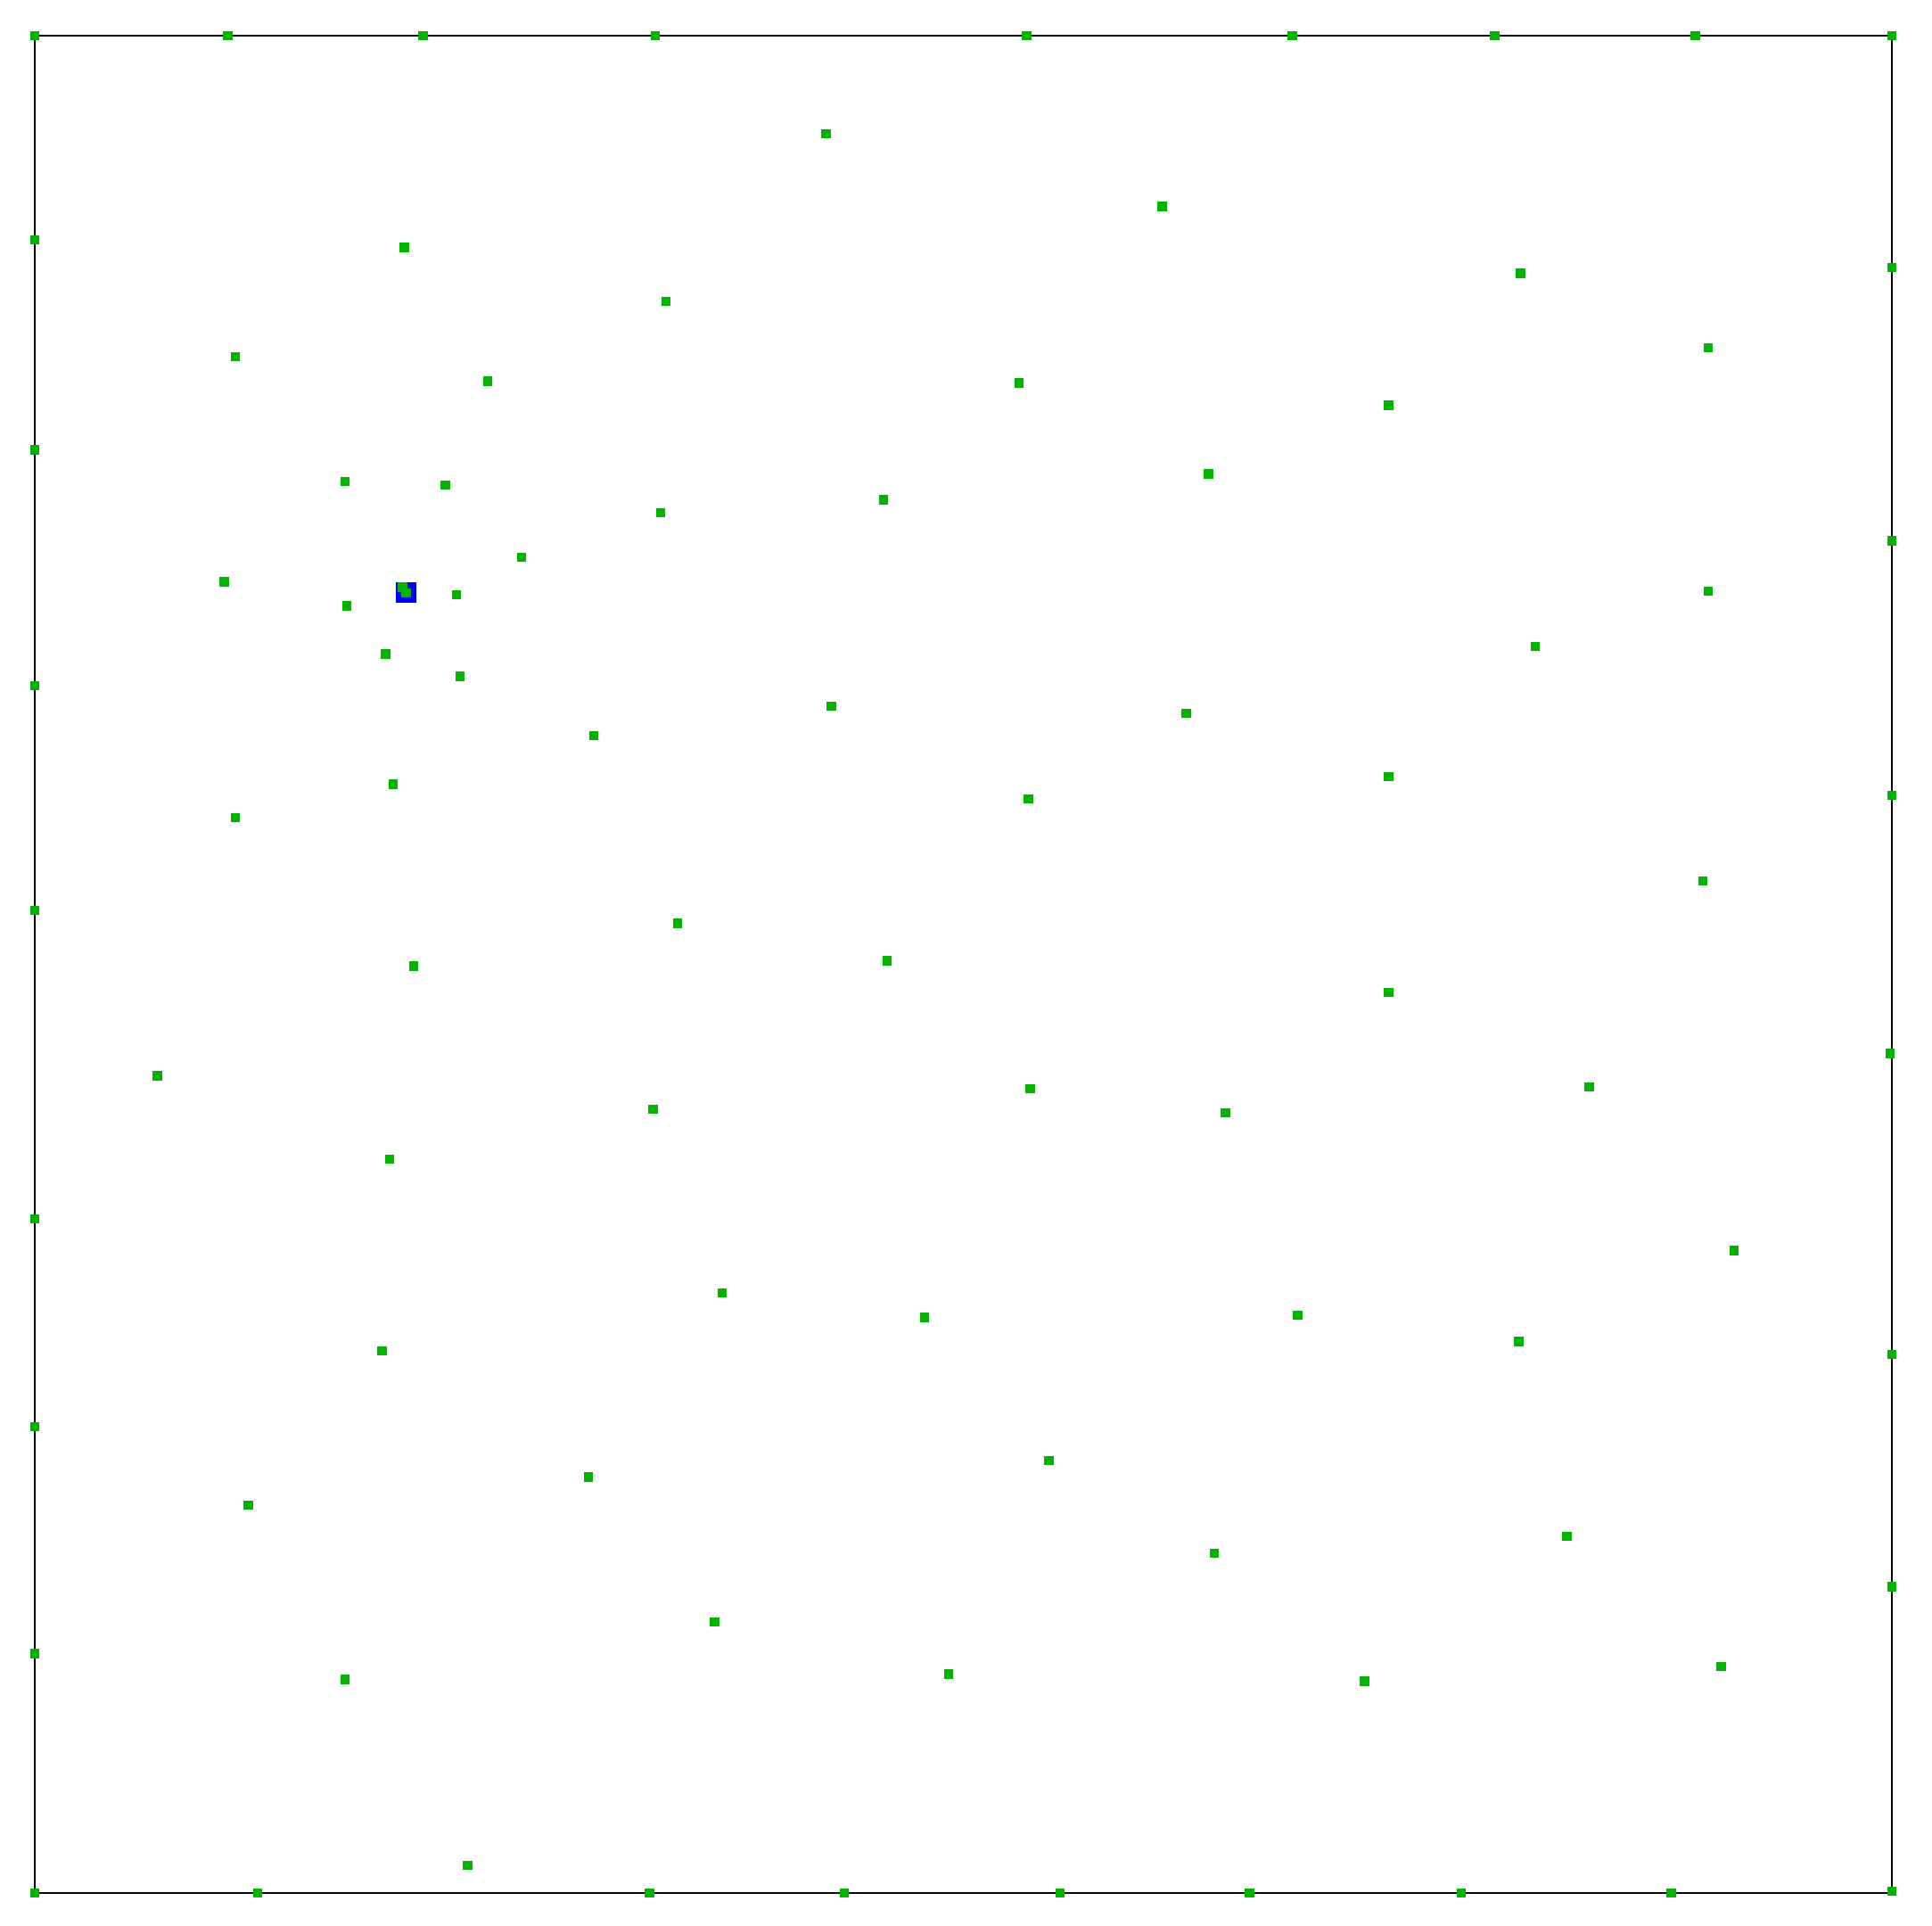
\includegraphics[width=0.5\textwidth]{img/usage/usage0.5-empty.eps}}
  \subfloat[FullRoom]{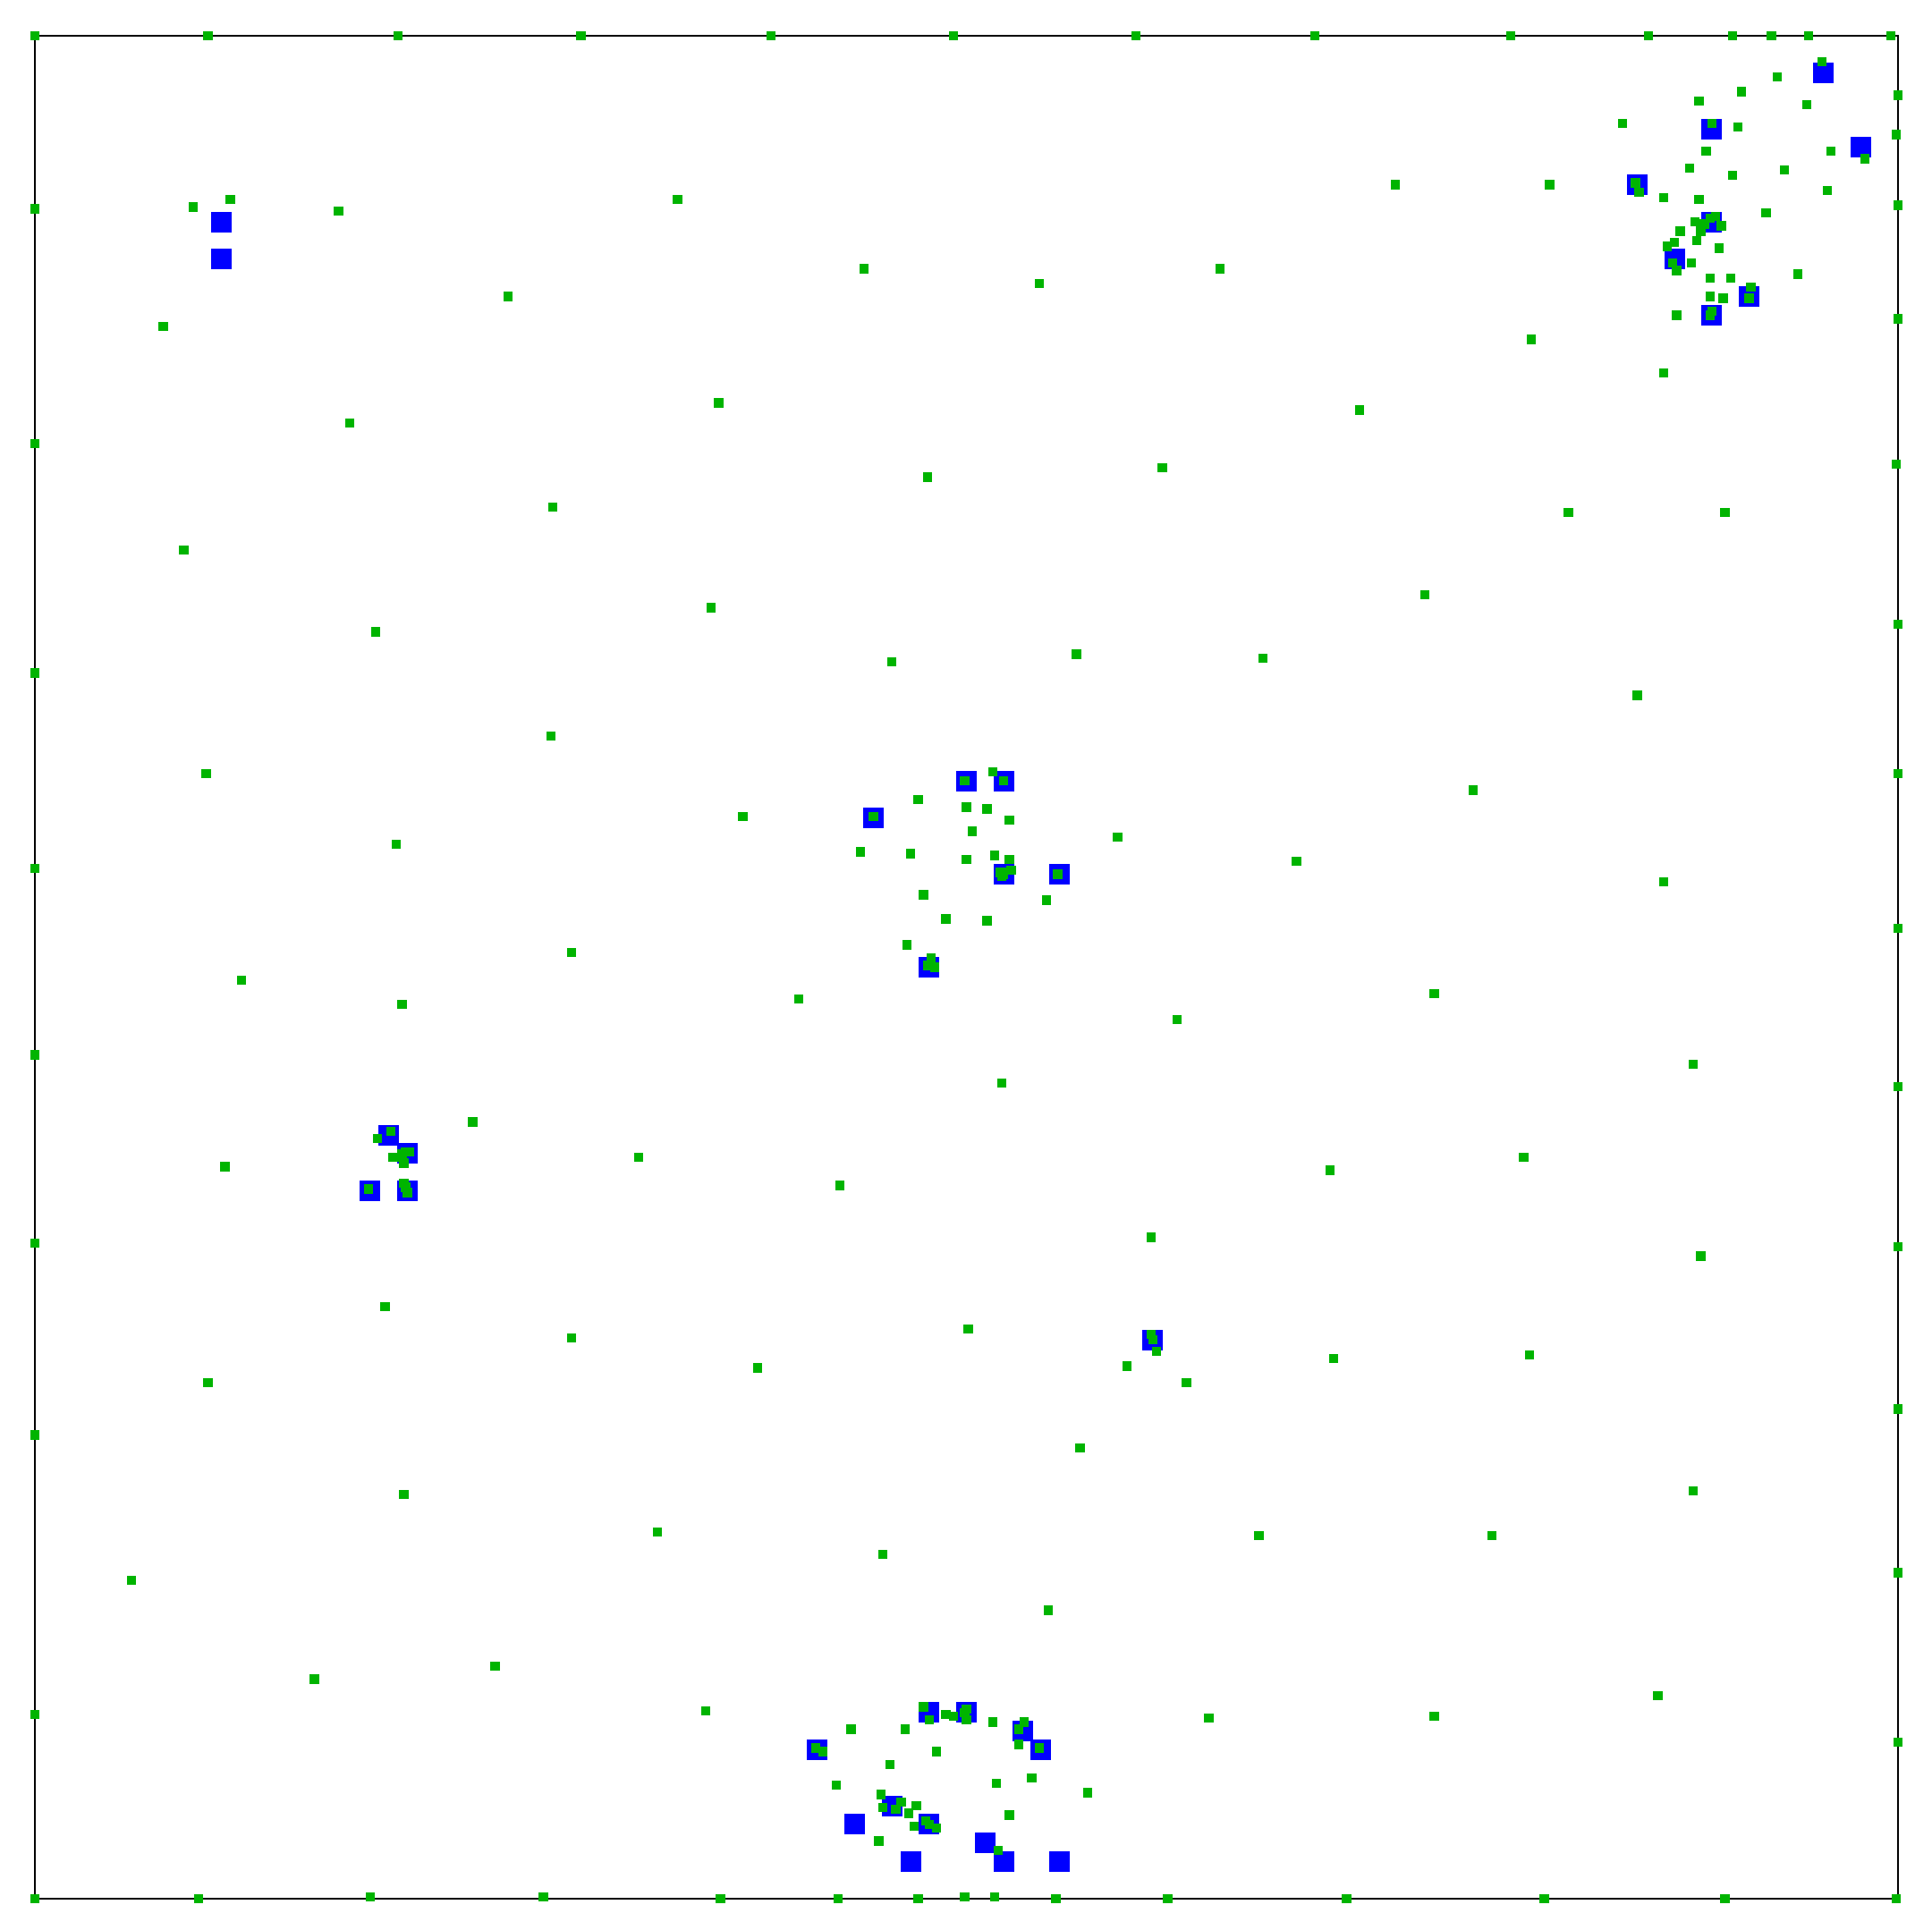
\includegraphics[width=0.5\textwidth]{img/usage/usage0.5-full.eps}}
  \caption{Test odpudivosti uzl�, vliv napln�nosti $=0,5$.}
  \label{fig:usage-ag-0.5}
\end{figure}



\newpage

\section{P�esnost mapy}
Jedn�m z objektivn�ch krit�ri� modelu je p�esnost mapy, nakolik odpov�d� realit� virtu�ln�ho sv�ta.

\begin{definition}[Nau�enost p�edm�tu]
V pr�b�hu simulace agent vid� a pou��v� p�edm�ty a prostorov� mapa dost�v� vjemy, kter� to odr�ej�.
Nau�enost p�edm�tu je vlastnost vyjad�uj�c� po�et a intenzitu vjem� dan�ho p�edm�tu.
Na za��tku simulace je rovna nule. V pr�b�hu simulace poka�d�, kdy� je vytvo�en vjem p�edm�tu, je nau�enost p�edm�tu zv��ena o intenzitu vjemu.
Nau�enost p�edm�tu nekles�.
\end{definition}

Na konci simulace m�me k dispozici mno�inu p�edm�t�, jejich polohu a nau�enost\footnote{Tyto informace jsou nez�visl� na prostorov� map�.}.
Prostorov� mapa m� k dispozici mno�inu uzl�, jejich polohu a napln�nost. P�edpokl�d�me, �e napln�nost uzl� bude odr�et nau�enost p�edm�t�.
Vizualizace dat pro m�stnost FullRoom je na obr�zku \ref{fig:test-heatmap}, dal�� jsou na p�ilo�en�m CD.
Ukazuje, �e n� p�epoklad je spr�vn�, uzly prostorov� mapy, resp. jejich napln�nost se bl�� nau�enosti p�edm�t�.
\\


\begin{figure}[h]
  \centering
  \subfloat[Nau�enost p�edm�t�]{\includegraphics[width=0.5\textwidth]{img/heatmap/predmet.eps}}
  \subfloat[Napln�nost uzl�]{\includegraphics[width=0.5\textwidth]{img/heatmap/uzel.eps}}
  \caption{Vizualizace napln�nosti uzl� a nau�enosti p�edm�t�.}
  \label{fig:test-heatmap}
\end{figure}

\newpage

Dal��m mo�n�m m���tkem je p�esnost zapamatovan�ch poloh p�edm�t�.
V ka�d�m kroku simulace m��eme ur�it polohu, o n� se agent domn�v�, �e na n� p�edm�t je.
Tuto domn�lou polohu m��eme porovnat s skute�nou polohou p�edm�tu.
Na obr�zc�ch \ref{fig:test-error1} a \ref{fig:test-error2} je zobrazen v�voj rozd�lu mezi realitou a agentovou prostorovou mapu v
�ase\footnote{V�sledky v dal��ch m�stnostech jsou op�t na p�ilo�en�m CD.}.
V tomto testu model usp�l jen v polovin� testovan�ch dat.
\\


\begin{figure}[h]
  \centering
  \subfloat[M�stnost Corridor]{\includegraphics[width=0.5\textwidth]{img/error/corridor.eps}}
  \subfloat[M�stnost CrazyRoom]{\includegraphics[width=0.5\textwidth]{img/error/crazy.eps}}
  \caption{Pr�m�rn� chyba polohy p�edm�t� v �ase.}
  \label{fig:test-error1}
\end{figure}

\begin{figure}[h]
  \centering
  \subfloat[M�stnost FullRoom]{\includegraphics[width=0.5\textwidth]{img/error/full.eps}}
  \subfloat[M�stnost HeapRoom]{\includegraphics[width=0.5\textwidth]{img/error/heap.eps}}
  \caption{Pr�m�rn� chyba polohy p�edm�t� v �ase.}
  \label{fig:test-error2}
\end{figure}

\newpage

\section{Test limit� m�st}
V kapitole \ref{chapter-place-detect} byl pops�n mechanismus vytv��en� m�st.
Model prostorov� mapy je tak schopen rozpoznat oblasti s vy��� hustotou uzl� a vytvo�it v takov� oblasti m�sto.
V tomto testu jsme se rozhodli vyzkou�et vliv parametr� \param{rychlost kles�n� $\varrho$}, \param{limit vzniku podm�sta} a \param{limit zapomenut� m�sta}.
Test jsme provedli s nastaven�m parametr� tak, aby do�lo k vytvo�en� v�ce m�st, jejich hodnoty jsou v tabulce \ref{tab:test-mist}, test m�l 4000 krok� simulace.
\\

\begin{table}[h!]
\begin{center}
\begin{tabular}{lcc}\toprule[0.5pt]

Parametr & V�choz� hodnota & Testovan� hodnota \\
\midrule[0.2pt]

ELAGFadeOut & 0,1 & 0,05 \\

PlacesAGNeeded & 1500 & 1000 \\

PlacesAGMin & 500 & 300 \\

\bottomrule[0.5pt]
\end{tabular}
\end{center}
\centering
\caption{Hodnoty parametr� testu}
\label{tab:test-mist}
\end{table}

V�sledky testu s v�choz�mi hodnotami parametr� jsou na obr�zku \ref{fig:test-places-ll}, v�sledky testu se zm�n�n�mi parametry jsou na obr�zku \ref{fig:test-places-lh}.
Je vid�t, �e zm�na testovan�ch parametr� zp�sobila vznik v�ce m�st. I v t�m�� pr�zdn� m�stnosti vznikla t�i m�sta.
\\

Vedlej��m efektem v�ak bylo vytvo�en� m�st i tam, kde jsme je neo�ek�vali a necht�li.
Zv�razn�n� m�sta na obr�zku \ref{fig:test-places-lh-heap} nevznikla p��mo d�ky hustot� uzl�.
Ke sv�mu vzniku spot�ebovala mno�stv� odpudivosti nahromad�n� v uzlech v t�sn� bl�zkosti jin�ch m�st.
\\


\begin{figure}[p]
  \centering
  \subfloat[EmptyRoom]{\includegraphics[width=0.5\textwidth]{img/places/lh-empty.eps}}
  \subfloat[HeapRoom]{\includegraphics[width=0.5\textwidth]{img/places/lh-heap.eps}}
  \caption{Test vytv��en� m�st, v�choz� hodnoty parametr�.}
  \label{fig:test-places-ll}
\end{figure}

\begin{figure}[p]
  \centering
  \subfloat[EmptyRoom]{\includegraphics[width=0.5\textwidth]{img/places/ll-empty.eps}}
  \subfloat[HeapRoom]{\label{fig:test-places-lh-heap}\includegraphics[width=0.5\textwidth]{img/places/ll-heap.eps}}
  \caption{Test vytv��en� m�st, zm�n�n� hodnoty parametr�.}
  \label{fig:test-places-lh}
\end{figure}




\newpage

\section{Test dynamick�ho sv�ta}
Model prostorov� mapy je vytvo�en tak, aby se dok�zal p�izp�sobit m�n�c�mu se prost�ed�.
Provedli jsme test v m�stnosti SwitchRoom, kterou jsme navrhli pr�v� pro tento ��el.
V m�stnosti dojde ke dv�ma zm�n�m, v kroku 1500 je odebr�na ��st p�edm�t� a v kroku 4000 je n�kolik z nich vr�ceno zp�t a vytvo�eno n�kolik
nov�ch\footnote{M�stnost SwitchRoom a jej� zm�ny jsou zobrazeny v p��loze A}.
\\

V�sledek testu je na obr�zc�ch \ref{fig:test-dyn-nc} a \ref{fig:test-dyn}. Je na nich vid�t, �e mapa se skute�n� p�izp�sobila nov�m p�edm�t�m
p�idan�m v kroku 4000 v doln�m prav�m rohu a brzy tam vzniklo m�sto.
Po�et uzl� mapy tak� zareagoval na zm�nu po�tu p�edm�t�, kr�tce po kroku 1500 p�estal r�st, pozd�ji za�al zvolna klesat.
Kdy� byly p�id�ny nov� p�edm�ty, po�et uzl� za�al pozvolna stoupat.
Pr�b�h testu je l�pe vid�t na videu, kter� je na p�ilo�en�m CD.
\\

\begin{figure}[h!]
  \centering
  \includegraphics[width=0.9\textwidth]{img/dyn/nc.eps}
  \caption{Po�et uzl� prostorov� mapy v �ase, testovac� m�stnost SwitchRoom.}
  \label{fig:test-dyn-nc}
\end{figure}

\begin{figure}[!h]
  \centering
  \subfloat[Krok 4001]{\includegraphics[width=0.5\textwidth]{img/dyn/step4001.eps}}
  \subfloat[Krok 4400]{\includegraphics[width=0.5\textwidth]{img/dyn/step4400.eps}}
  \caption{Test dynamick�ho sv�ta, v kroku 4000 jsou p�id�ny p�edm�ty do prav�ho doln�ho rohu, v kroku 4400 tam ji� je m�sto.}
  \label{fig:test-dyn}
\end{figure}
\chapter{Diskuze}

Mo�n� roz���en�
� Zm�na Agcoef a AGrange v �ase, glob�ln� �i l�pe pro ka�d� uzel, dle Agamount (nem�-li se s k�m odpuzovat v okol�, zv�t�� si okol� a s�lu
\\

� Sjednocen� EP, ELnode - ka�d� m� �ivotnost - bu� v�ce �rovn�, �i spojit� m�ra �rovn� - ka�d� uzel m� jak moc miz� apod.
\\

� Snadn� roz���en� do 3D
\\

� Hiearchie/ontologie affordanc�, pro shlukov�n� p�edm�t� dle toho �i dle topologie
\\

� Druh�m p�ijemn�m v�sledkem je, �e model lze snadno roz���it pro sv�ty v�t�� ne� jeden uzav�en� prostor, pokud agent bude zn�t topologii sv�ta. Toto roz���en� je podrobn�ji pops�no v sedm� kapitole.
\\

� Ukl�dat do uzlu i co agent d�lal - tj. EP kter� m�sto MO bude m�t Process
	0 Dal��  mapa ukl�daj�c� pouze to
	0 I co vid�l, �e d�laj� dal�� agenti
\\

� Model lze pou��t i na odli�n� v�ci jako
	0 Hran� pexesa
	0 Nau�en� se rozlo�en� kl�ves na kl�vesnici
\\
\chapter{Z�v�r}

�eho bylo dosa�eno, co model um�, co ne

shrnuti mo�n�ch roz���en� z diskuze

Poda�ilo se vytvo�it model spl�uj�c� po�adavky, tedy 
U��c� se online
Rozprost�r� uzly do prostoru stejn� jako jsou objekty
Umo��uje ukl�dat informaci o poloze objekt�


\appendix


\chapter{Testovac� m�stnosti}

Pro ��ely testov�n� modelu jsme vytvo�ili 9 testovac�ch sv�t�:
\\

\begin{CompactItemize}
\item FullRoom - �tvercov� m�stnost s 33 p�edm�ty
\item EmptyRoom - �tvercov� m�stnost s jedn�m p�edm�tem
\item Corridor - chodba s 10 p�edm�ty
\item Lobby - slo�it�j�� m�stnost s 30 p�edm�ty
\item CrazyRoom - velmi slo�it� m�stnost s 24 p�edm�ty
\item SmallRoom - men�� m�stnost s 14 p�edm�ty
\item SwitchRoom - m�stnost je na za��tku stejn� jako FullRoom, v pr�b�hu se m�n�
\item HeapRoom - m�stnost pro testov�n� hierarchie modelu a detekce m�st
\item HeapLineRoom - m�stnost pro testov�n� hierarchie modelu a detekce m�st
\end{CompactItemize}

Sv�ty resp. m�stnosti jsou zobrazeny na n�sleduj�c�ch str�nk�ch. Modr� �tverce jsou p�edm�ty, men�� �ern� jsou waypointy.
\\

\begin{figure}
  \centering
  \subfloat[FullRoom]{\label{fig:fullroom}\includegraphics[width=0.5\textwidth]{img/rooms/fullroom.eps}}
  \subfloat[EmptyRoom]{\label{fig:emptyroom}\includegraphics[width=0.5\textwidth]{img/rooms/emptyroom.eps}}
  \caption{Jednoduch� m�stnosti}
  \label{fig:simlpe-rooms}
\end{figure}

\begin{figure}
  \centering
  \subfloat[Corridor]{\label{fig:corridor}\includegraphics[width=0.5\textwidth]{img/rooms/corridor.eps}}
  \subfloat[Lobby]{\label{fig:lobby}\includegraphics[width=0.5\textwidth]{img/rooms/lobby.eps}}
  \caption{Slo�it�j�� m�stnosti}
  \label{fig:advanced-rooms}
\end{figure}

\begin{figure}
  \centering
  \subfloat[CrazyRoom]{\label{fig:crazyroom}\includegraphics[width=0.5\textwidth]{img/rooms/crazyroom.eps}}
  \subfloat[SmallRoom]{\label{fig:smallroom}\includegraphics[width=0.5\textwidth]{img/rooms/smallroom.eps}}
  \caption{Slo�it�j�� m�stnosti}
  \label{fig:advanced-rooms2}
\end{figure}

\begin{figure}
  \centering
  \subfloat[HeapRoom]{\label{fig:heaproom}\includegraphics[width=0.5\textwidth]{img/rooms/heaproom.eps}}
  \subfloat[HeapLineRoom]{\label{fig:heaplineroom}\includegraphics[width=0.5\textwidth]{img/rooms/heaplineroom.eps}}
  \caption{M�stnosti pro testov�n� hierarchie modelu a vytv��en� m�st}
  \label{fig:heaprooms}
\end{figure}

\begin{figure}
  \centering
  \subfloat[Krok 0]{\label{fig:switchroom-1}\includegraphics[width=0.4\textwidth]{img/rooms/switchroom-1.eps}}
  \quad
  \subfloat[Krok 1500]{\label{fig:switchroom-2}\includegraphics[width=0.4\textwidth]{img/rooms/switchroom-2.eps}}
  \quad
  \subfloat[Krok 4000]{\label{fig:switchroom-3}\includegraphics[width=0.4\textwidth]{img/rooms/switchroom-3.eps}}
  \caption{M�stnost SwitchRoom a jej� prom�ny v �ase}
  \label{fig:switchroom}
\end{figure}


\chapter{Parametry modelu}


\begin{table}[h!]
\begin{center}
\begin{tabular}{|l|l|r|r|}\hline

\param{Maxim�ln� krok agenta} & \texttt{MaxAgentMove} & 10 & 2 - 20 \\
\hline

\param{Velikost waypointu} & \texttt{WayPointArea} & 10 & 5 - 20 \\
\hline

\param{Odchylka waypointu} & \texttt{WayPointNoise} & 10 & 0 - 20 \\
\hline

\param{Velikost percep�n�ho pole} & \texttt{PFSize} & 7 & 5 - 9 \\
\hline

\param{Vzd�lenost nutn� k pou�it� p�edm�tu} & \texttt{MapPickUpDistance} & 2 & 1 - 5 \\
\hline

\param{V�choz� atraktivita p�edm�t�} & \texttt{ObjDefaultAttractivity} & 1 & 0,5 - 2 \\
\hline

\end{tabular}
\end{center}
\centering
\caption{Parametry sv�ta a agenta}
\label{tab:typy-vjemu}
\end{table}




\begin{table}[h!]
\begin{center}
\begin{tabular}{|p{6cm}|l|l|l|}\hline


\param{Efekt zpozorov�n� p�edm�tu} & \texttt{TrainEffectNoticed} & 1 & 1 \\
\hline

\param{Efekt zpozorov�n� p�edm�tu znovu} & \texttt{TrainEffectNoticedAgain} & 0,3 & 0,1 - 0,5 \\
\hline

\param{Efekt pou�it� p�edm�tu} & \texttt{TrainEffectUsed} & 3 & 1 - 10 \\
\hline

\param{Efekt nalezen� p�edm�tu} & \texttt{TrainEffectFound} & 2 & 1 - 3 \\
\hline

\param{Efekt nenalezen� p�edm�tu} & \texttt{TrainEffectNotFound} & -1 & -1 \\
\hline

\param{Maxim�ln� d�lka atomick� akce, pokud je del��, provede prostorov� pam� v�ce krok�} & \texttt{SMUpdateMaxDuration} & 100 & 10 - 10000 \\
\hline

\param{Dosah u�en�} & \texttt{SMTrainRange} &  10 & 10 - 20 \\
\hline

\param{Po��te�n� napln�nost uzlu} & \texttt{MemObjIntenseToNewNode} & 1 & 1 - 5 \\
\hline

\param{M�ra zapom�n�n� pam�ov�ch stop p�edm�t�} & \texttt{MemObjIntensityFadeOut} &   0,01 & 0,001 - 0,1 \\
\hline

\param{M�ra zapom�n�n� vazeb mezi uzly a pam�ov�mi stopami} & \texttt{LinkMemObjToNodeFadeOut} & 0,005 & 0,001 - 0,1 \\
\hline

\end{tabular}
\end{center}
\centering
\caption{Parametry pam�ti na p�edm�ty}
\label{tab:typy-vjemu}
\end{table}






\begin{table}[h!]
\begin{center}
\begin{tabular}{|l|l|r|r|}\hline

\param{Hustota mapy} & \texttt{ELDensity} & 10 & 10 \\
\hline

\param{Po��te�n� odchylka mapy} & \texttt{ELCreateNoise} & 3 & 1 - 5 \\
\hline

\param{Rychlost kles�n� napln�nosti} & \texttt{ELNodeUsageFadeOut} & 0,005 & 0,001 - 0,01 \\
\hline

\param{Dosah p�ita�livosti} & \texttt{ELGravityRange} & 20 & 10 - 30 \\
\hline

\param{S�la p�ita�livosti} & \texttt{ELGravityCoef} & 1 & 0,2 - 3 \\
\hline

\param{Dosah odpudivosti} & \texttt{ELAntigravityRange} & 20 & 10 - 30 \\
\hline

\param{S�la odpudivosti} & \texttt{ELAntigravityCoef} &  8 & 4 - 20 \\
\hline

\param{Vliv napln�nosti} & \texttt{ELAGUsageCoef} & 0,8 & 0,4 - 1 \\
\hline

\param{Limit pohybu uzlu} & \texttt{MaxELNodeMove} &  4 & 1 - 5 \\
\hline

\param{Vliv vjemu} & \texttt{EPCreateEnergy} &  140 &  100 - 200\\
\hline

\param{Odchylka vytvo�en� uzlu} & \texttt{ELNodeAddNoise} &  2  & 1 - 5 \\
\hline

\param{M�ra slabnut� stopy vjemu} & \texttt{EPFadeCoef} & 0,5  & 0 - 0,9 \\
\hline

\param{Limit zmizen� stopy vjemu} & \texttt{EPFadeLimit} &  10 & 1 - 20 \\
\hline

\param{M�ra zapom�n�n� uzl�} & \texttt{ELForgetNodeRate} & 5 & 1 - 10 \\
\hline

\param{Po�et opakov�n�} & \texttt{ELDeleteNodeReTrainCount} & 20 & 10 - 50 \\
\hline

\param{Velikost okol�} & \texttt{ELDeleteNodeReTrainRange} & 20 & 5 - 40 \\
\hline

\param{Rychlost r�stu $\varrho$} & \texttt{ELAGAddCoef} &  3 & 1 - 5 \\
\hline

\param{Rychlost kles�n� $\varrho$} & \texttt{ELAGFadeOut} &  0,1 & 0,01 - 1 \\
\hline

\param{Limit vzniku podm�sta} & \texttt{PlacesAGNeeded} &  1500 & 500 - 5000 \\
\hline

\param{Limit zapomenut� m�sta} & \texttt{PlacesAGMin} &  500 & 100 - 200 \\
\hline

\param{Rychlost r�stu intenzity} & \texttt{PlacesAGGrow} &  0,1 & 0,01 - 0,5 \\
\hline

\param{Rychlost kles�n� intenzity} & \texttt{PlaceAGFadeOut} &  0,5 & 0,1 - 1 \\
\hline

\param{Pohyblivost m�st} & \texttt{PlaceMoveCoef} &  0,02 & 0,01 - 0,5 \\
\hline

\end{tabular}
\end{center}
\centering
\caption{Parametry gravita�n�ho modelu vrstvy uzl�}
\label{tab:typy-vjemu}
\end{table}

\chapter{U�ivatelsk� dokumentace}

\section{Instalace}
Nejd��ve je t�eba nainstalovat pot�ebn� knihovny:

- Python
 - GTK+

Pro vizualizaci v�stupn�ch dat je t�eba nainstalovat
- knihovnu numpy
- knihovnu matplotlib
- .Net Framework 3.5


\section{Ovl�d�n� aplikace}
Aplikace se spou�t� hlavn�m souborem mainGUI.py.


\section{V�stupn� data a jejich vizualizace}

V�stupem aplikace jsou:
\begin{CompactItemize}
\item obr�zky ukazuj�c� stav sv�ta a prostorov� mapy v ka�d�m kroku simulace
\item obr�zek ukazuj�c� stav v posledn�m kroku simulace v�etn� nau�enosti p�edm�tu (jak moc se jej agent m�l �anci nau�it, nez�visle na prostorov� map�)
\item textov� soubory ve form�tu CVS
\end{CompactItemize}

Data v textov�ch souborech je mo�n� vizualizovat pou�it�m n�stroj� statter.exe\footnote{
statter.exe je pot�eba pouze, pokud u�ivatel chce vid�t podrobn� informace o stavu uzl� prostorov� mapy v pr�b�hu simulace} a plotter.py.

\chapter{Program�torsk� dokumentace}

Model popsan� v kapitole ?? jsme 

zakladni myslenky implementace

pouzite veci
python
tkinter
PIL

numpy
matplotlib
statter a plotter

pojmenovani trid a mapovani modelu do implementace


Ve sv�t� m��e zat�m b�t pr�v� jeden agent.

efektivita - pomale protoze aritmetika v pythonu

??? reference vygenerovana z kmentaru ???
\chapter{Obsah p�ilo�en�ho DVD}

Sou��st� pr�ce je tak� p�ilo�en� DVD, kter� obsahuje prototypovou aplikace a v�sledky v�ech uveden�ch test�.
Sou��st� testu je v�dy zdrojov� k�d, kter� byl testov�n, v�stupn� data v�etn� vizualizace a t�m�� v�dy video zachycuj�c� pr�b�h testu.
\\

\begin{description}
  \setlength{\leftmargin}{0.5cm}
  \setlength{\itemsep}{5pt}
  \setlength{\parsep}{0pt}
  \setlength{\topsep}{0pt}
\item[\texttt{app/app}]  \hfill \\
  prototypov� aplikace a pomocn� n�stroje v�etn� zdrojov�ch k�d�
\item[\texttt{app/doc}]  \hfill \\
  podrobn� program�torsk� dokumentace vygenerovan� z koment���
\item[\texttt{app/install}]  \hfill \\
  knihovny pot�ebn� pro b�h aplikace
\item[\texttt{obrazky/}]  \hfill \\
  obr�zky m�stnosti a uk�zky po��te�n�ho rozlo�en� uzl�
\item[\texttt{testy/\_kohonen}]  \hfill \\
  testy modelu zalo�en�ho na Kohonenov� map�
\item[\texttt{testy/\_final}]  \hfill \\
  testy v�sledn�ho modelu
\item[\texttt{testy/*}]  \hfill \\
  dal�� testy
\end{description}




\bibliographystyle{jk}
\bibliography{literatura}

\end{document}
